% Generated body; only mechanical merging changes.



\begin{abstract}\noindent
We compute the scaling dimension $\De$ of the energy operator of the one-dimensional long-range Ising model, with couplings
decaying as $1/r^{1+s}$, at thirteen values of the spin dimension $\Ds=(1-s)/2$ between $0.249$ and $0.001$. The critical point is
realized as the quantum critical point of the sub-ohmic spin--boson model, which we solve with a bosonic numerical renormalization
group (NRG); the relevant eigenvalue $y_t=1-\De$ is obtained from the exact derivative of the truncated NRG map with respect to the
bath coupling. At ten points, $0.001\le\Ds\le0.2$, we give final values, for example $\De=\nrgDEOneHundred$ at $s=0.8$ and
$\nrgDETwoHundred$ at $s=0.6$. At eight of them, $0.001\le\Ds\le0.15$, the local exponent settles on a plateau along the chain, and
the error scales are $\nrgerrLow$ for $0.01\le\Ds\le0.125$, $\nrgerrOneFifty$ at $\Ds=0.15$ and $\nrgerrOne$ at $\Ds=0.001$. At
$\Ds=0.175$ and $0.2$ the local exponent is still drifting at the end of the usable chain and is extrapolated, with error scales
$\nrgerrOneSeventyFive$ and $\nrgerrTwoHundred$. Each error adds three parts linearly: the drift along the chain, the spread over kept
states and oscillator levels, and a discretization error, the larger of the spread over the values of $\Lambda$ that were run and the
change of the $\Lambda=2.5$ value when the number of kept states is doubled; the latter sets it at $\nrgnLambdaKdbl$ of the 10 final
points. The errors are not standard deviations. Near $s=1/2$ the leading correction exponent $\omega\approx\varepsilon$ vanishes, and
within the chain depth reachable in double precision the flow does not reach its fixed point: at $\Ds=0.249$, $0.24$ and $0.225$ the
values where it comes closest lie $\nrgexcTwoFortyNine$, $\nrgexcTwoForty$ and $\nrgexcTwoTwentyFive$ above the $\varepsilon$
expansion, and at $\Ds=0.249$ the inverse excess grows along the renormalization-group time at a rate of the size that one loop
predicts. We label these three points not converged in chain depth, a label assigned after the comparison with the series, show
their values, and use them in no comparison. Near $s=1$ the results reproduce the strong--weak dual expansion of $\De$ through its
fifth coefficient. At the $\nrgmcAccN$ points where the project's cluster Monte Carlo study accepts its own value, NRG differs from it
by at most $\nrgmcAccDiffMax$. That is within the sum of the Monte Carlo statistical error, its fit-model half-range and the NRG
error at $\nrgmcAccWithinLin$ points, and $\nrgmcAccRatioMax$ times that sum at the fifth; but it is up to $\nrgmcAccStatRatioMax$
Monte Carlo statistical errors, with the same sign at neighboring points, so only the fit-model half-range reconciles the two. The
Monte Carlo crossing extrapolations agree with NRG within $\nrgmcCrossStatMax$ of their statistical errors at these points. A second
solver, written by a separate Claude agent from a physics-only specification, reproduces the chain coefficients to better than
$\nrgindChain$ (rounding level), the critical couplings bitwise or to $\nrgindAlpha$, and $\DE$ to $\nrgindDE$ in every window its
finite differences can reach. The code was written by GPT-6 astra (OpenAI) and ported to the cluster, run and analyzed by Claude Code
(Anthropic); every number in this note is regenerated from the released records by \code{make replay}.
\end{abstract}


\clearpage

% =====================================================================================================================
\section{Overview}\label{nrg:sec:overview}
% =====================================================================================================================
\subsection{Scope}
This note is written for a physicist outside the project. Section~\ref{nrg:sec:model} states the problem and what is known analytically.
Sections~\ref{nrg:sec:method} and~\ref{nrg:sec:budget} describe the numerical method, the estimator and the error budget in enough detail to
re-implement them. Section~\ref{nrg:sec:software} describes the code and how it was validated, Sec.~\ref{nrg:sec:campaigns} the production
runs, Sec.~\ref{nrg:sec:results} the results, and Sec.~\ref{nrg:sec:checks} the checks against a second implementation, against two methods
that do not use NRG and against published values. Section~\ref{nrg:sec:limits} collects the limitations and Sec.~\ref{nrg:sec:repro}
explains how to recompute every number. The appendices give the data formats (App.~\ref{nrg:app:formats}), the production on the
cluster (App.~\ref{nrg:app:cluster}), the provenance of code, analysis and review (App.~\ref{nrg:app:provenance}), every production run
(App.~\ref{nrg:app:items}), the estimator used before this revision and its values (App.~\ref{nrg:app:midpoint}), and the terms and symbols
(App.~\ref{nrg:app:symbols}).

\paragraph{Who did what.} The NRG solver was written by GPT-6 astra (OpenAI, through ChatGPT) in two stages: a reference solver for
an earlier, unreleased study of the project (the \emph{original study}; shipped as \code{code/lri\_spin\_boson\_hpc/reference/}) and
an optimized package built on it. Claude Code (Anthropic) reviewed the package, ported it to a Slurm cluster, ran the production,
wrote the analysis and drafted this note; OpenAI Codex reviewed the cluster port. Two rounds of read-only reviews of the analysis
and of this note, three reviews each, were made by Claude agents on 13 October 2026, and an independent reader reviewed the text on
15 October. This version follows them; the changes made after the second round and after the reading were not reviewed again.
There was no human referee. App.~\ref{nrg:app:provenance} gives the details, including which model ran where. In this note ``the
author'' is Z.~Zheng, who made the decisions marked as his, and ``we'' is the study as a whole: the author and the AI systems that
worked for him.

\paragraph{Vocabulary.} A \emph{point} is one value of $\Ds$. An \emph{item} is one complete NRG calculation at fixed
$(\Ds,\Lambda,K,n_b,N)$: the search for the critical coupling, the exact derivative of the critical flow, and the window audit
(Sec.~\ref{nrg:sec:method}). Its \emph{record} is the JSON file that holds the result. The \emph{central item} of a point is the one at
$\Lambda=3$, $K=128$, $n_b=16$; all other items are convergence scans. A \emph{campaign} is a set of items submitted together
(Sec.~\ref{nrg:sec:campaigns}), and \emph{production} means the $\nrgnItems$ items whose records are released. A \emph{window} is a
stretch of consecutive chain sites over which the growth of the derivative is fitted (Sec.~\ref{nrg:sec:windows}). We write $\DE$ for the
NRG estimate of $\De$; despite the notation it is not an energy difference. App.~\ref{nrg:app:symbols} lists all terms and symbols.

\subsection{Headline results}
Table~\ref{nrg:tab:headline} is the main result, and Fig.~\ref{nrg:fig:checks} shows it with the references of Sec.~\ref{nrg:sec:checks}.
``Final'' values are the estimates of Sec.~\ref{nrg:sec:estimator} with the total error $\dtot$ of Sec.~\ref{nrg:sec:budget}. The three values
in gray brackets are not converged in chain depth (Sec.~\ref{nrg:sec:approach}): they are shown, carry no error, and enter no comparison
and no agreement statement in this note. That label is not an outcome of the estimator; it was assigned after the comparison with
the $\varepsilon$ series (Sec.~\ref{nrg:sec:estimator}).

\begin{table}[ht]\centering\small\setlength{\tabcolsep}{4pt}
\caption{Thermal dimension $\De$ of the $d=1$ long-range Ising model from bosonic NRG: $\DE=1-y_t$ at $\Lambda=3$, $K=128$ kept states
per parity sector and $n_b=16$ oscillator levels, with the total error $\dtot$ in parentheses (Sec.~\ref{nrg:sec:budget}: chain depth
plus $K$/$n_b$ spread plus discretization error, the last mostly an allowance for the convergence in $K$ at $\Lambda=2.5$; PDG
rounding). ``Final'' is the plateau value of Sec.~\ref{nrg:sec:estimator}; ``final, extrapolated'' is the extrapolation of the local
exponent. Gray: not converged in chain depth; the settled value, no error, not used in any comparison, and its excess over the
$\varepsilon$ series in the last column. External test: the $\varepsilon$ series (Sec.~\ref{nrg:sec:series}), whose spread at $\Ds=0.2$
is far larger than the NRG error; the label that the Monte Carlo study gives its own value (Sec.~\ref{nrg:sec:mc}) and, where that value
is accepted, NRG minus Monte Carlo with its ratio to $\sigma_{\rm stat}+\sigma_{\rm sys}+\dtot$; at $\Ds\le0.01$ only the expansion
about $s=1$ of Sec.~\ref{nrg:sec:s1}.}\label{nrg:tab:headline}
\begin{tabular}{@{}lllll>{\raggedright\arraybackslash}p{6.4cm}@{}}
\toprule
$\Delta_\sigma$ & $s$ & $\varepsilon$ & $\Delta_E$ & status & external test (Sec.~\ref{nrg:sec:checks})\\
\midrule
0.249 & 0.502 & 0.004 & \textcolor{gray}{[0.5080]} & not converged & series 0.499344 (excess $+8.7\times10^{-3}$)\\
0.24 & 0.52 & 0.04 & \textcolor{gray}{[0.4989]} & not converged & series 0.49422 (excess $+4.7\times10^{-3}$)\\
0.225 & 0.55 & 0.1 & \textcolor{gray}{[0.4897]} & not converged & series 0.48808 (excess $+1.6\times10^{-3}$); MC label: conditional\\
0.2 & 0.6 & 0.2 & 0.4830(7) & final, extrapolated & series 0.48292 (spread $9\times10^{-3}$: no test)\\
0.175 & 0.65 & 0.3 & 0.48390(35) & final, extrapolated & MC label: cross-check failed (not used)\\
0.15 & 0.7 & 0.4 & 0.49111(11) & final & MC label: cross-check failed (not used)\\
0.125 & 0.75 & 0.5 & 0.50567(5) & final & MC label: accepted; NRG$-$MC $-1.4\times10^{-3}$ (ratio 0.61)\\
0.1 & 0.8 & 0.6 & 0.529608(33) & final & MC label: accepted; NRG$-$MC $-2.9\times10^{-3}$ (ratio 1.08)\\
0.075 & 0.85 & 0.7 & 0.566260(30) & final & MC label: accepted; NRG$-$MC $-6.8\times10^{-4}$ (ratio 0.38)\\
0.05 & 0.9 & 0.8 & 0.622115(27) & final & MC label: accepted; NRG$-$MC $+2.2\times10^{-3}$ (ratio 0.81)\\
0.025 & 0.95 & 0.9 & 0.713422(29) & final & MC label: accepted; NRG$-$MC $+2.3\times10^{-3}$ (ratio 0.22)\\
0.01 & 0.98 & 0.96 & 0.80975(5) & final & $s\to1$ expansion only\\
0.001 & 0.998 & 0.996 & 0.93742(11) & final & $s\to1$ expansion only\\
\bottomrule
\end{tabular}

\end{table}

\begin{figure}[ht]\centering
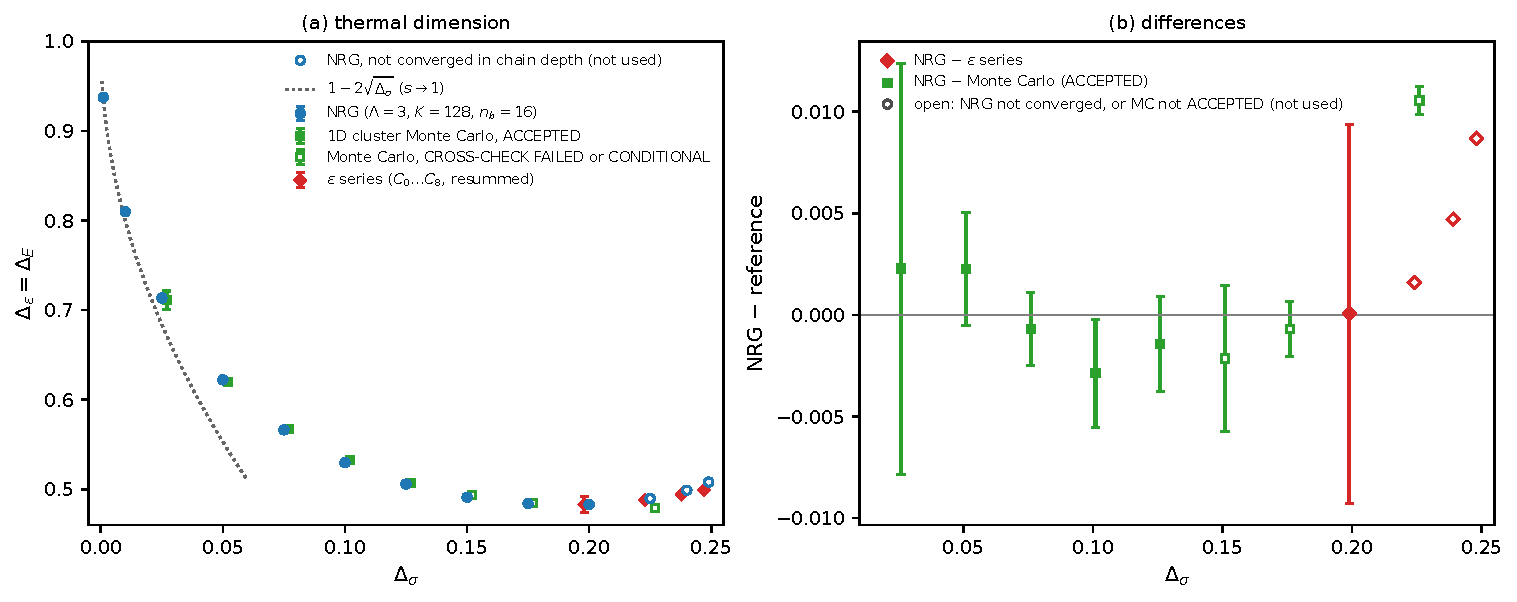
\includegraphics[width=\textwidth]{parts/nrg/figures/fig_checks.pdf}
\caption{(a) $\DE$ against $\Ds$: NRG (filled circles with $\dtot$; open: not converged in chain depth, not used), the project's 1D
cluster Monte Carlo study (filled squares: label ACCEPTED; open: CROSS-CHECK FAILED or CONDITIONAL, which that study does not certify as
infinite-size values; bars $\sigma_{\rm stat}+\sigma_{\rm sys}$, added linearly), the resummed $\varepsilon$ series (diamonds; bars:
spread over Pad\'e approximants, at $\Ds=0.249$ the partial-sum error) and $1-2\sqrt{\Ds}$ near $s=1$. (b) NRG minus reference; bars
are $\dtot$ plus the reference's error, added linearly. Open symbols are not used in any comparison.}\label{nrg:fig:checks}
\end{figure}

What the checks establish:
\begin{itemize}
\item \textbf{The code computes what it claims.} A second implementation written from a physics-only specification
  (Sec.~\ref{nrg:sec:indep}) agrees with the production solver in eight configurations: chain coefficients to better than $\nrgindChain$ (relative, rounding level),
  critical couplings bitwise in $\nrgindAlphaBitwise$ of $\nrgindN$ configurations and to $\nrgindAlpha$ in the others, and $\DE$
  window by window to $\nrgindDE$ wherever its finite differences are reliable. This tests the numerical map, not the estimator.
\item \textbf{Comparison with methods that do not use NRG.} Near $s=1$ the final values reproduce the dual expansion of $\De$ in
  $\sqrt{\Ds}$ through its fifth coefficient (Sec.~\ref{nrg:sec:s1}). At the $\nrgmcAccN$ points where the Monte Carlo study accepts its
  own value they differ from it by at most $\nrgmcAccDiffMax$: within $\sigma_{\rm stat}+\sigma_{\rm sys}+\dtot$ at
  $\nrgmcAccWithinLin$ points and $\nrgmcAccRatioMax$ times that sum at $\Ds=\nrgmcAccDiffMaxAt$. The sum adds a standard deviation, a
  fit-model half-range and an error scale and is only a scale, not a test of statistical consistency. The differences are up to
  $\nrgmcAccStatRatioMax$ Monte Carlo statistical errors and have the same sign at neighboring points, so only the Monte Carlo
  half-range $\sigma_{\rm sys}$ reconciles the two, and the comparison tests the Monte Carlo systematics more than NRG
  (Sec.~\ref{nrg:sec:mc}). At $\Ds=0.2$ the resummed series has a spread of $\nrgserSpreadTwoHundred$ and does not test NRG.
\item \textbf{Near $s=1/2$ the chain is too short.} The flow approaches its fixed point at a rate $\omega\approx\varepsilon\to0$ in
  the RG time $l$. At $\Ds=0.249$ the inverse distance to the series value grows nearly linearly in $l$, with slopes $\nrgslopeEarly$
  to $\nrgslopeLate$, of the size of the one-loop prediction ($\nrgslopePredEarly$ to $\nrgslopePredLate$; Fig.~\ref{nrg:fig:flow}c,
  Sec.~\ref{nrg:sec:approach}). Convergence scans in $K$, $n_b$ or $\Lambda$ at fixed depth cannot reveal this, because once $K$ and
  $n_b\ge12$ are converged the effect depends only on $l$.
\end{itemize}
The errors are error scales built from measured spreads and a few stated judgements (Sec.~\ref{nrg:sec:budget}); they are not standard
deviations. In the text they are quoted with two significant digits; in the tables value(error) follows the PDG rounding (two digits
if the leading digits are 10--35, else one). Bounds in the text (``at most'', ``agree to'', ``below'') are rounded up, so they can
exceed the corresponding table entry by one unit of the last digit. Monte Carlo values and the coefficients $C_7$, $C_8$ are quoted
as their sources give them.

% =====================================================================================================================
\section{The problem and what is known}\label{nrg:sec:model}
% =====================================================================================================================
\subsection{The long-range Ising chain and its thermal dimension}
The ferromagnetic long-range Ising (LRI) chain has spins $S_i=\pm1$ on the sites of a line ($d=1$) and couplings
$J_{ij}\propto1/|i-j|^{1+s}$. It has a finite-temperature transition for $0<s\le1$; the transition is mean-field for $s<1/2$, of
Kosterlitz--Thouless type at $s=1$~\cite{nrg:Kosterlitz1976,nrg:LM01}, and for $1/2<s<1$ its critical point is neither mean-field nor
short-range~\cite{nrg:Fisher1972,nrg:Sak1973}. There the spin field has the exactly known dimension
\begin{equation}
\Ds=\frac{d-s}{2}=\frac{1-s}{2},\qquad s=1-2\Ds,\qquad \varepsilon\equiv2s-d=2s-1=1-4\Ds ,\label{nrg:eq:ds}
\end{equation}
because long-range interactions are not renormalized~\cite{nrg:Sak1973}. The quantity of interest is the dimension of the energy
operator, the leading $\mathbb Z_2$-even scalar,
\begin{equation}
\De=d-\frac1\nu=1-y_t ,\label{nrg:eq:De}
\end{equation}
where $\nu$ is the correlation-length exponent and $y_t=1/\nu$ the renormalization-group (RG) eigenvalue of the temperature.

Two limits are known analytically:
\begin{itemize}
\item \textbf{$s\to1/2^+$ ($\Ds\to1/4$, $\varepsilon\to0$).} The fixed point becomes Gaussian, $\De\to1/2$, and $\De$ has an
  expansion $\De=\sum_nC_n\varepsilon^n$ with $C_0=1/2$, $C_1=-1/6$ and higher coefficients known through $C_8$ (Sec.~\ref{nrg:sec:series},
  Ref.~\cite{nrg:Paper}). The series is asymptotic, but close to $s=1/2$ it is far more precise than any numerical method. The leading
  irrelevant coupling ($\varphi^4$) has the correction exponent $\omega=\varepsilon+O(\varepsilon^2)$, so corrections to scaling
  decay ever more slowly as $s\to1/2$.
\item \textbf{$s\to1^-$ ($\delta\equiv1-s=2\Ds\to0$).} The two lowest $\mathbb Z_2$-even dimensions are
  $\Delta_\pm=1\pm\sqrt{2\delta}+\delta/4+O(\delta^{3/2})$~\cite{nrg:BLMV25,nrg:BLMV26}; the leading term is Kosterlitz's~\cite{nrg:Kosterlitz1976}.
  With $\Delta_-\sim\varphi^2$ the energy operator~\cite{nrg:BLMV25},
  \begin{equation}
  y_t=\sqrt{2\delta}-\frac\delta4+O(\delta^{3/2}),\qquad \omega=\Delta_+-1=\sqrt{2\delta}+\frac\delta4+O(\delta^{3/2}).\label{nrg:eq:s1}
  \end{equation}
  So $\omega\approx y_t$ near $s=1$: both are small, but they are comparable (Sec.~\ref{nrg:sec:depth}). Beyond this order the dual
  description gives $\De$ as a series in $\sqrt{\Ds}$,
  \begin{equation}
  \De=1+\sum_{n\ge1}C^{\rm SR}_n(1)\,\Ds^{n/2},\qquad C^{\rm SR}_1(1)=-2,\quad C^{\rm SR}_2(1)=\tfrac12,\label{nrg:eq:dual}
  \end{equation}
  equivalent to Eq.~\eqref{nrg:eq:s1} through its second term, with $C^{\rm SR}_3(1)$ to $C^{\rm SR}_8(1)$ computed in the accompanying
  paper~\cite{nrg:Paper}; $C^{\rm SR}_3(1)=\frac{39}{16}+2\zeta(2)$, $C^{\rm SR}_4(1)=4-4\zeta(2)-8\zeta(3)$,
  $C^{\rm SR}_5(1)=\frac{11249}{1024}-\frac{361}{16}\zeta(2)+24\zeta(3)+\frac{49}{2}\zeta(4)$ and
  $C^{\rm SR}_6(1)=26-38\zeta(2)+104\zeta(3)-80\zeta(4)-272\zeta(5)+112\zeta(2)\zeta(3)$.
\end{itemize}

\subsection{The spin--boson model}
The spin--boson model without a static bias field describes a two-level system coupled to a bath of harmonic
oscillators~\cite{nrg:Leggett1987}:
\begin{equation}
H=-\frac{\Omega}{2}\,\sigma_x+\sum_j\omega_j\,b_j^\dagger b_j+\frac{\sigma_z}{2}\sum_j\lambda_j\,\big(b_j+b_j^\dagger\big),\qquad
\rho(\omega)\equiv\sum_j\lambda_j^2\,\delta(\omega-\omega_j)=2\alpha\,\omega^{s}\quad(0<\omega\le1).
\label{nrg:eq:H}
\end{equation}
Here $\sigma_{x,z}$ are Pauli matrices, $\Omega$ is the tunneling amplitude (often called $\Delta$ in the literature), $b_j$
annihilates a bath oscillator of frequency
$\omega_j$, $\lambda_j$ is its coupling, $\rho(\omega)$ is the bath spectral density (the convention of Ref.~\cite{nrg:Bulla2003}, equal to
$J(\omega)/\pi$ in Ref.~\cite{nrg:Leggett1987}), $\alpha$ is the dimensionless dissipation strength and $0<s<1$ (``sub-ohmic''). The bath
cutoff frequency is the unit of energy, and $\Omega=0.1$ throughout; universality in $\Omega$ was not tested (Sec.~\ref{nrg:sec:limits}).

For $0<s<1$ the model has a quantum phase transition at a critical coupling $\alpha_c(s,\Omega)$~\cite{nrg:Bulla2003,nrg:Vojta2006}. For
$\alpha<\alpha_c$ (delocalized phase) the ground state is unique; for $\alpha>\alpha_c$ (localized phase) it is twofold degenerate,
the spin being trapped in one of the eigenstates of $\sigma_z$. In the $\sigma_z$ basis the imaginary-time path integral is a classical
Ising chain along the imaginary-time axis, with lattice spacing of order the inverse cutoff~\cite{nrg:Leggett1987,nrg:Vojta2006}: the
tunneling $\Omega$ gives a short-range coupling between neighboring time slices, and integrating out the bath gives a long-range
coupling $\propto\alpha/\tau^{1+s}$, so $\alpha$ plays the role of the inverse temperature. The quantum critical point is therefore in
the universality class of the $d=1$ LRI model with the same $s$: $\langle\sigma_z(\tau)\sigma_z(0)\rangle\propto\tau^{-2\Ds}$ there,
and $\alpha-\alpha_c$, which is $\mathbb Z_2$-even, couples to the energy operator, so its RG eigenvalue is the $y_t$ of
Eq.~\eqref{nrg:eq:De}. The other even coupling, $\Omega$, feeds the same single relevant even direction.

\subsection{The thirteen points}
The study covers the thirteen values of $\Ds$ in Table~\ref{nrg:tab:headline}, chosen for a point-by-point comparison with other methods
of the project. The outer points $\Ds=0.249$ ($s=0.502$) and $0.001$ ($s=0.998$) are the hardest for every method: near $s=1/2$ the
fixed point is almost Gaussian and the approach to it is slow, near $s=1$ the exponent $y_t$ is small.

% =====================================================================================================================
\section{Method: bosonic NRG with an exact \texorpdfstring{$\alpha$}{alpha}-derivative}\label{nrg:sec:method}
% =====================================================================================================================
NRG~\cite{nrg:Wilson1975,nrg:Bulla2008}, extended to bosonic baths in Refs.~\cite{nrg:Bulla2003,nrg:Bulla2005}, solves an impurity coupled to a bath
by mapping the bath onto a chain whose sites carry exponentially decreasing energy scales, and then diagonalizing the chain one site
at a time, keeping only the lowest states. We use the standard formulation; the non-standard elements are the way $y_t$ is extracted
(Secs.~\ref{nrg:sec:tangent}--\ref{nrg:sec:estimator}).

\subsection{Logarithmic discretization}
The bath interval $(0,1]$ is divided into bins $I_m=(\Lambda^{-(m+1)},\Lambda^{-m}]$, $m=0,1,2,\dots$, with a discretization ratio
$\Lambda>1$. Each bin is replaced by a single oscillator $c_m$ that carries the bin's spectral weight at its mean
frequency~\cite{nrg:Bulla2003,nrg:Bulla2005}. With $q=1/\Lambda$, this ``star'' representation has
\begin{equation}
\gamma_m^2=\int_{I_m}\!\rho(\omega)\,d\omega=\frac{2\alpha\,(1-q^{s+1})}{s+1}\,q^{m(s+1)},\qquad
\xi_m=\frac{\int_{I_m}\omega\rho(\omega)\,d\omega}{\gamma_m^2}=\xi_0\,q^m,\qquad \xi_0=\frac{s+1}{s+2}\,\frac{1-q^{s+2}}{1-q^{s+1}},
\label{nrg:eq:star}
\end{equation}
where $\gamma_m$ is the coupling and $\xi_m$ the frequency of oscillator $m$. Every decade of frequency gets the same number of modes,
however low; dropping all other modes of a bin is the approximation of this step, which becomes exact as $\Lambda\to1$.

\subsection{Wilson chain}
An orthogonal change of basis among the $c_m$ (Lanczos tridiagonalization, started from the combination $\sum_m\gamma_mc_m$ that
couples to the spin) maps the star onto a semi-infinite chain:
\begin{equation}
H=-\frac{\Omega}{2}\sigma_x+\frac{\lambda_{\rm tot}}{2}\,\sigma_z\,(b_0+b_0^\dagger)+\sum_{n\ge0}e_n\, b_n^\dagger b_n
+\sum_{n\ge1}t_{n-1}\,(b_{n-1}^\dagger b_n+b_n^\dagger b_{n-1}),\qquad \lambda_{\rm tot}^2=\sum_m\gamma_m^2=\frac{2\alpha}{s+1}.
\label{nrg:eq:chain}
\end{equation}
The spin now couples only to site 0, and each site only to its neighbors; $e_n$ are the on-site energies and $t_n$ the hoppings. The
star has weights $\gamma_m^2\propto(aq)^m$ at the nodes $\xi_0q^m$, with $a=q^s$: this is the orthogonality measure of the little
$q$-Jacobi polynomials $p_n(x;a,1|q)$~\cite{nrg:KLS10}, so the recurrence coefficients are known in closed form. With
\begin{gather}
\mathcal A_n=\frac{(1-aq^{n+1})^2}{(1-aq^{2n+1})(1-aq^{2n+2})},\qquad
\mathcal B_n=\frac{a\,(1-q^n)^2}{(1-aq^{2n})(1-aq^{2n+1})},\nonumber\\
\bar e_n\equiv\Lambda^{n}e_n=\xi_0\,(\mathcal A_n+\mathcal B_n),\qquad
\bar t_n\equiv\Lambda^{n}t_{n-1}=\xi_0\,\sqrt{\mathcal A_{n-1}\mathcal B_n/q}\quad(n\ge1).\label{nrg:eq:coeff}
\end{gather}
(cf.\ also the orthogonal-polynomial chain mappings of Ref.~\cite{nrg:Chin2010}). The code evaluates these closed forms
(\code{lri\_spin.config.chain\_coefficients}); the independent implementation of Sec.~\ref{nrg:sec:indep} obtains the same numbers by a
high-precision Lanczos recursion. Both rescaled coefficients tend to constants, so site $n$ carries the energy scale $\Lambda^{-n}$.
A plain Lanczos recursion on the star is unstable even in multiple-precision arithmetic: without reorthogonalization it loses the
coefficients after 13 sites with 49 digits and after 33 sites with 268 digits (\code{independent\_check/NOTES.md}). The closed form
avoids the problem.

\subsection{Iterative diagonalization and truncation}
Let $H_n$ be the chain~\eqref{nrg:eq:chain} truncated to the sites $0,\dots,n$ and multiplied by $\Lambda^n$. Adding one site is the step
\begin{equation}
H_{n}=\Lambda\,H_{n-1}\otimes\one+\bar e_n\,\one\otimes b^\dagger b
+\bar t_n\,\big(\bar b_{n-1}^\dagger\otimes b+\bar b_{n-1}\otimes b^\dagger\big),\qquad
H_0=-\frac{\Omega}{2}\sigma_x+\bar e_0\,b_0^\dagger b_0+\frac{\lambda_{\rm tot}}{2}\sigma_z\,(b_0+b_0^\dagger),
\label{nrg:eq:step}
\end{equation}
where $\one$ is the identity, $\bar b_{n-1}$ is the annihilation operator of site $n-1$ written in the basis kept at step $n-1$, and
$b$ acts on the new site. The factor $\Lambda$ brings the previous levels to the new energy scale, so the levels of $H_n$ stay of order
one and their evolution with $n$ is an RG flow; its plateaus are fixed points.

Three truncation parameters make each step finite:
\begin{itemize}
\item \textbf{Oscillator cutoff $n_b$.} Each new oscillator keeps its $n_b$ lowest number states. This suffices near the
  delocalized and critical fixed points, where the chain sites hold few bosons~\cite{nrg:Bulla2005}.
\item \textbf{Parity sectors.} The model conserves the parity $P=\sigma_x\,(-1)^{\sum_nb_n^\dagger b_n}$, which implements the Ising
  symmetry. $H_n$ is diagonalized separately in the even and odd sectors, each of dimension at most $Kn_b$.
\item \textbf{Kept states $K$.} In each sector the $K$ lowest eigenstates are kept and the rest discarded. After each step all
  energies are shifted so that the ground state is at zero.
\end{itemize}
Together with $\Lambda$ and the number $N$ of chain sites (the last site sits at energy scale $\Lambda^{-N}$), these parameters
define a finite numerical map from $\alpha$ to a sequence of spectra, which we call the \emph{finite map}. Dense diagonalization costs
of order $(Kn_b)^3$ per sector and site, which limits $K$ and $n_b$.

\subsection{Parity-gap flow and critical coupling}\label{nrg:sec:critical}
The observable is the rescaled parity gap
\begin{equation}
g_n(\alpha)=E^{\rm odd}_{0,n}-E^{\rm even}_{0,n},
\end{equation}
the difference between the lowest levels of $H_n$ in the odd and even sectors. In the delocalized phase $g_n$ flows to its value in
the decoupled chain, where the spin is frozen by $\Omega$ and $g_n$ is the lowest one-boson level; in the localized phase the ground
state becomes degenerate and $g_n\to0$; at $\alpha_c$ it stays on the value of the critical fixed point over an intermediate range
of $n$.

For a chain of $N$ sites, $n=0,\dots,N-1$, the critical coupling of the finite map is located by bisection on the sign of
\begin{equation}
f(\alpha)=g_{N-1}(\alpha)-0.3\,g_{N-1}(0),\label{nrg:eq:bisect}
\end{equation}
the last gap measured against 30\% of the last gap of the decoupled chain ($\alpha=0$) with the same parameters; $f>0$ on the
delocalized side and $f<0$ on the localized side. The rule is:
\begin{itemize}
\item \textbf{Bracket.} Start from $[0.01,2]$; halve the lower end (up to 40 times) until $f>0$; double the upper end until $f<0$,
  never evaluating $\alpha>100$. Without a sign change the item fails.
\item \textbf{Bisection.} At most 48 steps, stopping when the bracket is narrower than $5\times10^{-14}\max(1,|\alpha|)$. A bisection
  that does not reach this width is rejected.
\item \textbf{Result.} $\alpha_c$ is the midpoint of the final bracket. The \emph{terminal residual} is $f(\alpha_c)$.
\end{itemize}
This follows the script of the original study, with two conservative differences: the original evaluated $\alpha$ up to 128 and
accepted an exhausted bisection. The fraction 0.3 is a convention, like the level used to define the crossover
scale in Refs.~\cite{nrg:Bulla2003,nrg:Bulla2005}. The value of $\alpha_c$ is not universal: it depends on $\Lambda$, $K$ and $n_b$
(Fig.~\ref{nrg:fig:alpha}) and enters no result.

\subsection{Exact \texorpdfstring{$\alpha$}{alpha}-derivative of the truncated map}\label{nrg:sec:tangent}
A small detuning $\delta\alpha=\alpha-\alpha_c$ points along the relevant direction of the critical fixed point and grows by a
factor $\Lambda^{y_t}$ per site, so near the fixed point
\begin{equation}
\partial_\alpha g_n\big|_{\alpha_c}\propto\Lambda^{y_tn}.\label{nrg:eq:growth}
\end{equation}
The production code measures this growth without finite differences, by differentiating every step~\eqref{nrg:eq:step} with respect to
$\alpha$, including the change of the kept states. In each parity block write $H=U\,{\rm diag}(E)\,U^{\rm T}$, with kept
eigenvectors $U_k$ (energies $E_k$) and discarded eigenvectors $U_d$ (energies $E_d$), and let $\dot H=\partial_\alpha H$. In the
gauge without rotations among kept states,
\begin{equation}
\dot U_k=U_d\,Z,\qquad Z_{ij}=\frac{\big(U_d^{\rm T}\dot H\,U_k\big)_{ij}}{E_{k,j}-E_{d,i}},\qquad
T=U_k^{\rm T}\dot H\,U_k-\dot E_0\,\one,
\label{nrg:eq:tangent}
\end{equation}
where $\dot E_0$ is the derivative of the ground-state energy (the shift to zero is part of the step). $T$, the derivative of the kept
Hamiltonian, and the derivative of the projected site operator, $\dot{\bar b}=\dot U_k^{\rm T}B\,U_k+U_k^{\rm T}B\,\dot U_k$ with $B$
the site-$n$ annihilation operator in the unrotated product basis, are carried to the next step, where
$\dot H_{n+1}=\Lambda\,T\otimes\one+\bar t_{n+1}(\dot{\bar b}^\dagger\otimes b+{\rm h.c.})$. Only $H_0$ depends on $\alpha$
explicitly, through $\lambda_{\rm tot}\propto\alpha^{1/2}$. The derivative of the gap is $\partial_\alpha g_n=T^{\rm odd}_{00}-T^{\rm
even}_{00}$. This is the exact derivative of the finite map wherever the kept and discarded levels are separated; if the gap between
them falls below $5\times10^{-13}\max(1,|E|)$ the item fails and no record is written. A finite difference in $\alpha$ would instead
turn nonlinear once $\delta\alpha\,\Lambda^{y_tn}$ is no longer small, and lose digits to rounding as $\delta\alpha\to0$.

\subsection{The window audit}\label{nrg:sec:windows}
Near the fixed point, Eq.~\eqref{nrg:eq:growth} gives $\ln|\partial_\alpha g_n|=\kappa+y_t\,n\ln\Lambda$. The window audit, inherited from
the analyzer of the original study, is:
\begin{enumerate}
\item \textbf{Windows.} Windows of $w=\max(12,\lfloor0.13N\rfloor)$ consecutive sites, with first sites from $\max(8,\lfloor0.13N\rfloor)$
  up to (excluding) $\lfloor0.76N\rfloor-w$. A window is skipped if any gap $g_n\le0$ or any $\ln|\partial_\alpha g_n|$ is not finite.
\item \textbf{Fit.} In each window a least-squares line in $n$ is fitted to $\ln|\partial_\alpha g_n|$; its slope divided by $\ln\Lambda$
  is $y_t$, and $\DE=1-y_t$. The \emph{fit residual} is the largest absolute deviation from the line.
\item \textbf{Flatness.} The \emph{relative variation} of the window is $(\max g_n-\min g_n)/|\overline{g_n}|$.
\item \textbf{Quality windows} have relative variation $<0.005$ and fit residual $<0.003$ (inherited conventions). Their number is
  $\nq$, and their $\DE$ values span the \emph{quality range}.
\end{enumerate}
The audit uses no target value of any exponent.

\subsection{The estimate: settled value, plateau and extrapolation}\label{nrg:sec:estimator}
The window values of an item are not constant (Fig.~\ref{nrg:fig:plateau}). Along the chain the flow first approaches the fixed point,
with irrelevant corrections decaying as $e^{-\omega l}$ in the \emph{RG time} $l=n\ln\Lambda$; once the residual detuning has grown
(Sec.~\ref{nrg:sec:depth}) it leaves the fixed point again. The estimate is taken where the flow is closest to the fixed point, by a rule
with three steps (\code{code/analysis/estimator.py}):
\begin{enumerate}
\item \textbf{Settled value.} The \emph{settled window} is the window with the smallest fit residual plus relative variation; its
  $\DE$ is the \emph{settled value}. This is the window the original analyzer reports, stored in every record as \code{selected}.
\item \textbf{Plateau test.} Take the windows whose first site lies within $h=\lceil w/4\rceil$ sites of that of the settled window.
  The largest $|\DE-\text{settled value}|$ among them is the \emph{plateau drift}. A point has a \emph{plateau} if the plateau drift
  of its central item is at most $\tau_{\rm p}=\nrgtau$. Its value is then the settled value, and the plateau drift is its chain-depth
  error.
\item \textbf{Extrapolation}, where there is no plateau. The local exponent
  \begin{equation}
  \Dloc(n)=1-\frac{\ln|\partial_\alpha g_{n+1}|-\ln|\partial_\alpha g_{n-1}|}{2\ln\Lambda}\label{nrg:eq:loc}
  \end{equation}
  is fitted with $\Delta_\infty+A\,e^{-\omega(l-l_0)}$ (free $\Delta_\infty$, $A$, $\omega$; unweighted least squares) on
  $l_{\rm hi}-S\le l\le l_{\rm hi}$ for $S=\nrgspans$, where $l_{\rm hi}$ is the RG time of the last site of the settled window and
  $l_0$ that of the first fitted site. The value is the median of the three $\Delta_\infty$, and the chain-depth error is the larger of
  $|\text{extrapolated}-\text{settled}|$ and the spread of the three fits. Details: a range with fewer than 8 sites is skipped; the
  start values are $\Delta_\infty$ = last point, $A$ = first minus last, $\omega=0.2$; the fit is Levenberg--Marquardt. The
  extrapolation counts as \emph{determined} only if every fit converged with $\omega>0.01$; otherwise it is reported as not
  determined (n.d.), and a point that needs it would stop the analysis.
\end{enumerate}
Every item of a point is evaluated with that point's estimator, so the scans of Sec.~\ref{nrg:sec:budget} compare like with like. The rule
was written on 13 October 2026 and its constants were not varied afterwards (Sec.~\ref{nrg:sec:budget}, App.~\ref{nrg:app:provenance}). It replaces the midpoint of
the quality range used before; App.~\ref{nrg:app:midpoint} explains why and lists the old values.

At $\Ds=0.001$ the rule's own fit ranges lie entirely on the flat plateau, so its extrapolation is not determined (n.d.); the point
has a plateau and is not extrapolated.

\textbf{Classification of the points.} The rule puts each point in one of two classes, \emph{plateau} or \emph{extrapolated}. The eight
points with $\Ds\le0.15$ have a plateau: their plateau drift is at most $\nrgdriftMaxPlateau$ (at $\Ds=\nrgdriftMaxPlateauAt$) and at
most $\nrgdriftMaxLow$ for $\Ds\le0.125$. None of the five points with $\Ds\ge0.175$ has one: their smallest drift is
$\nrgdriftMinNoPlateau$ (at $\Ds=\nrgdriftMinNoPlateauAt$). Every threshold between these two numbers gives the same classification.
The drift grows smoothly with $\Ds$, so the split also depends on $h$ and on the window width $w$, which the rule fixes. At $\Ds=0.15$
the drift is $\nrgdriftHalfOneFifty$ with $h=w/2$ and $\nrgdriftTwentyOneFifty$ with windows of 20 sites, above $\tau_{\rm p}$ in both
cases, so the point would be extrapolated; every point with $\Ds\le0.125$ keeps its plateau (drifts below $\nrgdriftHalfLow$ and
$\nrgdriftTwentyLow$). The values hardly depend on the class: extrapolating at $\Ds=0.15$ would move the value by $\nrgreclassOneFifty$,
windows of 20 sites move its settled value by $\nrgsettledTwentyShiftOneFifty$, and taking the settled value at $0.175$ would move it by
$\nrgreclassOneSeventyFive$, all well inside $\dtot$. At the two final points without a plateau the extrapolation is the value
(Table~\ref{nrg:tab:extrap}).

A third label, \emph{not converged in chain depth}, is not an outcome of the rule. The author assigned it on 13 October 2026 to the
three points closest to $s=1/2$, $\Ds=0.249$, $0.24$ and $0.225$, when the comparison with the $\varepsilon$ series was already known
(App.~\ref{nrg:app:provenance}). The reasons: there $\omega\,l_{\max}\approx61\varepsilon$ is small (Sec.~\ref{nrg:sec:depth}); at
$\Ds=0.249$ the excess over the series decays at a rate of the one-loop size (Sec.~\ref{nrg:sec:approach}); and the excess of the settled
values over the series falls smoothly with $\varepsilon$ (Sec.~\ref{nrg:sec:series}). At $\Ds=0.225$ the rule alone would extrapolate: its
three fits converge, with $\omega=\nrgruleOmTwoTwentyFive$, and give $\nrgruleTwoTwentyFive$ with $\dd=\nrgruleDepthTwoTwentyFive$.
The label there rests on the trend from the two other points and on the Borel--Pad\'e sum of the series; optimal truncation of the
series, $\nrgserOptTwoTwentyFive$, does not exclude the settled value. For the three labeled points the settled value is shown, the
extrapolations are cross-checks only, and no error is quoted. That they ``enter no comparison'' means that no agreement or
disagreement is claimed from their values; the label itself came from a comparison.

\subsection{Cross-check fits (not adopted)}\label{nrg:sec:crosscheck}
The rule's fits end at the settled window and contain no term for the departure from the fixed point, so on a plateau they return the
plateau almost by construction. Two fits that include that departure test the rule from outside (\code{code/analysis/crosscheck.py},
written for the second review round, App.~\ref{nrg:app:provenance}). Neither is adopted, and no value in this note is taken from them. Both
fit $\Dloc(l)$ of the central item with an approach term plus a \emph{detuning term} $A_{\rm d}\,e^{(1-\Delta_\infty)(l-l_{\rm end})}$,
whose growth rate $1-\Delta_\infty=y_t$ is that of the residual detuning (Sec.~\ref{nrg:sec:depth}). Each fit range runs from a start
$l_{\rm a}$ to $l_{\rm end}=l_N-k/y_t$, where $l_N=N\ln\Lambda$ is the end of the chain and $y_t$ is taken from the settled value, so the
last stretch of RG time, where the detuning dominates, is left out. The fits are Levenberg--Marquardt; the result is the median over the
accepted fits, with their range and number $n_{\rm fit}$.
\begin{itemize}
\item \textbf{Late fit.} Approach term $A\,e^{-\omega(l-l_{\rm a})}$; $l_{\rm a}\in\{20,25,30,35\}$ ($\{40,50,60,70\}$ at
  $\Ds=0.001$), $k\in\{8,10,12\}$, at least 10 sites per range; a fit is accepted if its largest residual is below $2\times10^{-6}$
  (below $2\times10^{-5}$ if no fit reaches $2\times10^{-6}$). It is computed at every point and shown for the final points
  (Table~\ref{nrg:tab:budget}).
\item \textbf{Crossover fit.} Approach term $A/(e^{\omega(l-l_0)}-1)$, the one-loop crossover form of Eq.~\eqref{nrg:eq:oneloop} with a
  free $l_0$, or $A\,e^{-\omega(l-l_{\rm a})}$; $l_{\rm a}\in\{13,18,22\}$, $k\in\{12,15\}$, at least 8 sites per range; a fit is
  accepted if its largest residual is below $2\times10^{-5}$ and $0<\omega<2$. It is computed at $\Ds\ge0.2$, where the approach is
  slowest (Tables~\ref{nrg:tab:extrap} and~\ref{nrg:tab:series}).
\end{itemize}
\textbf{The late fit against the rule.} It reproduces the plateau values to $\nrglateMaxLow$ at $0.001\le\Ds\le0.125$, and differs from
the final values by $\nrglateOneFifty$, $\nrglateOneSeventyFive$ and $\nrglateTwoHundred$ at $\Ds=0.15$, $0.175$ and $0.2$. This is
inside $\dd$ except at $\Ds=\nrglateOutside$, where it is $\nrglateOne$ against $\dd=\nrgdepthOne$, far inside $\dtot$. At $\Ds=0.01$
its fitted $\omega=\nrglateOmTen$ agrees with $\sqrt{2\delta}+\delta/4=\nrgnloOmTen$ from Eq.~\eqref{nrg:eq:s1}. At $\Ds=0.2$ it suggests
that the rule's extrapolation, which ends where the detuning already bends $\Dloc$, lies slightly low, by about a tenth of $\dtot$.
The crossover fit is discussed with the $\varepsilon$ series in Sec.~\ref{nrg:sec:series}.

\subsection{Chain depth}\label{nrg:sec:depth}
The bisection stops when its bracket is narrower than $5\times10^{-14}$ (relative), so the critical coupling of the finite map is
located to $\delta\alpha\approx5\times10^{-14}$. This width is at the rounding level of the map: the same item run on 1 and on 2 threads
gives values of $\alpha_c$ that differ by up to $\nrgexRel$, and the two implementations of Sec.~\ref{nrg:sec:indep} differ by up to
$\nrgindAlpha$ (relative), so a narrower bracket would not locate the critical coupling better in double precision. The residual
detuning also grows as $\Lambda^{y_tn}$, and the flow therefore stays near the fixed point only up to
\begin{equation}
n\lesssim n_{\max}\simeq\frac{\ln(1/\delta\alpha)}{y_t\ln\Lambda}\approx\frac{30.6}{y_t\ln\Lambda},\qquad
l\lesssim l_{\max}=n_{\max}\ln\Lambda\approx\frac{30.6}{y_t},\label{nrg:eq:nmax}
\end{equation}
with $30.6=\ln(2\times10^{13})$: the usable RG time is fixed whatever $\Lambda$. The chain lengths follow this estimate: at
$\Lambda=3$, $N=65$ for $s\le0.8$, then $70$, $80$, $90$ and $105$ for $s=0.85$, $0.9$, $0.95$, $0.98$, and $N=250$ at $s=0.998$; for
other $\Lambda$, $N(\Lambda)=N(3)\ln3/\ln\Lambda$. Where $N\approx n_{\max}$ the terminal residual $|f(\alpha_c)|$ is of order 0.1--0.4,
which is expected and not a failure. At $\Ds=0.025$, where $N=90$ and $n_{\max}\approx\nrgnmaxTwentyFive$, the terminal residuals are
$\nrgtermTwentyFiveLo$ to $\nrgtermTwentyFiveHi$; at $\Ds\le0.01$ the chains are clearly shorter than $n_{\max}$ (at $s=0.98$, $N=105$
against $n_{\max}\approx146$) and they are at most $\nrgtermTenMax$ at $\Ds=0.01$ and $\nrgtermOneMax$ at $0.001$ (App.~\ref{nrg:app:items}).

The flow reaches its fixed point within the usable depth only if $\omega\,l_{\max}\approx30.6\,\omega/y_t$ is large. Near $s=1$,
Eq.~\eqref{nrg:eq:s1} gives $\omega/y_t\to1$, so $\omega l_{\max}\approx30$ however small $y_t$ becomes. Near $s=1/2$, $\omega\approx\varepsilon$
and $y_t\approx1/2$, so $\omega l_{\max}\approx61\varepsilon$: about 0.25, 2.4 and 6 at $\Ds=0.249$, $0.24$ and $0.225$. This is why the
plateau is lost as $s\to1/2$ and not as $s\to1$. Extended-precision arithmetic would lengthen $l_{\max}$ in proportion to the number of
digits.

% =====================================================================================================================
\section{Error budget}\label{nrg:sec:budget}
% =====================================================================================================================
For each final point the value is that of Sec.~\ref{nrg:sec:estimator} for the central item. Its error has three components, each computed
with the point's estimator:
\begin{itemize}
\item $\dd$ (chain depth): the plateau drift of the central item; at an extrapolated point, the larger of $|\text{extrapolated}-
  \text{settled}|$ and the spread of the three fits (Sec.~\ref{nrg:sec:estimator}).
\item $\dK$ ($K$ and $n_b$): the spread (maximum minus minimum) over all $\Lambda=3$ items with $K\ge64$ and $n_b\ge10$; at $\Ds\ge0.2$,
  where $n_b=10$ is not converged (Sec.~\ref{nrg:sec:keepnb}), items with $n_b=10$ are left out.
\item $\dL$ (discretization): the larger of two numbers.
  \begin{itemize}
  \item[(a)] The spread over the items at different $\Lambda$, each at the largest $K$ run there, with equal $n_b$ ($16$ at $\Ds\ge0.2$,
    else $10$): $\Lambda=2.5$ and $3$ at $K=128$ at every point; for $\Ds<0.2$ also $\Lambda=4$, run only at $K=64$; and $\Lambda=2$ at
    $K=256$ at $\Ds=0.1$ and $0.05$. The $K$ convergence of $\Lambda=4$ at $K=64$ is assumed, not tested: larger $\Lambda$ needs
    fewer kept states (Sec.~\ref{nrg:sec:lambda}), and at $\Lambda=3$ the values are converged at $K=48$ already (Sec.~\ref{nrg:sec:keepnb}).
  \item[(b)] The shift of the $\Lambda=2.5$ value under its one doubling of $K$, from 64 to 128, at $n_b=10$, the only $n_b$ run at
    $\Lambda=2.5$, $K=64$ (at $\Ds\ge0.2$, $n_b=10$ is not converged).
  \end{itemize}
  Part (b) allows for the untested $K$ convergence at $\Lambda=2.5$. It is the larger part at $\nrgnLambdaKdbl$ of the ten final points,
  so at most points the quoted error is mainly this allowance, not a measured systematic of the central value.
\end{itemize}
The total is the linear sum
\begin{equation}
\dtot=\dd+\dK+\dL,\label{nrg:eq:budget}
\end{equation}
listed in Table~\ref{nrg:tab:budget} and shown in Fig.~\ref{nrg:fig:budget}. The points that are not converged in chain depth have no $\dd$
and no $\dtot$. At $\Ds=0.2$, $\dK$ mostly measures how the extrapolation itself scatters between items (the detuning fits of
Sec.~\ref{nrg:sec:estimator} bring those items within about $2\times10^{-5}$ of each other), so it partly counts $\dd$ twice; this is
conservative.

\textbf{What this error is, and is not.} None of the components is a standard deviation: $\dd$ is a resolution or an extrapolation
length, $\dK$ and $\dL$ are ranges of convergence scans. They are therefore added linearly, not in quadrature. Five choices are
judgements, not measurements:
\begin{itemize}
\item the plateau threshold $\tau_{\rm p}$, the neighborhood $h$ and the window width $w$ (the classification is the same for every
  $\tau_{\rm p}$ between $\nrgdriftMaxPlateau$ and $\nrgdriftMinNoPlateau$; for $h$ and $w$ see Sec.~\ref{nrg:sec:estimator});
\item the fit form, the fit ranges $S$ and the end point $l_{\rm hi}$ of the extrapolation;
\item taking the full extrapolation length as $\dd$ at an extrapolated point;
\item the allowance (b) in $\dL$ for one $K$ doubling at $\Lambda=2.5$;
\item no allowance below $\Lambda=2$: over $2\le\Lambda\le4$ the values agree to $\nrgLspreadPilot$ at the two points where $\Lambda=2$
  is $K$-converged ($\Ds=0.1$, $0.05$), with a small monotone rise with $\Lambda$ far inside the error, but the limit $\Lambda\to1$
  itself is not tested (Sec.~\ref{nrg:sec:lambda}).
\end{itemize}
The window rule of Sec.~\ref{nrg:sec:windows} (width, range, thresholds) is inherited and was not varied in production. Its quality
thresholds do not set the value, because the settled window passes any reasonable threshold. The window width does enter the plateau
test, and with it the class of $\Ds=0.15$, but not its value beyond $2\times10^{-5}$ (Sec.~\ref{nrg:sec:estimator}).

\textbf{When the choices were made.} The rule and its constants were fixed on 13 October 2026, after the NRG data, the earlier
comparisons with the $\varepsilon$ series and the Monte Carlo study, and the reviews' exploratory comparisons had been seen; no
protocol was registered in advance. App.~\ref{nrg:app:provenance} gives the timeline.

\begin{table}[ht]\centering\footnotesize\setlength{\tabcolsep}{4pt}
\caption{Error budget. Columns: estimator (plateau, extrapolated, or settled for the points not converged in chain depth); $\DE$ to six
decimals; the chain-depth error $\dd$, the $K$/$n_b$ spread $\dK$, the discretization error $\dL$ and their linear sum $\dtot$, in
units of $10^{-4}$; the number $\nq$ of quality windows of the central item; the late fit of Sec.~\ref{nrg:sec:crosscheck} minus $\DE$
(cross-check, not adopted; shown for the final points). n.c.: not converged in chain depth.}\label{nrg:tab:budget}
\begin{tabular}{@{}lllrrrrrrl@{}}
\toprule
$\Delta_\sigma$ & estimator & $\Delta_E$ & $10^4\delta_{\rm depth}$ & $10^4\delta_K$ & $10^4\delta_\Lambda$ & $10^4\delta_{\rm tot}$ & $n_q$ & $10^4\,$(late fit $-\Delta_E$) & status\\
\midrule
0.249 & settled & 0.508030 & n.c. & 1.70 & 1.21 & -- & 2 & $--$ & not converged\\
0.24 & settled & 0.498922 & n.c. & 5.12 & 2.54 & -- & 4 & $--$ & not converged\\
0.225 & settled & 0.489668 & n.c. & 2.98 & 6.05 & -- & 9 & $--$ & not converged\\
0.2 & extrapolated & 0.482980 & 4.12 & 2.47 & 0.49 & 7.08 & 15 & $+0.69$ & final\\
0.175 & extrapolated & 0.483900 & 0.86 & 0.80 & 1.80 & 3.46 & 19 & $+0.14$ & final\\
0.15 & plateau & 0.491106 & 0.19 & 0.28 & 0.68 & 1.15 & 21 & $-0.17$ & final\\
0.125 & plateau & 0.505672 & 0.01 & 0.15 & 0.38 & 0.54 & 23 & $-0.00$ & final\\
0.1 & plateau & 0.529608 & 0.02 & 0.05 & 0.27 & 0.33 & 23 & $-0.01$ & final\\
0.075 & plateau & 0.566260 & 0.01 & 0.05 & 0.24 & 0.30 & 28 & $-0.00$ & final\\
0.05 & plateau & 0.622115 & 0.00 & 0.03 & 0.23 & 0.27 & 34 & $-0.00$ & final\\
0.025 & plateau & 0.713422 & 0.01 & 0.02 & 0.26 & 0.29 & 38 & $+0.00$ & final\\
0.01 & plateau & 0.809747 & 0.09 & 0.02 & 0.35 & 0.47 & 41 & $+0.01$ & final\\
0.001 & plateau & 0.937424 & 0.02 & 0.04 & 1.05 & 1.11 & 106 & $+0.03$ & final\\
\bottomrule
\end{tabular}

\end{table}

\begin{figure}[ht]\centering
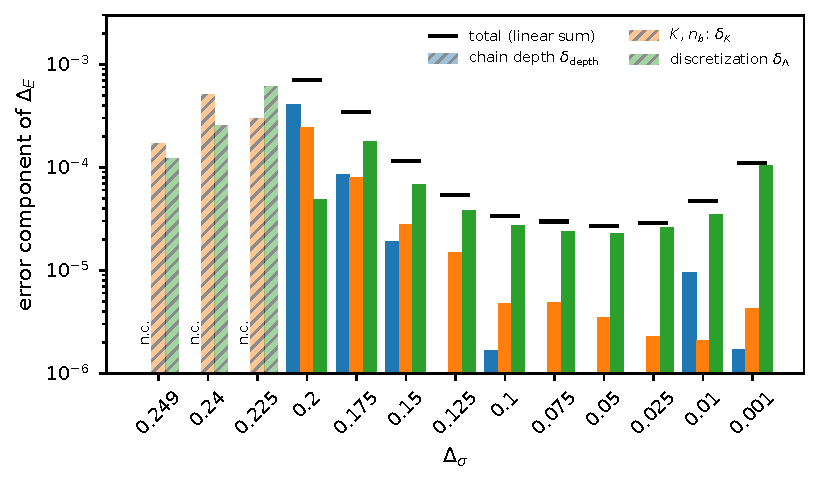
\includegraphics[width=0.72\textwidth]{parts/nrg/figures/fig_error_budget.pdf}
\caption{Components of the error at each $\Ds$ and their linear sum $\dtot$. Hatched: the three points not converged in chain depth,
which have no $\dd$ and no total. At the plateau points $\dL$ dominates, mostly through the $K$-doubling allowance at $\Lambda=2.5$; at
$\Ds=0.2$ the extrapolation length $\dd$ dominates.}\label{nrg:fig:budget}
\end{figure}

% =====================================================================================================================
\section{Software and validation}\label{nrg:sec:software}
% =====================================================================================================================
\subsection{Code}
The solver is the Python package \code{lri\_spin} (\code{code/lri\_spin\_boson\_hpc/src/lri\_spin}; NumPy, SciPy and threadpoolctl;
float64 throughout).
\begin{itemize}
\item \textbf{Backend.} The \code{ordered} backend builds one parity block at a time in the basis order of the reference solver
  (\code{code/lri\_spin\_boson\_hpc/reference/}) and reproduces its flows bitwise and its derivative to rounding (tested). The
  reordered \code{dense} and \code{banded} backends are experimental and were not used.
\item \textbf{Workflows.} The critical search writes checkpoints every 8 sites and persists the bisection state, so an interrupted
  item resumes where it stopped.
\item \textbf{Records.} Each item ends in one result record (App.~\ref{nrg:app:formats}) carrying a SHA-256 checksum and an
  \emph{identity}: the configuration, the kind of run, bracket and tolerances, the SHA-256 of the solver source and the runtime
  (Python, NumPy, SciPy and OpenBLAS versions, BLAS kernel and threading layer). A record from another source or runtime is refused by
  the analysis.
\end{itemize}
Before production Claude Code read the package line by line against the reference solver (App.~\ref{nrg:app:provenance}); no numerical
defect was found and no numerical code was changed.

\subsection{Acceptance gates and tests}
Every result record passed these gates before it was accepted: eigen-residual $\max|HU-UE|\le10^{-8}$ and orthogonality error
$\max|U^{\rm T}U-\one|\le10^{-9}$ at sites $0,1,2$, every 16th site and the last; finite observables and sorted spectra; boson
occupation within $[0,n_b-1]$ and top-level probability (the weight of the highest kept level of the newest oscillator,
$p_{\rm edge}$) within $[0,1]$; for derivatives, a positive gap between kept and discarded levels. Over all $\nrgnItems$ production
records the largest checked eigen-residual is $\nrgmaxEigRes$ and the largest orthogonality error $\nrgmaxOrth$.

The test suite (\code{make test}) has 85 tests. Physics: chain moments, small untruncated spectra against exact diagonalization,
Kronecker products against block operators, reference trajectories, finite differences against the exact derivative. Software:
workflows, record corruption, signals and locks, and the cluster tools of App.~\ref{nrg:app:cluster} (campaign ownership, generations,
lanes, submission against a simulated Slurm, exports, stopping). Before production it passed on a compute node of the cluster for the
final code, in the validation job that issued the receipt \code{inputs/validation\_receipt/receipt.json}. The receipt binds the
solver source to the node runtime: AMD EPYC 7543 nodes, Python 3.13.3, NumPy 2.1.2, SciPy 1.15.2, OpenBLAS 0.3.27/0.3.28 with the
Haswell kernel.

\subsection{Reproducibility across machines}
With the same runtime and thread counts, results are bitwise identical across nodes: a repeated smoke run on a second node reproduced
the first bitwise (App.~\ref{nrg:app:cluster}). Across runtimes, rounding differences are amplified along the relevant direction as
$\Lambda^{y_tn}$: at a \emph{fixed} $\alpha$, late flows of two machines differ, and even two implementations with bitwise identical
$\alpha_c$ (configuration c1 of Sec.~\ref{nrg:sec:indep}) have flows that differ by more than $10^{-8}$ from site $\nrgindDivCone$ on.
Archived values of $\alpha_c$ are therefore not portable, and every item retunes $\alpha_c$ on its own runtime. The critical coupling
itself and the exponent are robust: the production values of $\alpha_c$ reproduce the three couplings archived by the original study
on another machine to $\nrgarchRel$ (relative); the three example items, run on 2 threads, reproduce the $\alpha_c$ of the same items
run on 1 thread bitwise in $\nrgexBitwise$ cases and to $\nrgexRel$ in the third; and the exponents of two implementations agree to
$\nrgindDE$ (Sec.~\ref{nrg:sec:indep}).

% =====================================================================================================================
\section{Production campaigns}\label{nrg:sec:campaigns}
% =====================================================================================================================
All items are critical searches followed by the exact derivative and the window audit, with $\Omega=0.1$, bracket $[0.01,2]$ and
the \code{ordered} backend. Item IDs read \code{ds<$\Ds$>\_L<$\Lambda$>\_K<$K$>\_B<$n_b$>\_N<$N$>}; the example items use
\code{s<$s$>\_L<$\Lambda$>\_K<$K$>\_B<$n_b$>}. Items of the ds13 campaign and the $\Lambda$ campaigns ran on 1 thread if
$Kn_b\le1000$, 2 threads if $Kn_b<1600$ and 4 otherwise; the example items ran on 2 threads, as in the package's example list.
\begin{description}
\item[Example] ($\nrgnItemsExample$ items). The package's example list: $s=0.8$, $0.9$, $0.98$ at $K=64$, $n_b=10$, $\Lambda=3$
  (Table~\ref{nrg:tab:example}). They duplicate three items of the ds13 campaign, which makes them a test of thread-count
  independence (Sec.~\ref{nrg:sec:software}).
\item[ds13] ($\nrgnItemsDs$ items). All thirteen points at $\Lambda=3$ with
  \begin{itemize}
  \item a scan in kept states, $K\in\{48,64,96,128\}$ at $n_b=10$;
  \item a scan in oscillator levels, $n_b\in\{8,12,16\}$ at $K=64$;
  \item $\Lambda\in\{2,4\}$ at $K=64$, $n_b=10$;
  \item the central item $K=128$, $n_b=16$;
  \item extras at the ends: $n_b\in\{20,24\}$ for $\Ds\ge0.2$ and $K\in\{160,192\}$ for $\Ds\le0.05$.
  \end{itemize}
\item[$\Lambda$ pilot] ($\nrgnItemsPilot$ items). $\Ds\in\{0.2,0.1,0.05\}$ at $\Lambda=1.5$ ($K\in\{64,128\}$ at $n_b=10$, $K=64$ at
  $n_b=16$), $\Lambda=2$ ($K=128$) and $\Lambda=2.5$ ($K\in\{64,128\}$), $n_b=10$ unless stated. ($\Lambda=2$, $K=64$ is part of the
  ds13 campaign.)
\item[$\Lambda$ follow-up] ($\nrgnItemsFollowup$ items). $\Lambda=2.5$ at $K\in\{64,128\}$ for the other ten points, plus $K=128$,
  $n_b=16$ for $\Ds\ge0.2$; and $\Lambda=2$ at $K\in\{192,256\}$ for $\Ds\in\{0.2,0.1,0.05\}$.
\end{description}
The runs used $\nrgthreadHours$ thread-hours (sum over items of wall time times threads) on whole cluster nodes. The allocations
summed to $\nrgnodeHours$ node-hours, i.e.\ about $\nrgcoreHoursCharged$ core-hours as charged for 64-core nodes; the longest item
took $\nrglongestItem$\,h, and the production finished within two days including a cluster outage (Table~\ref{nrg:tab:resources} in
App.~\ref{nrg:app:cluster}). The largest peak memory of an item was $\nrgpeakRSS$\,MiB.

\begin{table}[ht]\centering\footnotesize\setlength{\tabcolsep}{4pt}
\caption{The example items ($K=64$, $n_b=10$, $\Lambda=3$, 2 threads): critical coupling, bisection steps, terminal residual
$f(\alpha_c)$, number of quality windows, quality range and settled value. The terminal residuals near $-0.16$ reflect $N\approx n_{\max}$
(Sec.~\ref{nrg:sec:depth}); at $s=0.98$, $N<n_{\max}$.}\label{nrg:tab:example}
\begin{tabular}{llllll}
\toprule
item & $\alpha_c$ & bisection & terminal residual & quality windows & $\Delta_E$ range (settled) \\
\midrule
\texttt{s0.80\_L3\_K64\_B10} & 0.43976978933704 & 46 & $-$0.160 & 23 & [0.52961, 0.53006] (0.52961)\\
\texttt{s0.90\_L3\_K64\_B10} & 0.68913573159160 & 46 & $-$0.159 & 34 & [0.62212, 0.62260] (0.62212)\\
\texttt{s0.98\_L3\_K64\_B10} & 1.08065976531605 & 46 & $+$0.000 & 41 & [0.80946, 0.81013] (0.80975)\\
\bottomrule
\end{tabular}

\end{table}

% =====================================================================================================================
\section{Results}\label{nrg:sec:results}
% =====================================================================================================================
\subsection{The approach to the fixed point}\label{nrg:sec:approach}
Figure~\ref{nrg:fig:flow} shows the local exponent~\eqref{nrg:eq:loc} against the RG time, which is the quantity the estimator works on.
\begin{itemize}
\item \textbf{Plateau ($\Ds=0.1$, panel a).} After the transient, $\Dloc$ is flat over $30\lesssim l\lesssim55$ and the same at
  $\Lambda=2$, $2.5$, $3$ and $4$; the fitted correction exponent is $\omega=\nrgomOneHundred$. The settled window lies on the plateau.
\item \textbf{No plateau ($\Ds=0.2$, panel b).} $\Dloc$ is still falling when the detuning sets in. The settled value,
  $\nrgsetTwoHundred$, is the deepest usable value; the extrapolation (Table~\ref{nrg:tab:extrap}; $\omega=\nrgomTwoHundred$) gives
  $\nrgextTwoHundred$, $\nrgextShiftTwoHundred$ from it, and the extrapolations at $\Lambda=2.5$ and $3$ agree to $\nrgextLamTwoHundred$.
  At $\Ds=0.175$ ($\omega=\nrgomOneSeventyFive$) the shift is $\nrgextShiftOneSeventyFive$.
\item \textbf{Near $s=1/2$ ($\Ds=0.249$, panel c).} At one loop, with the $\varphi^4$ coupling $u$ normalized so that
  $du/dl=\varepsilon u-u^2$ (fixed point $u^*=\varepsilon$), the local dimension of the energy operator is
  $\frac12-\frac\varepsilon2+\frac u3$; the factor $\frac13=(\mathcal N+2)/(\mathcal N+8)$ is that of the Ising case $\mathcal N=1$
  of the O($\mathcal N$) model~\cite{nrg:Fisher1972}, and at $u^*$ it gives $\De=\frac12-\frac\varepsilon6$. A strong bare coupling,
  $u\to\infty$ at some RG time $l_0$, then gives
  \begin{equation}
  \Dloc-\De=\frac{\varepsilon/3}{e^{\varepsilon(l-l_0)}-1},\qquad \frac1{\Dloc-\De}=\frac3\varepsilon\big(e^{\varepsilon(l-l_0)}-1\big),
  \label{nrg:eq:oneloop}
  \end{equation}
  if $\Dloc$ follows the running coupling. The inverse excess thus grows with local slope $3e^{\varepsilon(l-l_0)}$, which tends to 3
  as $\varepsilon(l-l_0)\to0$. With the series value $\De=\nrgserTwoFortyNine$ the measured inverse excess grows nearly linearly in $l$
  at every $K$, $n_b$ and $\Lambda$ shown, with slope $\nrgslopeEarly$ for $15\le l\le25$, $\nrgslopeMid$ over $20\le l\le45$ and
  $\nrgslopeLate$ for $38\le l\le48$. Inferring $l_0$ from the data at $20\le l\le40$ gives $l_0=\nrglzeroLo$ to $\nrglzeroHi$, for
  which Eq.~\eqref{nrg:eq:oneloop} predicts local slopes $\nrgslopePredEarly$ at $l=20$ and $\nrgslopePredLate$ at $l=43$. The measured
  slopes are 10--20\% lower and rise with $l$ as predicted. Terms of higher order in $u$, largest early in the flow where $u$ is
  largest, could account for the difference, but we have not shown that. The test is semi-quantitative: it shows an approach of the
  one-loop kind, at a rate set by $\varepsilon$, not a precise coefficient. At $\Ds=0.249$, $0.24$ and $0.225$ the window $\DE$ still changes by $\nrgdriftSiteTwoFortyNine$,
  $\nrgdriftSiteTwoForty$ and $\nrgdriftSiteTwoTwentyFive$ per site at the settled window. Single-exponential fits give
  $\omega=\nrgomTwoFortyNine$, $\nrgomTwoForty$ and $\nrgomTwoTwentyFive$, which approach $\varepsilon$ ($0.004$, $0.04$, $0.1$) only at the
  largest $\varepsilon$, since an exponential cannot represent a $1/l$ approach, and the three fits scatter by up to
  $\nrgextSpreadTwoTwentyFive$ (Table~\ref{nrg:tab:extrap}). The data do not determine the fixed-point value at these
  points to the precision of the others: they are \emph{not converged in chain depth}. A scan in $K$, $n_b$ or $\Lambda$ at fixed
  $l_{\max}$ cannot reveal this, because once $K$ is converged and $n_b\ge12$ the effect depends only on $l$ ($n_b=8$ and $10$ are
  off by up to $\nrgnbEight$ and $\nrgnbTen$ near $s=1/2$, Sec.~\ref{nrg:sec:keepnb}).
\item \textbf{Near $s=1$ ($\Ds=0.001$, panel d).} $\Dloc$ rises to a long plateau ($75\lesssim l\lesssim120$), as Eq.~\eqref{nrg:eq:nmax}
  allows. At the $10^{-4}$ level the plateau depends on the truncation away from $\Lambda=3$: at $\Lambda=2.5$ it moves by
  $\nrgKdblOne$ between $K=64$ and $128$, at $\Lambda=4$ ($K=64$) it overshoots by about $10^{-4}$ before settling, and at $\Lambda=2$,
  $K=64$ is far from converged ($\nrgLtwoOne$). At the largest $K$ run the values at $\Lambda=2.5$, $3$ and $4$ agree to $\nrgLspreadOne$,
  but at $\Lambda=2.5$ that is a single doubling. The
  plateau value is therefore ambiguous at the $10^{-4}$ level; the budget carries this through the $K$-doubling allowance, which gives
  $\dL=\nrgKdblOne$ at this point (Sec.~\ref{nrg:sec:budget}).
\end{itemize}

\begin{figure}[ht]\centering
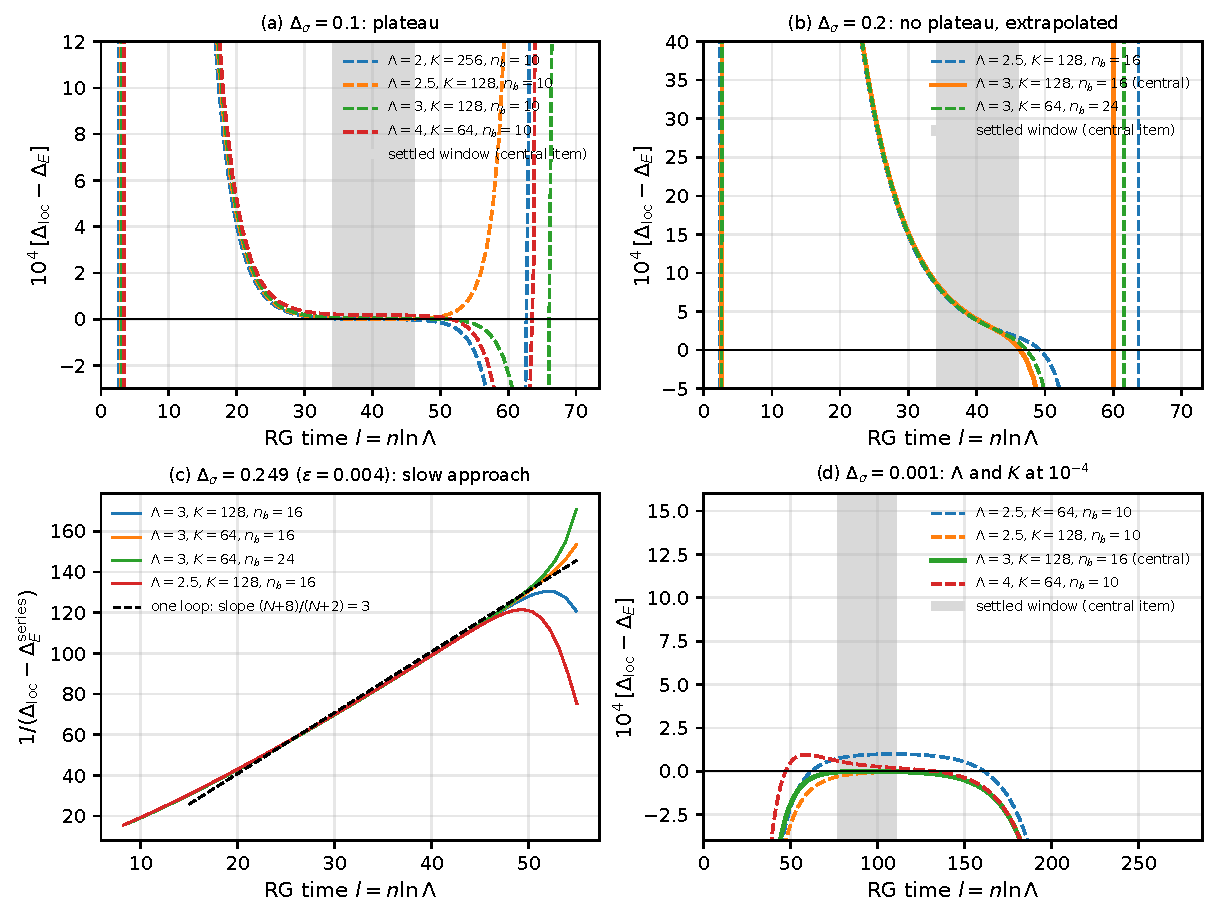
\includegraphics[width=0.95\textwidth]{parts/nrg/figures/fig_flow.pdf}
\caption{Local exponent $\Dloc$, Eq.~\eqref{nrg:eq:loc}, against the RG time $l=n\ln\Lambda$. (a), (b), (d): $10^4\,(\Dloc-\DE)$ relative to
the final value; gray band: the settled window of the central item. (a) $\Ds=0.1$, items at four values of $\Lambda$, each at the
largest $K$ run (at $\Lambda=4$ only $K=64$): a common plateau. (b) $\Ds=0.2$: no plateau; the zero line is the extrapolated value. (d)
$\Ds=0.001$: $\Lambda$ and $K$ at the $10^{-4}$ level. (c) $\Ds=0.249$: inverse distance to the $\varepsilon$-series value against $l$,
for four truncations; dashed: slope 3, the one-loop value for $\varepsilon(l-l_0)\to0$ (Eq.~\eqref{nrg:eq:oneloop}).}\label{nrg:fig:flow}
\end{figure}

\begin{table}[ht]\centering\scriptsize\setlength{\tabcolsep}{2.5pt}
\caption{The points without a plateau (central items). Settled value; plateau drift; change of the window $\DE$ per site at the settled
window; the three fitted $\Delta_\infty$ and $\omega$ for $S=30,25,20$; their median (the extrapolated value). At $\Ds=0.2$ and $0.175$
the median is the final value. Last column: the crossover fit of Sec.~\ref{nrg:sec:crosscheck} (median, number $n_{\rm fit}$ of accepted
fits), computed at $\Ds\ge0.2$ only; a cross-check, not adopted. $^\ast$Not converged in chain depth: cross-check only, not
used.}\label{nrg:tab:extrap}
\begin{tabular}{@{}llllllll@{}}
\toprule
 & & & & \multicolumn{3}{c}{the rule (Sec.~\ref{nrg:sec:estimator})} & cross-check, not adopted\\
\cmidrule(lr){5-7}\cmidrule(lr){8-8}
$\Delta_\sigma$ & settled & drift & per site & fits $\Delta_\infty$ ($S=30,25,20$) & $\omega$ & median & crossover fit ($n_{\rm fit}$)\\
\midrule
0.249$^\ast$ & 0.508030 & $8\times10^{-4}$ & $-3\times10^{-4}$ & 0.50496, 0.50463, 0.50463 & 0.068, 0.064, 0.064 & 0.504628 & 0.50209 (6)\\
0.24$^\ast$ & 0.498922 & $7\times10^{-4}$ & $-2\times10^{-4}$ & 0.49670, 0.49673, 0.49704 & 0.078, 0.079, 0.088 & 0.496734 & 0.49460 (6)\\
0.225$^\ast$ & 0.489668 & $6\times10^{-4}$ & $-2\times10^{-4}$ & 0.48804, 0.48753, 0.48668 & 0.092, 0.078, 0.059 & 0.487529 & 0.48810 (7)\\
0.2 & 0.483392 & $2\times10^{-4}$ & $-7\times10^{-5}$ & 0.48305, 0.48298, 0.48291 & 0.151, 0.142, 0.130 & 0.482980 & 0.48305 (9)\\
0.175 & 0.483986 & $8\times10^{-5}$ & $-2\times10^{-5}$ & 0.48391, 0.48390, 0.48389 & 0.205, 0.199, 0.190 & 0.483900 & --\\
\bottomrule
\end{tabular}

\end{table}

\subsection{Convergence in kept states and oscillator levels}\label{nrg:sec:keepnb}
Table~\ref{nrg:tab:keepnb} and Fig.~\ref{nrg:fig:keepnb} show the deviation of every $\Lambda=3$ item from the central value.
\begin{itemize}
\item \textbf{Kept states.} The estimates are converged at $K=48$ already: for $\Ds\le0.125$ the spread over $K$ is at most
  $\nrgkeepSpread$.
\item \textbf{Oscillator levels.} $n_b$ matters mainly near $s=1/2$, where $n_b=8$ is off by up to $\nrgnbEight$ and $n_b=10$ by up to
  $\nrgnbTen$, while at the final points all items with $n_b\ge12$ (and $K\ge64$) agree with the central value to $\nrgnbTwelve$.
\item \textbf{Top-level probability.} $p_{\rm edge}$ is the weight of the highest level, $n_b-1$, of the newest oscillator in the
  ground state, evaluated at every site of the critical flow; App.~\ref{nrg:app:items} lists its maximum over the chain. That maximum is
  reached at the last sites, where the flow leaves the fixed point, and depends on the side it leaves to: for the items with
  $n_b\ge12$ its median is $\nrgedgeNegMed$ when the flow ends toward the localized phase (negative terminal residual; the bosons are
  displaced there) and $\nrgedgePosMed$ when it ends toward the delocalized phase. This is why it changes by many decades between
  items that differ only in $K$. For $n_b\ge12$ it is at most $\nrgedgeMax$, at most $\nrgedgeCentralMax$ for the central items, and
  below $\nrgedgeMaxLow$ at $\Ds\le0.15$. It is largest near $s=1/2$, where the critical fixed point holds the most bosons.
\end{itemize}

\begin{table}[ht]\centering\scriptsize\setlength{\tabcolsep}{3.5pt}
\caption{Deviation $10^4\,[\DE(K,n_b)-\DE^{\rm central}]$ at $\Lambda=3$ (central: $K=128$, $n_b=16$), each item evaluated with its
point's estimator. In the scan over $K$, the offsets at $\Ds\ge0.2$ come from $n_b=10$, not from $K$. Empty cells were not
run.}\label{nrg:tab:keepnb}
\begin{tabular}{lrrrrrrrrrrrr}
\toprule
 & \multicolumn{6}{c}{$K$ scan ($n_b=10$)} & \multicolumn{6}{c}{$n_b$ scan ($K=64$)}\\
\cmidrule(lr){2-7}\cmidrule(lr){8-13}
$\Delta_\sigma$ & $K{=}48$ & $K{=}64$ & $K{=}96$ & $K{=}128$ & $K{=}160$ & $K{=}192$ & $n_b{=}8$ & $n_b{=}10$ & $n_b{=}12$ & $n_b{=}16$ & $n_b{=}20$ & $n_b{=}24$\\
\midrule
0.249 & $+$10.66 & $+$8.88 & $+$10.28 & $+$10.92 &  &  & $+$94.49 & $+$8.88 & $+$1.08 & $-$0.30 & $+$1.24 & $-$0.45\\
0.24 & $+$7.03 & $+$6.80 & $+$10.23 & $+$7.21 &  &  & $+$89.86 & $+$6.80 & $+$3.00 & $+$5.12 & $+$0.70 & $+$3.32\\
0.225 & $+$2.43 & $+$2.12 & $+$4.70 & $+$4.34 &  &  & $+$65.41 & $+$2.12 & $+$0.20 & $+$0.28 & $+$1.88 & $-$1.10\\
0.2 & $+$2.07 & $+$2.68 & $+$3.46 & $+$3.15 &  &  & $+$33.99 & $+$2.68 & $+$1.84 & $+$1.48 & $-$0.63 & $-$0.15\\
0.175 & $+$0.81 & $+$0.42 & $+$0.80 & $+$0.65 &  &  & $+$16.97 & $+$0.42 & $+$0.20 & $+$0.22 &  & \\
0.15 & $+$0.21 & $+$0.21 & $+$0.15 & $+$0.17 &  &  & $+$9.45 & $+$0.21 & $-$0.07 & $-$0.07 &  & \\
0.125 & $+$0.15 & $+$0.15 & $+$0.13 & $+$0.10 &  &  & $+$5.86 & $+$0.15 & $+$0.03 & $+$0.03 &  & \\
0.1 & $+$0.08 & $+$0.05 & $+$0.05 & $+$0.04 &  &  & $+$3.90 & $+$0.05 & $+$0.01 & $+$0.03 &  & \\
0.075 & $+$0.06 & $+$0.05 & $+$0.03 & $+$0.03 &  &  & $+$2.86 & $+$0.05 & $+$0.02 & $+$0.02 &  & \\
0.05 & $+$0.05 & $+$0.03 & $+$0.02 & $+$0.02 & $+$0.01 & $+$0.01 & $+$2.33 & $+$0.03 & $+$0.01 & $+$0.02 &  & \\
0.025 & $+$0.04 & $+$0.02 & $+$0.02 & $+$0.01 & $+$0.01 & $+$0.01 & $+$2.26 & $+$0.02 & $+$0.01 & $+$0.01 &  & \\
0.01 & $+$0.03 & $+$0.02 & $+$0.02 & $+$0.02 & $+$0.01 & $+$0.01 & $+$2.83 & $+$0.02 & $+$0.01 & $+$0.01 &  & \\
0.001 & $+$0.04 & $+$0.04 & $+$0.04 & $+$0.04 & $+$0.03 & $+$0.01 & $+$7.08 & $+$0.04 & $+$0.00 & $+$0.00 &  & \\
\bottomrule
\end{tabular}

\end{table}

\begin{figure}[ht]\centering
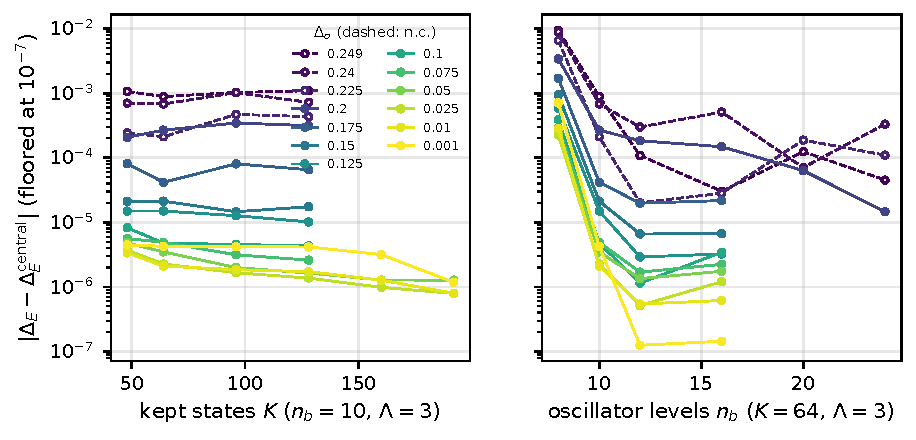
\includegraphics[width=0.92\textwidth]{parts/nrg/figures/fig_keep_nb.pdf}
\caption{$|\DE-\DE^{\rm central}|$ against $K$ (left, $n_b=10$) and $n_b$ (right, $K=64$) at $\Lambda=3$; zero deviations are drawn at
$10^{-7}$. Flat curves mean converged. Dashed: the three points not converged in chain depth. In the left panel the level of the
$\Ds\ge0.2$ curves is set by $n_b=10$.}\label{nrg:fig:keepnb}
\end{figure}

\subsection{Dependence on the discretization \texorpdfstring{$\Lambda$}{Lambda}}\label{nrg:sec:lambda}
The chain length is scaled as $N\propto1/\ln\Lambda$, so all items of a point reach the same RG time. The $\Lambda$ studies separate
truncation from discretization (Tables~\ref{nrg:tab:lambda} and~\ref{nrg:tab:lshift}, Fig.~\ref{nrg:fig:lambda}):
\begin{itemize}
\item \textbf{Smaller $\Lambda$ needs many more kept states.} At $\Lambda=1.5$, going from $K=64$ to $128$ moves $\DE$ by
  $\nrgLonefiveMove$, and $K=128$ is still $\nrgLonefiveOff$ away from the converged $\Lambda=2$ value; raising $n_b$ to 16 changes
  $\DE$ by only $\nrgLonefiveNb$. At $\Lambda=2$, $K=192$ and $256$ agree to $\nrgLtwoKconv$. At $\Lambda=2.5$, $K=64$ and $128$ (one
  doubling) agree to $\nrgLtwofiveKconv$ for $0.01\le\Ds\le0.15$, to $\nrgKdblOne$ at $0.001$, and differ by up to $\nrgLtwofiveKconvHigh$
  at the final points with $\Ds\ge0.175$ (up to $\nrgLtwofiveKconvNc$ at the points not converged in chain depth). At $\Lambda=2$, $K=64$ is not converged: it lies $\nrgLtwoKsixfourSmall$ above $\Lambda=3$ at $\Ds\le0.05$.
\item \textbf{A small $\Lambda$ dependence, far inside the error.} At the largest $K$ run at each $\Lambda$ (at $\Lambda=4$ only
  $K=64$, whose convergence is assumed), the plateau values at $\Lambda=2$, $2.5$, $3$ and $4$ agree to $\nrgLspreadPilot$ at $\Ds=0.1$ and $0.05$, and rise monotonically with $\Lambda$: relative to $\Lambda=3$, $\Lambda=2$,
  $2.5$ and $4$ lie at $\nrgLtwoOneHundred$, $\nrgLtwofiveOneHundred$ and $\nrgLfourOneHundred$ at $\Ds=0.1$, and at $\nrgLtwoFifty$,
  $\nrgLtwofiveFifty$ and $\nrgLfourFifty$ at $0.05$. Extended to $\Lambda\to1$ this would put the $\Lambda=3$ value a few $10^{-6}$ above
  the limit, far below $\dtot$. Over $\Lambda=2.5$--$4$ the largest spread at a plateau point is $\nrgLspreadMax$ (at
  $\Ds=\nrgLspreadMaxAt$, set by $\Lambda=4$). How many kept states the limit $\Lambda\to1$ needs was not determined, and the limit
  is not tested.
\item \textbf{At $\Ds=0.2$} only $\Lambda=2.5$ and $3$ were run with the converged $n_b=16$; their extrapolations agree to
  $\nrgextLamTwoHundred$. At $n_b=10$ the extrapolated values spread by $\nrgLtenSpreadTwoHundred$ over $\Lambda=2$--$4$
  (Fig.~\ref{nrg:fig:lambda}). We attribute this to an interplay of $\Lambda$ with the $n_b=10$ truncation (the $\Lambda=2.5$ minus
  $\Lambda=3$ difference changes sign between $n_b=10$ and $16$), but that is inferred, not measured; it is within $\dtot$ only through
  the large $\dd$.
\end{itemize}
An earlier version of this note reported that $\DE$ rises as $\Lambda$ decreases and covered the continuum limit with twice the
$\Lambda=2.5$ shift. Both came from the midpoint estimator: the window rule counts sites while the chain length scales as
$1/\ln\Lambda$, so smaller $\Lambda$ admitted a larger share of transient windows (App.~\ref{nrg:app:midpoint}).

\begin{table}[ht]\centering\scriptsize
\caption{The $\Lambda$ study at three points ($n_b=10$ unless stated): $\DE$ with this note's estimator (plateau value at $\Ds=0.1$,
$0.05$; extrapolated at $0.2$), the superseded midpoint with its half-width, and $\alpha_c$. $N$ is scaled with $\Lambda$ so that the
infrared scale $\Lambda^{-N}$ is fixed. At $\Lambda=1.5$ no item is converged in $K$.}\label{nrg:tab:lambda}
\begin{tabular}{llllllll}
\toprule
$\Delta_\sigma$ & $\Lambda$ & $K$ & $n_b$ & $N$ & $\Delta_E$ (this note) & old midpoint (half-width) & $\alpha_c$ \\
\midrule
0.2 & 1.5 & 64 & 10 & 176 & 0.536299 & 0.53659 (0.00036) & 0.1626225790\\
0.2 & 1.5 & 64 & 16 & 176 & 0.536300 & 0.53660 (0.00036) & 0.1626210299\\
0.2 & 1.5 & 128 & 10 & 176 & 0.507038 & 0.50754 (0.00102) & 0.1603705735\\
0.2 & 2 & 64 & 10 & 103 & 0.484078 & 0.48534 (0.00177) & 0.1676281822\\
0.2 & 2 & 128 & 10 & 103 & 0.483021 & 0.48471 (0.00165) & 0.1676098637\\
0.2 & 2 & 192 & 10 & 103 & 0.483061 & 0.48448 (0.00193) & 0.1676082707\\
0.2 & 2 & 256 & 10 & 103 & 0.483014 & 0.48449 (0.00188) & 0.1676081346\\
0.2 & 2.5 & 64 & 10 & 78 & 0.483221 & 0.48426 (0.00131) & 0.1761692489\\
0.2 & 2.5 & 128 & 10 & 78 & 0.483173 & 0.48440 (0.00101) & 0.1761670918\\
0.2 & 3 & 64 & 10 & 65 & 0.483248 & 0.48404 (0.00063) & 0.1847222031\\
0.2 & 3 & 128 & 10 & 65 & 0.483295 & 0.48406 (0.00061) & 0.1847217711\\
0.2 & 4 & 64 & 10 & 52 & 0.483381 & 0.48401 (0.00034) & 0.2008115424\\
\midrule
0.1 & 1.5 & 64 & 10 & 176 & 0.567059 & 0.56714 (0.00019) & 0.3786792319\\
0.1 & 1.5 & 64 & 16 & 176 & 0.567059 & 0.56714 (0.00019) & 0.3786839607\\
0.1 & 1.5 & 128 & 10 & 176 & 0.539196 & 0.53968 (0.00049) & 0.3733064368\\
0.1 & 2 & 64 & 10 & 103 & 0.529796 & 0.53042 (0.00063) & 0.3936704020\\
0.1 & 2 & 128 & 10 & 103 & 0.529631 & 0.53025 (0.00063) & 0.3936438035\\
0.1 & 2 & 192 & 10 & 103 & 0.529613 & 0.53024 (0.00063) & 0.3936429089\\
0.1 & 2 & 256 & 10 & 103 & 0.529609 & 0.53023 (0.00064) & 0.3936426886\\
0.1 & 2.5 & 64 & 10 & 78 & 0.529637 & 0.53010 (0.00046) & 0.4167902745\\
0.1 & 2.5 & 128 & 10 & 78 & 0.529610 & 0.53007 (0.00046) & 0.4167874486\\
0.1 & 3 & 64 & 10 & 65 & 0.529613 & 0.52984 (0.00022) & 0.4397697893\\
0.1 & 3 & 128 & 10 & 65 & 0.529612 & 0.52984 (0.00023) & 0.4397694449\\
0.1 & 4 & 64 & 10 & 52 & 0.529628 & 0.52981 (0.00018) & 0.4825812310\\
\midrule
0.05 & 1.5 & 64 & 10 & 217 & 0.670692 & 0.67093 (0.00026) & 0.5909590331\\
0.05 & 1.5 & 64 & 16 & 217 & 0.670693 & 0.67092 (0.00026) & 0.5909603112\\
0.05 & 1.5 & 128 & 10 & 217 & 0.630353 & 0.63061 (0.00026) & 0.5780543351\\
0.05 & 2 & 64 & 10 & 127 & 0.622300 & 0.62262 (0.00032) & 0.6120267877\\
0.05 & 2 & 128 & 10 & 127 & 0.622125 & 0.62241 (0.00036) & 0.6119924970\\
0.05 & 2 & 192 & 10 & 127 & 0.622119 & 0.62244 (0.00033) & 0.6119916485\\
0.05 & 2 & 256 & 10 & 127 & 0.622116 & 0.62242 (0.00034) & 0.6119911289\\
0.05 & 2.5 & 64 & 10 & 96 & 0.622139 & 0.62240 (0.00026) & 0.6507599139\\
0.05 & 2.5 & 128 & 10 & 96 & 0.622116 & 0.62235 (0.00029) & 0.6507542509\\
0.05 & 3 & 64 & 10 & 80 & 0.622119 & 0.62236 (0.00024) & 0.6891357316\\
0.05 & 3 & 128 & 10 & 80 & 0.622117 & 0.62236 (0.00024) & 0.6891354544\\
0.05 & 3 & 192 & 10 & 80 & 0.622117 & 0.62236 (0.00024) & 0.6891353149\\
0.05 & 4 & 64 & 10 & 63 & 0.622122 & 0.62223 (0.00013) & 0.7603342269\\
\bottomrule
\end{tabular}

\end{table}

\begin{table}[ht]\centering\scriptsize
\caption{$\Lambda$ and $K$ shifts at all thirteen points, in units of $10^{-4}$, relative to $\Lambda=3$ at the same $K$ and $n_b$
($\Lambda=2.5$ uses $n_b=16$ for $\Ds\ge0.2$, else $10$). The $\Lambda=2$, $K=64$ column is not converged in $K$. Last columns: the $K$
doubling at $\Lambda=2.5$ ($n_b=10$) and the number of quality windows of the $\Lambda=2.5$, $K=128$, $n_b=10$ item.}\label{nrg:tab:lshift}
\begin{tabular}{llllll}
\toprule
 & \multicolumn{3}{c}{$10^4\times$ shift relative to $\Lambda=3$} & \multicolumn{2}{c}{at $\Lambda=2.5$}\\
\cmidrule(lr){2-4}\cmidrule(lr){5-6}
$\Delta_\sigma$ & $\Lambda{=}2$, $K{=}64$ & $\Lambda{=}2.5$, $K{=}128$ & $\Lambda{=}4$, $K{=}64$ & $10^4\times(K{=}64$ minus $K{=}128)$ & $n_q$\\
\midrule
0.249 & $+$41.37 & $+$1.21 & $+$17.22 & $+$0.88 & 13\\
0.24 & $+$34.03 & $+$0.71 & $+$16.43 & $+$2.54 & 13\\
0.225 & $+$19.17 & $+$2.29 & $+$10.71 & $+$6.05 & 17\\
0.2 & $+$8.30 & $+$0.18 & $+$1.33 & $+$0.49 & 22\\
0.175 & $+$3.71 & $-$0.53 & $+$1.50 & $+$1.55 & 25\\
0.15 & $+$2.38 & $-$0.10 & $+$0.54 & $+$0.67 & 28\\
0.125 & $+$1.90 & $-$0.07 & $+$0.23 & $+$0.38 & 31\\
0.1 & $+$1.84 & $-$0.02 & $+$0.15 & $+$0.27 & 32\\
0.075 & $+$1.75 & $-$0.02 & $+$0.06 & $+$0.24 & 36\\
0.05 & $+$1.81 & $-$0.01 & $+$0.03 & $+$0.23 & 43\\
0.025 & $+$1.62 & $-$0.01 & $+$0.03 & $+$0.26 & 47\\
0.01 & $+$2.02 & $-$0.00 & $+$0.06 & $+$0.35 & 49\\
0.001 & $+$5.63 & $-$0.11 & $+$0.12 & $+$1.05 & 126\\
\bottomrule
\end{tabular}

\end{table}

\begin{figure}[ht]\centering
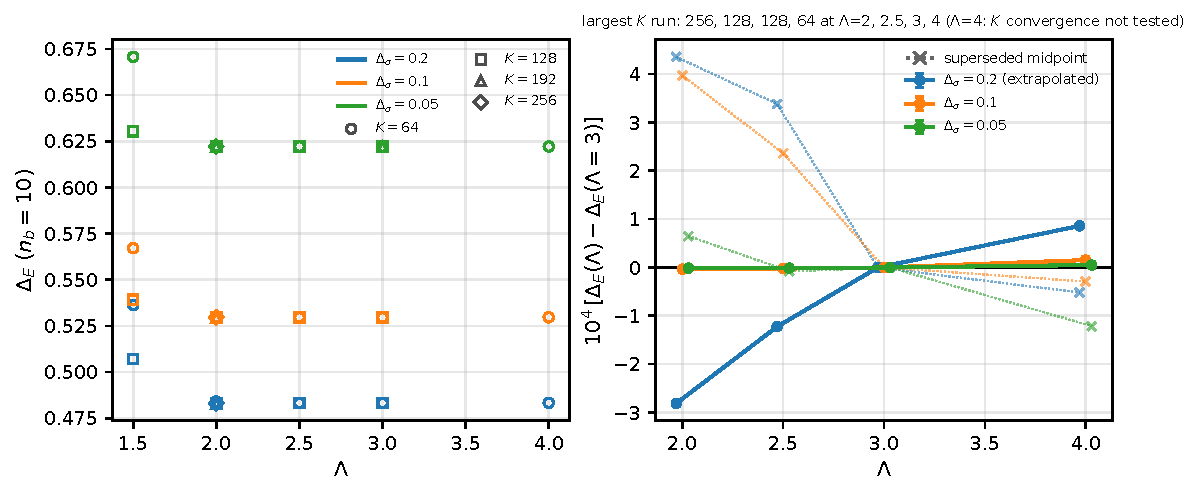
\includegraphics[width=0.95\textwidth]{parts/nrg/figures/fig_lambda.pdf}
\caption{Left: $\DE$ against $\Lambda$ for all $K$ at $n_b=10$ (open symbols by $K$, color by $\Ds$); at $\Lambda=1.5$ no item is
converged in $K$. Right: $K$-converged items relative to $\Lambda=3$ with this note's estimator (bars: plateau drift) and, dotted, the
superseded midpoints, whose apparent $\Lambda$ dependence is an artifact of the window rule.}\label{nrg:fig:lambda}
\end{figure}

\begin{figure}[ht]\centering
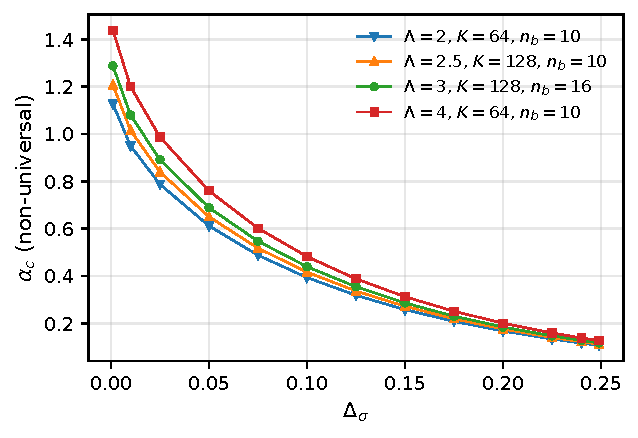
\includegraphics[width=0.6\textwidth]{parts/nrg/figures/fig_alpha_c.pdf}
\caption{The critical coupling is not universal: it depends on $\Lambda$ and weakly on $K$ and $n_b$. It enters no
result.}\label{nrg:fig:alpha}
\end{figure}

\subsection{The final table}\label{nrg:sec:final}
Table~\ref{nrg:tab:headline} gives the final values and Table~\ref{nrg:tab:budget} their errors. Starting from the Gaussian value $1/2$ at
$s=1/2$, $\De$ first decreases (the $\varepsilon$ series at $\Ds\ge0.2$), passes through a shallow minimum of about $\nrgDEmin$ near
$\Ds=\nrgDEminAt$, and rises toward 1 as $s\to1$. The window audits of three central items are shown in Fig.~\ref{nrg:fig:plateau}. The
number of quality windows falls from $\nrgnqOne$ at $\Ds=0.001$ to $\nrgnqTwoFortyNine$ at $\Ds=0.249$ (Table~\ref{nrg:tab:budget}).

\begin{figure}[ht]\centering
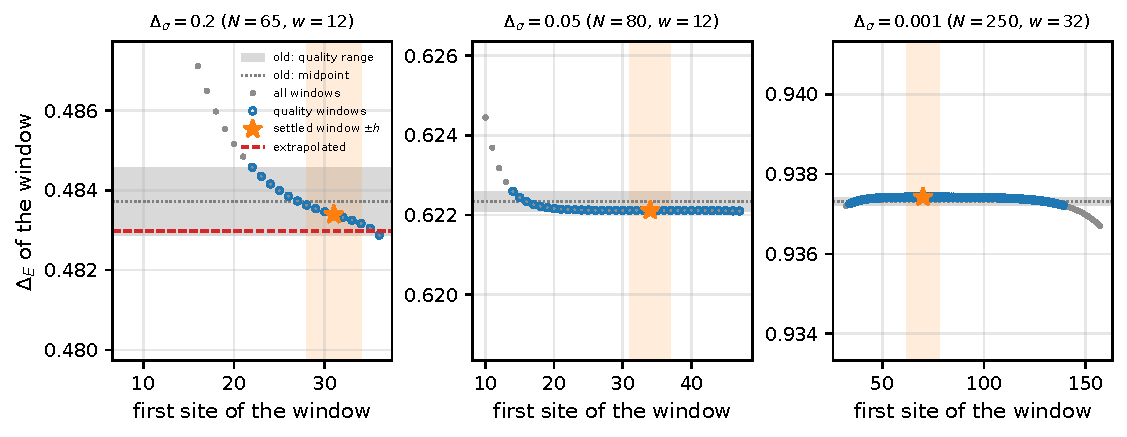
\includegraphics[width=0.98\textwidth]{parts/nrg/figures/fig_plateau.pdf}
\caption{Window audit of three central items: $\DE$ of every window (gray dots) and of the quality windows (open circles) against the
first site of the window; star and orange band: the settled window and its neighborhood $\pm h$; gray band and dotted line: the quality
range and its midpoint, the superseded estimate; dashed (at $\Ds=0.2$): the extrapolated value. The vertical scales differ between
panels. At $\Ds=0.05$ and $0.001$ the quality windows end on a flat plateau, at $0.2$ they drift downward to the end.}\label{nrg:fig:plateau}
\end{figure}

\subsection{The limit \texorpdfstring{$s\to1$}{s -> 1}}\label{nrg:sec:s1}
Table~\ref{nrg:tab:s1} compares $y_t=1-\DE$ with the leading form $\sqrt{2\delta}=2\sqrt{\Ds}$ and the next-to-leading form of
Eq.~\eqref{nrg:eq:s1}. The ratio to the leading form approaches 1 as $s\to1$: $y_t=\nrgytOne$ against $\nrgktOne$ at $\Ds=0.001$
($\nrgktPctOne$\%) and $\nrgytTen$ against $\nrgktTen$ at $0.01$ ($\nrgktPctTen$\%). Against the next-to-leading form $\nrgnloOne$ the
difference at $\Ds=0.001$ is $\nrgnloDiffOne$. The remainder divided by $\delta^{3/2}$ changes smoothly over $0.001\le\Ds\le0.075$
($\nrgnloRatioRange$): it is $\nrgnloRatioTen$ at $\Ds=0.01$, where $\dtot/\delta^{3/2}=\nrgnloRatioErrTen$, and $\nrgnloRatioOne$ at
$0.001$, where $\dtot/\delta^{3/2}=\nrgnloRatioErrOne$ is as large as the entry. The dual expansion~\eqref{nrg:eq:dual} fixes the coefficient
of $\delta^{3/2}$ in $y_t$, $-C^{\rm SR}_3(1)/2^{3/2}=\nrgnloThreeCoef$, which the remainder approaches as $s\to1$.

The accompanying paper~\cite{nrg:Paper} tests the dual expansion directly at $\Ds=0.01$, where $\dtot=\nrgerrTen$. The difference
between $\DE$ and the series~\eqref{nrg:eq:dual} summed through $C^{\rm SR}_n(1)$ is $\nrgsrDiffTwo$, $\nrgsrDiffThree$, $\nrgsrDiffFour$
and $\nrgsrDiffFive$ for $n=2$, 3, 4 and 5: it shrinks to the size of $\dtot$ as $C^{\rm SR}_3(1)$, $C^{\rm SR}_4(1)$ and
$C^{\rm SR}_5(1)$ are added. The term of $C^{\rm SR}_6(1)$, of magnitude $\nrgsrTermSix$, is itself of the size of $\dtot$ and brings
the difference to $\nrgsrDiffSix$; the higher terms lie below $\dtot$. NRG thus reproduces the dual expansion through
$C^{\rm SR}_5(1)$ and is consistent with $C^{\rm SR}_6(1)$.

\begin{table}[ht]\centering\small
\caption{$y_t=1-\DE$ near $s=1$ against the leading form $\sqrt{2\delta}$ ($\delta=1-s=2\Ds$) and the next-to-leading form
$\sqrt{2\delta}-\delta/4$ of Refs.~\cite{nrg:BLMV25,nrg:BLMV26}; the remainder in units of $\delta^{3/2}$, and $\dtot$ in the same units (the
uncertainty of the remainder).}\label{nrg:tab:s1}
\begin{tabular}{@{}llllllrr@{}}
\toprule
$\Delta_\sigma$ & $\delta=1-s$ & $y_t=1-\Delta_E$ & $\sqrt{2\delta}=2\sqrt{\Delta_\sigma}$ & ratio & $\sqrt{2\delta}-\delta/4$ & $(y_t-\sqrt{2\delta}+\delta/4)/\delta^{3/2}$ & $\delta_{\rm tot}/\delta^{3/2}$\\
\midrule
0.075 & 0.15 & 0.43374 & 0.54772 & 0.792 & 0.51022 & -1.32 & 0.00051\\
0.05 & 0.1 & 0.37788 & 0.44721 & 0.845 & 0.42221 & -1.40 & 0.00085\\
0.025 & 0.05 & 0.28658 & 0.31623 & 0.906 & 0.30373 & -1.53 & 0.0026\\
0.01 & 0.02 & 0.19025 & 0.20000 & 0.951 & 0.19500 & -1.68 & 0.017\\
0.001 & 0.002 & 0.06258 & 0.06325 & 0.989 & 0.06275 & -1.90 & 1.2\\
\bottomrule
\end{tabular}

\end{table}

% =====================================================================================================================
\section{Checks}\label{nrg:sec:checks}
% =====================================================================================================================
A second implementation of the same numerical map tests the code (Sec.~\ref{nrg:sec:indep}); two methods that do not use NRG test the
method (Secs.~\ref{nrg:sec:series} and~\ref{nrg:sec:mc}); Sec.~\ref{nrg:sec:literature} lists published values. Figure~\ref{nrg:fig:checks} summarizes
the comparisons.

\subsection{A second implementation}\label{nrg:sec:indep}
\paragraph{Design.} Claude Code, which knew the production code, wrote a specification of the physics and conventions only
(\code{independent\_check/SPEC.md}). It fixed the discretization, the chain, the truncation per parity sector, the critical-search rule
and the window rule, and forbade access to the production code, data and this note. From it a separate Claude agent wrote a second
solver (\code{independent\_check/indep\_nrg.py}); that it did not open the forbidden files rests on the instruction and on the agent's
own statement in \code{NOTES.md}, not on an access log. Every algorithmic choice differs from production:
\begin{center}\footnotesize
\begin{tabular}{@{}p{2.6cm}p{5.4cm}p{7.6cm}@{}}\toprule
 & production (\code{lri\_spin}) & second implementation (\code{indep\_nrg.py})\\\midrule
chain coefficients & closed form~\eqref{nrg:eq:coeff} & Lanczos with full reorthogonalization on the star, in mpmath\\
parity blocks & basis order of the reference solver & NumPy Kronecker order, generic operators\\
eigensolver & partial spectrum (flows), full (derivative) & full spectrum everywhere\\
$y_t$ & exact derivative~\eqref{nrg:eq:tangent} & central finite differences in $\alpha$, relative steps $\eta=10^{-9},10^{-10},10^{-11}$\\
window audit & package code & written from the specification\\\bottomrule
\end{tabular}
\end{center}
The Lanczos recursion runs with $40+1.3N\log_{10}\Lambda$ decimal digits and is repeated with 40 more digits and 40 more star modes to
check convergence. The second implementation has its own 38 self-tests (for example, the chain reproduces the star to $3\times10^{-50}$,
and the NRG reproduces exact diagonalization of untruncated systems to $5\times10^{-15}$). Eight configurations c1--c8 with
$0.502\le s\le0.998$, $\Lambda=2$, $2.5$ and $3$, $K=48$ or $64$ and $n_b=10$--$16$ ran on one cluster node, one single-core process
each, the longest in $\nrgindWall$\,min; each is compared with the production record of the same item.

\paragraph{Result.} Table~\ref{nrg:tab:indep} lists the comparison.
\begin{itemize}
\item The chain coefficients agree to better than $\nrgindChain$ (relative): to rounding, whose last bits depend on the platform. The
  closed form is confirmed.
\item The critical couplings are bitwise identical in $\nrgindAlphaBitwise$ configurations and agree to $\nrgindAlpha$ in the others.
  The critical flows agree to $\nrgindFlow$ over the first eleven sites.
\item A window's finite-difference $\DE$ is \emph{trusted} when two neighboring steps $\eta$ agree to $10^{-6}$. In all
  $\nrgindTrusted$ trusted windows ($\nrgindTrustedMin$ to $\nrgindTrustedMax$ per configuration) the two implementations agree to
  $\nrgindDE$, with median $\nrgindDEmedian$, far below the quoted errors. In the $\nrgindSettledN$ configurations whose settled window
  is trusted, they agree there to $\nrgindSettled$.
\item The latest windows of a chain lie beyond the reach of finite differences, because $\eta\,\alpha\,\Lambda^{y_tn}$ is no longer
  small there. Only $\nrgindCovered$ of the $\nrgindQuality$ production quality windows are within reach. All quality windows of a
  configuration are within reach only in $\nrgindFullList$; at $s=0.502$ (c5) none is. This is a limit of the check, not a
  disagreement.
\end{itemize}
The check verifies the numerical map at $K\le64$. It does not test the central items at $K=128$, $n_b=16$ directly (they differ only in
$K$ and $n_b$), the estimator (it shares the window rule by construction), or the limit $\Lambda\to1$. Both implementations come from
the same model family, and the specification was written by the agent that knew the production code: the check tests the code, not
shared conceptual choices.

\begin{table}[ht]\centering\scriptsize\setlength{\tabcolsep}{4pt}
\caption{Second implementation against production. Columns: configuration $(s,\Lambda,K,n_b,N)$; largest relative difference of the
rescaled chain coefficients (a rounding-level bound); relative difference of $\alpha_c$; number of trusted windows; largest window-by-window difference
$|\delta\DE|$ over them; production quality windows within finite-difference reach (covered/all); production quality range.}\label{nrg:tab:indep}
\begin{tabular}{@{}lllllrrl@{}}
\toprule
id & $(s,\Lambda,K,n_b,N)$ & chain & $\alpha_c$ & trusted & $\max|\delta\Delta_E|$ & covered & quality range (production)\\
\midrule
c1 & $(0.8,3,64,10,65)$ & $<10^{-15}$ & bitwise & 19 & $2\times10^{-7}$ & 13/23 & [0.529612, 0.530062]\\
c2 & $(0.9,3,64,10,80)$ & $<10^{-15}$ & $4\times10^{-14}$ & 27 & $9\times10^{-8}$ & 23/34 & [0.622119, 0.622597]\\
c3 & $(0.98,3,64,10,105)$ & $<10^{-15}$ & bitwise & 53 & $3\times10^{-7}$ & 41/41 & [0.809460, 0.810127]\\
c4 & $(0.6,3,64,12,65)$ & $<10^{-15}$ & bitwise & 17 & $2\times10^{-7}$ & 3/15 & [0.483316, 0.484567]\\
c5 & $(0.502,3,64,16,65)$ & $<10^{-15}$ & bitwise & 18 & $2\times10^{-7}$ & 0/2 & [0.508000, 0.508268]\\
c6 & $(0.998,3,48,10,250)$ & $<10^{-15}$ & $4\times10^{-14}$ & 126 & $2\times10^{-7}$ & 106/106 & [0.937223, 0.937429]\\
c7 & $(0.8,2,64,10,103)$ & $<10^{-15}$ & $7\times10^{-14}$ & 34 & $2\times10^{-7}$ & 28/46 & [0.529796, 0.531050]\\
c8 & $(0.7,2.5,64,10,78)$ & $<10^{-15}$ & bitwise & 22 & $2\times10^{-7}$ & 14/29 & [0.491178, 0.492328]\\
\bottomrule
\end{tabular}

\end{table}

\subsection{The \texorpdfstring{$\varepsilon$}{epsilon} expansion near \texorpdfstring{$s=1/2$}{s = 1/2}}\label{nrg:sec:series}
\paragraph{Reference.} The accompanying paper gives $\De=\sum_{n=0}^{8}C_n\varepsilon^n$ for $d=1$~\cite{nrg:Paper}, with
$C_0=1/2$, $C_1=-1/6$, $C_2=0.657131263981$, $C_3=-3.719856322902$, $C_4=45.42488010356$, $C_5=-731.13947662454$ and
$C_6=14331.6870328$ (exact to the digits shown), $C_7=-322550\pm40$ and $C_8=(8.060\pm0.017)\times10^6$. The uncertainties of $C_7$
and $C_8$ are the paper's allowances, mostly four sampling standard errors. They are not part of the Borel--Pad\'e spread below;
shifting $C_7$ or $C_8$ by about its allowance moves the $[4/4]$ approximant by at most $\nrgserSensTwoTwentyFive$ at $\Ds=0.225$ and
$\nrgserSensTwoHundred$ at $0.2$, less than the spread at both points. The coefficients grow factorially, so the series is asymptotic.
We evaluate it in two ways (\code{method\_comparison/compare\_methods.py}):
\begin{itemize}
\item \textbf{optimal truncation}: the partial sum up to, but excluding, the smallest term, with that term as its error;
\item \textbf{Borel--Pad\'e}: Pad\'e approximants $[L/M]$ of the Borel transform $\sum_nC_nu^n/n!$ with $L+M=6,7,8$, keeping those
  without a pole on the positive axis and with a value between 0.3 and 1.2, Laplace-transformed back. The central value is the upper
  of the two middle values of the $L+M=8$ approximants (there are four at $0.2\le\Ds\le0.24$), not their mean; the error is the
  half-range of all approximants with $L+M\ge7$. The $L+M=6$ approximants are computed but enter neither. The choice of the upper
  middle value is a convention of the comparison script of 8 October 2026, unchanged since and not chosen with the present NRG values
  in view; it has no further justification. At $\Ds\ge0.225$, where the approximants agree to within the quoted spread, it hardly
  matters; at $\Ds=0.2$ it does (below).
\end{itemize}
The reference is the partial sum at $\Ds=0.249$ ($\varepsilon=0.004$), where all terms decrease and the error is
$\nrgserOptErrTwoFortyNine$ (Borel--Pad\'e gives $\nrgserBpTwoFortyNine$ too), and the Borel--Pad\'e sum at larger $\varepsilon$. At
$\Ds=0.24$ the two evaluations agree to $\nrgserAgreeTwoForty$. At $0.225$ the Borel--Pad\'e sum, $\nrgserTwoTwentyFive$, has a small
spread, but optimal truncation gives $\nrgserOptTwoTwentyFive$, so the reference there depends on the resummation. At $\Ds=0.2$ the
spread, $\nrgserSpreadTwoHundred$, is too large to test NRG at the $10^{-3}$ level.

\paragraph{Result.} Table~\ref{nrg:tab:series}. At $\Ds=0.2$ the series does not test NRG: the extrapolated NRG value lies
$\nrgdiffTwoHundred$ from the central approximant, a coincidence of the convention above, and $\nrgdiffMedTwoHundred$ from the median
$\nrgbpMedTwoHundred$ of the $\nrgbpNTwoHundred$ approximants with $L+M=8$, which range from $\nrgbpLoTwoHundred$ to
$\nrgbpHiTwoHundred$; both differences are well inside the spread, and neither is evidence for or against NRG. At the three points not converged in chain depth the settled values lie above the series by $\nrgexcTwoFortyNine$,
$\nrgexcTwoForty$ and $\nrgexcTwoTwentyFive$, decreasing with $\varepsilon$, as the slow approach of Sec.~\ref{nrg:sec:approach} predicts.
Two extrapolations serve as cross-checks; neither is adopted:
\begin{itemize}
\item \textbf{The rule's own extrapolation} (Sec.~\ref{nrg:sec:estimator}) is not stable there. Over the three fit ranges and
  $\Lambda=2.5$, $3$ it gives $\nrgextLoTwoForty$--$\nrgextHiTwoForty$ ($\nrgextExcLoTwoForty$ to $\nrgextExcHiTwoForty$ from the series)
  at $\Ds=0.24$, and $\nrgextLoTwoTwentyFive$--$\nrgextHiTwoTwentyFive$ ($\nrgextExcLoTwoTwentyFive$ to $\nrgextExcHiTwoTwentyFive$) at
  $0.225$. At $\Ds=0.249$, where $\varepsilon l_{\max}\approx0.25$, a single exponential cannot represent the $1/l$ approach, and the
  extrapolation ($\nrgextLoTwoFortyNine$--$\nrgextHiTwoFortyNine$) removes less than half of the excess.
\item \textbf{The crossover fit} of Sec.~\ref{nrg:sec:crosscheck} is stable and moves the values toward the series, but not onto it. At
  $\Ds=0.225$ it gives $\nrgcrossTwoTwentyFive$ ($\nrgcrossNTwoTwentyFive$ accepted fits, $\nrgcrossLoTwoTwentyFive$ to
  $\nrgcrossHiTwoTwentyFive$, i.e.\ $\nrgcrossExcLoTwoTwentyFive$ to $\nrgcrossExcHiTwoTwentyFive$ from the series value
  $\nrgserTwoTwentyFive$). At $0.24$ it gives $\nrgcrossTwoForty$ ($\nrgcrossLoTwoForty$ to $\nrgcrossHiTwoForty$): every accepted fit
  lies above the series value $\nrgserTwoForty$, by $\nrgcrossExcLoTwoForty$ to $\nrgcrossExcHiTwoForty$, against $\nrgexcTwoForty$ for
  the settled value. At $0.249$ it gives $\nrgcrossTwoFortyNine$, $\nrgcrossExcTwoFortyNine$ from the series: there the fit is
  ill-conditioned, and the one-loop test of Sec.~\ref{nrg:sec:approach} is the relevant check.
\end{itemize}

\paragraph{Interpretation.} The excess is the expected crossover from the strong bare coupling of the spin--boson model to the
interacting fixed point, whose correction exponent $\omega\approx\varepsilon$ vanishes at $s=1/2$; within $l_{\max}$ the flow has not
arrived. It depends only on the RG time, not on $K$, $n_b$ or $\Lambda$ at fixed depth (Sec.~\ref{nrg:sec:approach}), and at
$\Ds=0.249$ it decays at a rate of the one-loop size. Logarithmic corrections of this kind were already seen in NRG at $s=1/2$~\cite{nrg:Vojta2005}.
An earlier version of this note attributed the excess to the known truncation errors of bosonic NRG near Gaussian fixed points
(Hilbert-space truncation and mass flow~\cite{nrg:Vojta2005,nrg:Vojta2010,nrg:Vojta2012}). The data do not support that: those errors affect
order-parameter exponents below $s=1/2$, and for $s>1/2$ the mass-flow correction changes the flows only quantitatively
(at $s=0.6$, ``no qualitative difference between the flows without and with mass-flow correction''~\cite{nrg:Vojta2010}); we have no run
that isolates either effect. The same mechanism acts at $\Ds=0.2$ and $0.175$ at a smaller level (shifts $\nrgextShiftTwoHundred$ and
$\nrgextShiftOneSeventyFive$ from settled to extrapolated), where the extrapolation is stable and its full length is in $\dd$.

\paragraph{Decision.} The three values at $\Ds=0.249$, $0.24$ and $0.225$ are kept as computed (the settled values), marked ``not
converged in chain depth'', shown in the tables and figures, and used in no comparison and no agreement statement. This is the
author's decision. The label is not an outcome of the estimator, and it was assigned when this comparison was already known
(Sec.~\ref{nrg:sec:estimator}); App.~\ref{nrg:app:provenance} gives its history, including an earlier recommendation that the author
overruled.

\begin{table}[ht]\centering\scriptsize\setlength{\tabcolsep}{3pt}
\caption{NRG against the $\varepsilon$ series near $s=1/2$. Optimal truncation with its smallest term; Borel--Pad\'e central value with
the spread over approximants; NRG minus the reference (the partial sum at $\Ds=0.249$, the Borel--Pad\'e sum otherwise; at $\Ds=0.2$
this difference is not meaningful, see text); the range of the rule's extrapolations and the crossover fit of
Sec.~\ref{nrg:sec:crosscheck} (cross-checks, not adopted). Bracketed: settled values not converged in chain depth, not used.}\label{nrg:tab:series}
\begin{tabular}{@{}llllllll@{}}
\toprule
$\Delta_\sigma$ & $\varepsilon$ & NRG $\Delta_E$ & optimal truncation & Borel--Pad\'e (spread) & NRG $-$ reference & rule's extrapolation & crossover fit\\
\midrule
0.249 & 0.004 & [0.508030] & 0.499344 ($\pm5\times10^{-13}$) & 0.49934 ($6\times10^{-15}$) & $+8.7\times10^{-3}$ & 0.5046--0.5057 & 0.50209\\
0.24 & 0.04 & [0.498922] & 0.494194 ($\pm5\times10^{-5}$) & 0.49422 ($2\times10^{-7}$) & $+4.7\times10^{-3}$ & 0.4934--0.4970 & 0.49460\\
0.225 & 0.1 & [0.489668] & 0.489905 ($\pm4\times10^{-3}$) & 0.48808 ($1\times10^{-4}$) & $+1.6\times10^{-3}$ & 0.4867--0.4888 & 0.48810\\
0.2 & 0.2 & 0.4830(7) & 0.466667 ($\pm0.03$) & 0.48292 ($9\times10^{-3}$) & $+5.9\times10^{-5}$ & adopted & 0.48305\\
\bottomrule
\end{tabular}

\end{table}

\subsection{The 1D cluster Monte Carlo study}\label{nrg:sec:mc}
\paragraph{Reference.} The Monte Carlo study of the same model in this repository (\code{MC/} folder~\cite{nrg:MCnote}; Fukui--Todo
cluster algorithm~\cite{nrg:FukuiTodo2009,nrg:LB95} with finite-size scaling) is the project's own, run by the same AI systems; it is
independent of NRG in method, not in authorship. We use only its quoted values and labels; their definitions are in its
note~\cite{nrg:MCnote}. In brief, its value of $\De$ comes from a finite-size-scaling fit of all lattice sizes, with a statistical error
$\sigma_{\rm stat}$ and a systematic scale $\sigma_{\rm sys}$, the half-range of the values over a family of fit models (a sensitivity
scale, not a standard deviation). As a cross-check it also extrapolates in the lattice size the crossings, between pairs of sizes, of a
finite-size-scaling observable; this \emph{crossing extrapolation} is quoted as $\De^\infty(\sigma_\infty)(\Delta_{\omega'})$, with
error $\sigma_\infty$ and sensitivity $\Delta_{\omega'}$ to the assumed correction exponent $\omega'$ ($\Delta_{\omega'}$ is a
sensitivity, not a dimension). Each value carries a label: \textbf{accepted}, the fit value and the crossing extrapolation agree within
twice the error of their difference (``$\sigma_{\rm sys}$-dominated'' marks values whose $\sigma_{\rm sys}$ is much larger than
$\sigma_{\rm stat}$); \textbf{cross-check failed}, they differ by more, and the study does not certify the value as an infinite-size
value; \textbf{cross-check unavailable}, fewer than two size series are available for the crossing extrapolation; \textbf{conditional},
$\sigma_{\rm sys}$ could not be estimated.

\paragraph{Result.} Table~\ref{nrg:tab:mc}.
\begin{itemize}
\item \textbf{Accepted ($\Ds=\nrgmcAccList$).} NRG and Monte Carlo differ by at most $\nrgmcAccDiffMax$ (at $\Ds=\nrgmcAccDiffMaxAt$).
  The differences exceed the Monte Carlo statistical errors, by up to $\nrgmcAccStatRatioMax\,\sigma_{\rm stat}$, and have the same
  sign at neighboring points (below). They lie within $\sigma_{\rm sys}$ at $\nrgmcAccWithinSys$ of the $\nrgmcAccN$ points and within
  $\sigma_{\rm stat}+\sigma_{\rm sys}+\dtot$ at $\nrgmcAccWithinLin$, the largest ratio being $\nrgmcAccRatioMax$ at
  $\Ds=\nrgmcAccDiffMaxAt$. This linear sum adds a standard deviation, a fit-model half-range and an NRG error scale; we use it as a
  scale for the size of the differences, not as a test of statistical consistency. At $\Ds=\nrgmcAccDiffMaxAt$ the Monte Carlo
  crossing extrapolation agrees with NRG to $\nrgmcCrossOneHundred\,\sigma_\infty$; at all $\nrgmcAccN$ accepted points it agrees
  within $\nrgmcCrossStatMax\,\sigma_\infty$, and within $\nrgmcCrossRatioMax$ of $\sigma_\infty+\Delta_{\omega'}+\dtot$. The NRG
  errors are smaller than $\sigma_{\rm sys}$ by factors $\nrgmcAccSysRatio$, so the comparison tests the Monte Carlo systematics more
  than it tests NRG; only $\sigma_{\rm sys}$ reconciles the two.
\item \textbf{Cross-check failed ($\Ds=\nrgmcCcfList$).} These are not infinite-size values, and we use them only to say where NRG lies:
  at $0.175$ between the fit and the crossing extrapolation ($\nrgmcFitOneSeventyFive$ from the fit, $\nrgmcCrossOneSeventyFive$ from
  the crossing), at $0.15$ below both ($\nrgmcFitOneFifty$ and $\nrgmcCrossOneFifty$). Including these two points, the crossing
  extrapolations agree with NRG within $\nrgmcCrossAllMax\,\sigma_\infty$ at all $\nrgmcCrossAllN$ common points.
\item \textbf{Correlated signs.} NRG lies below the Monte Carlo fit at $\nrgmcNeg$ consecutive points of the $\nrgmcBoth$
  ($0.175$ to $0.075$) and above it at $0.05$ and $0.025$. The differences are therefore not independent fluctuations; they look like
  a smooth systematic of one of the two methods, which the Monte Carlo $\sigma_{\rm sys}$ is meant to cover.
\item \textbf{$\Ds=0.225$} is conditional in the Monte Carlo study and not converged in NRG; the Monte Carlo value lies
  $\nrgmcTwoTwentyFiveSer$ from the series. It enters no comparison.
\end{itemize}

\begin{table}[ht]\centering\scriptsize\setlength{\tabcolsep}{3.5pt}
\caption{NRG against the 1D cluster Monte Carlo study at the common points. MC value with $\sigma_{\rm stat}$ and $\sigma_{\rm sys}$ in
units of the last digit, and its label (Sec.~\ref{nrg:sec:mc}); NRG minus MC; ``ratio'' is $|{\rm NRG}-{\rm MC}|$ divided by
$\sigma_{\rm stat}+\sigma_{\rm sys}+\dtot$ (shown also for the cross-check-failed points, which are not infinite-size values); MC
crossing extrapolation with $\sigma_\infty$ and $\Delta_{\omega'}$. MC values are quoted as that study gives them. $^\ast$Not
converged in NRG, not used.}\label{nrg:tab:mc}
\begin{tabular}{@{}lllllll@{}}
\toprule
$\Delta_\sigma$ & NRG $\Delta_E$ & MC $\Delta_\varepsilon$ ($\sigma_{\rm stat}$)($\sigma_{\rm sys}$) & MC label & NRG $-$ MC & ratio & MC crossing ($\sigma_\infty$)($\Delta_{\omega^\prime}$)\\
\midrule
0.225$^\ast$ & [0.4897] & 0.47912(68)(--) & conditional (no $\sigma_{\rm sys}$) & $+0.011$ & -- & --\\
0.175 & 0.48390(35) & 0.48460(35)(67) & cross-check failed & $-7.0\times10^{-4}$ & 0.51 & 0.48304(81)(1)\\
0.15 & 0.49111(11) & 0.49325(41)(306) & cross-check failed & $-2.1\times10^{-3}$ & 0.60 & 0.49183(71)(70)\\
0.125 & 0.50567(5) & 0.50710(35)(193) & accepted & $-1.4\times10^{-3}$ & 0.61 & 0.50640(172)(392)\\
0.1 & 0.529608(33) & 0.53248(20)(242) & accepted ($\sigma_{\rm sys}$-dom.) & $-2.9\times10^{-3}$ & 1.08 & 0.52975(135)(248)\\
0.075 & 0.566260(30) & 0.56694(37)(139) & accepted & $-6.8\times10^{-4}$ & 0.38 & 0.56843(207)(1044)\\
0.05 & 0.622115(27) & 0.61987(55)(220) & accepted & $+2.2\times10^{-3}$ & 0.81 & 0.62393(348)(773)\\
0.025 & 0.713422(29) & 0.71115(49)(959) & accepted ($\sigma_{\rm sys}$-dom.) & $+2.3\times10^{-3}$ & 0.22 & 0.70906(902)(1509)\\
\bottomrule
\end{tabular}

\end{table}

\subsection{Published values}\label{nrg:sec:literature}
\begin{itemize}
\item \textbf{1D LRI Monte Carlo.} Uzelac, Glumac and Ani\v{c}i\'c~\cite{nrg:UGA01} give $1/\nu=0.50(2)$, $0.51(2)$, $0.47(2)$ and $0.40(1)$ at
  $s=0.6$, $0.7$, $0.8$ and $0.9$, i.e.\ $\De=0.50(2)$, $0.49(2)$, $0.53(2)$ and $0.60(1)$ at $\Ds=0.2$, $0.15$, $0.1$ and $0.05$. NRG
  differs from them by $\nrgugaTwoHundred$, $\nrgugaOneFifty$, $\nrgugaOneHundred$ and $\nrgugaFifty$ of their errors; at $\Ds=0.05$ the
  project's Monte Carlo value, $0.61987(55)(220)$, also lies above theirs. Angelini, Parisi and Ricci-Tersenghi~\cite{nrg:APR14} give
  $1/\nu=0.4124(13)$ at $s=0.875$ ($\De=0.5876(13)$ at $\Ds=0.0625$) and $0.506(14)$ at $s=0.65453$; neither point is on our grid.
  Four interpolations of our final values (a cubic spline over $0.01\le\Ds\le0.15$ and polynomials through three or four neighboring
  points) give $\nrgaprLo$--$\nrgaprHi$ at $\Ds=0.0625$, $\nrgaprSigLo$ to $\nrgaprSigHi$ of their errors above $0.5876$; the project's
  Monte Carlo study gives $0.59003(35)(150)$ there (label: cross-check unavailable).
\item \textbf{The spin--boson model.} Bosonic NRG~\cite{nrg:Bulla2003,nrg:Vojta2005} and continuous-time quantum Monte
  Carlo~\cite{nrg:WRVB09} give $1/\nu$ (or $\nu z$) for $s>1/2$ only in figures. Read off the figures by eye, the NRG values of
  Ref.~\cite{nrg:Vojta2005} are about $0.50$, $0.50$, $0.46$, $0.37$ and $0.28$ at $s=0.6$, $0.7$, $0.8$, $0.9$ and $0.95$, against our
  $y_t=\nrgytFig$, and the quantum Monte Carlo values agree with both within their error bars; this is
  agreement at the resolution of the figures, a few hundredths, not a quantitative test. Other methods for this
  model~\cite{nrg:AF09,nrg:Guo2012} report order-parameter exponents, not $\nu$.
\item \textbf{Functional RG and the hierarchical model}~\cite{nrg:PGTD26} give $1/\nu$ for $1/2<s<1$ in figures; near $s=1$ they quote
  the form of Eq.~\eqref{nrg:eq:s1}.
\end{itemize}

% =====================================================================================================================
\section{Limitations and open problems}\label{nrg:sec:limits}
% =====================================================================================================================
\begin{enumerate}
\item \textbf{Chain depth near $s=1/2$.} At $\Ds=0.249$, $0.24$ and $0.225$ the flow does not reach its fixed point within the RG time
  that double precision allows (Sec.~\ref{nrg:sec:approach}). The crossover fit of Sec.~\ref{nrg:sec:crosscheck} (cross-check, not adopted) is
  stable there and gives $\nrgcrossTwoTwentyFive$ and $\nrgcrossTwoForty$ at $\Ds=0.225$ and $0.24$, closer to the series than the
  settled values but above it at $0.24$; it is ill-conditioned at $0.249$ (Sec.~\ref{nrg:sec:series}). Extended precision (longer
  $l_{\max}$) would remove the need to extrapolate. At $\Ds=0.2$ and $0.175$ the values are extrapolations; they depend on the fit
  form, and $\dd$ covers the full extrapolation length.
\item \textbf{Continuum limit.} Over $2\le\Lambda\le4$ the plateau values change by at most a few $10^{-5}$, monotonically, but
  $\Lambda<2$ is not reached, $K$ convergence at $\Lambda=2.5$ rests on one doubling (covered by an allowance) and at $\Lambda=4$ is
  assumed. At $\Ds=0.001$ the plateau depends on $K$ at $\Lambda\neq3$ at the $10^{-4}$ level. Runs at $\Lambda\le1.5$ with more than
  128 kept states, or at $\Lambda=2$ with $K\ge192$ at all points, would improve this. At $K=512$ and $n_b=10$ a parity block has
  dimension about 5000, which dense diagonalization handles, but it must be repeated at every site of every bisection step.
\item \textbf{Universality in $\Omega$.} All runs use $\Omega=0.1$. A second $\Omega$ at one or two points would test universality and
  the reading of the approach as a correction to scaling (the $l$ dependence should move, the plateau value not).
\item \textbf{Error model.} The errors are scales, not standard deviations; the linear sum, the plateau threshold, the fit form and
  ranges, the full extrapolation length and the $K$-doubling allowance are judgements (Sec.~\ref{nrg:sec:budget}). The estimator was
  chosen after the NRG data and after an earlier comparison had been seen, and the label ``not converged in chain depth'' was assigned
  after the comparison with the $\varepsilon$ series.
\item \textbf{Coverage of the second implementation.} It ran at $K\le64$, could not reach the latest windows, including both quality
  windows at $s=0.502$, and shares the window rule (Sec.~\ref{nrg:sec:indep}).
\item \textbf{Review.} The analysis, the estimator and this note were reviewed only by AI agents: two rounds on 13 October 2026 by
  agents of the same family as the AI that wrote them, and a reading on 15 October (App.~\ref{nrg:app:provenance}). The changes made after
  the second round and after the reading have not been reviewed again.
\item \textbf{Not needed.} Hamiltonian-truncation calculations of the same model~\cite{nrg:Paper,nrg:HTnote} need a correction for a fixed energy cutoff on a free
  Fock space. NRG truncates iteratively in the interacting basis, keeps the complete new site for every kept state and is
  non-perturbative in $\alpha$, so no such correction applies, and none was added.
\end{enumerate}

% =====================================================================================================================
\section{Reproduction}\label{nrg:sec:repro}
% =====================================================================================================================
\subsection{The released folder}
The \code{NRG/} folder of the repository contains:
\begingroup\raggedright
\begin{itemize}
\item \code{code/lri\_spin\_boson\_hpc/}: the solver, its tests, the reference solver of the original study and the cluster tools
  (App.~\ref{nrg:app:provenance} lists what was removed from the original tree);
\item \code{code/campaigns/}: the generators of the item lists in \code{inputs/items/};
\item \code{code/analysis/}: the analysis stages (\code{summarize.py}, \code{estimator.py},
  \code{build\_tables.py}, \code{make\_figures.py}, \code{note\_numbers.py}, \code{check\_figures.py}) and the
  collector of cluster records, \code{collect\_records.py};
\item \code{inputs/}: the item lists, the frozen manifests that were submitted, the validation receipt and the environment record;
\item \code{data/}: the $\nrgnItems$ result records, the per-job lane logs and the job accounting;
\item \code{results/}: the final table (\code{ds13\_final.json}, \code{ds13\_final\_table.md}) and the $\Lambda$ study;
\item \code{independent\_check/}, \code{independent\_check\_compare/}, \code{method\_comparison/}: the checks of Sec.~\ref{nrg:sec:checks};
\item \code{verify/}: the verifier, the expected values and the smoke-test reference; \code{slurm/}: job templates; \code{note/}: this
  note.
\end{itemize}
\endgroup
\noindent\code{README.md}, \code{REPRODUCE.md}, \code{PROVENANCE.md}, \code{REVIEWS.md} and \code{data/DATA.md} in that folder give the details.

\subsection{How to run}
From \code{NRG/}, with Python $\ge3.10$, NumPy, SciPy, threadpoolctl, mpmath, matplotlib and pytest:
\begin{itemize}
\item \code{make test} (about 75\,s on one core of a recent laptop): the 85 solver tests, the checksum list of the code, and the 38
  self-tests of the second implementation.
\item \code{make replay} (20--30\,s): checks the solver source hash, verifies every record (checksum, identity against its manifest and
  the receipt, numerical gates), recomputes all results, tables, in-text numbers and figures of this note in a hidden workspace
  \code{.work/}, and compares them with the released files and with \code{verify/expected.json}. It also needs the Monte Carlo table of
  the repository, \code{../MC/data/1d/scan\_data/FIT\_V3\_SCAN.json} (\code{make replay MCSCAN=<path>} to point elsewhere). The
  extrapolations are least-squares fits whose last bits depend on the NumPy/SciPy build and the CPU, so the comparison uses
  tolerances (about $10^{-9}$ for values, one unit of the last printed digit for tables), not byte identity (\code{REPRODUCE.md}).
\item \code{make smoke} (about 15\,s): one small critical search with both solvers, compared with each other and with the
  reference values in \code{verify/smoke\_expected.json}.
\item \code{make note}: rebuilds this note in place from the released tables and figures.
\end{itemize}
Rerunning production needs a Slurm cluster: $\nrgthreadHours$ thread-hours, about $\nrgnodeHours$ node-hours of whole-node allocations
(\code{REPRODUCE.md}). On another runtime the exponents are expected to agree within the quoted errors, while $\alpha_c$ moves at the
$10^{-13}$ level and late flows at fixed $\alpha$ differ (Sec.~\ref{nrg:sec:software}); no full rerun on a second runtime was made.

% =====================================================================================================================
\begin{thebibliography}{99}
\bibitem{nrg:Paper} The accompanying paper on the long-range Ising model (in preparation): $\varepsilon$-expansion coefficients
  $C_0,\dots,C_8$ for $d=1$, with their derivations in the \code{GFF/} folder of this repository.
\bibitem{nrg:MCnote} \emph{Monte Carlo determination of the thermal dimension $\De(\Ds)$ of the long-range Ising model in $d=1,2,3$},
  note in the \code{MC/} folder of this repository (2026).
\bibitem{nrg:HTnote} Notes on Hamiltonian truncation of the long-range Ising model, in the \code{HT/} folder of this repository (2026).
\bibitem{nrg:Fisher1972} M.~E.~Fisher, S.-k.~Ma, and B.~G.~Nickel, \emph{Critical exponents for long-range interactions}, Phys.\ Rev.\
  Lett.\ \textbf{29}, 917 (1972).
\bibitem{nrg:Sak1973} J.~Sak, \emph{Recursion relations and fixed points for ferromagnets with long-range interactions}, Phys.\ Rev.\ B
  \textbf{8}, 281 (1973).
\bibitem{nrg:Kosterlitz1976} J.~M.~Kosterlitz, \emph{Phase transitions in long-range ferromagnetic chains}, Phys.\ Rev.\ Lett.\
  \textbf{37}, 1577 (1976).
\bibitem{nrg:LM01} E.~Luijten and H.~Me\ss{}ingfeld, \emph{Criticality in one dimension with inverse square-law potentials}, Phys.\ Rev.\
  Lett.\ \textbf{86}, 5305 (2001), arXiv:cond-mat/0104175.
\bibitem{nrg:BLMV25} D.~Benedetti, E.~Lauria, D.~Maz\'a\v{c}, and P.~van Vliet, \emph{One-dimensional Ising model with $1/r^{1.99}$
  interaction}, Phys.\ Rev.\ Lett.\ \textbf{134}, 201602 (2025), arXiv:2412.12243.
\bibitem{nrg:BLMV26} D.~Benedetti, E.~Lauria, D.~Maz\'a\v{c}, and P.~van Vliet, \emph{A strong-weak duality for the 1d long-range Ising
  model}, SciPost Phys.\ \textbf{20}, 029 (2026), arXiv:2509.05250.
\bibitem{nrg:Leggett1987} A.~J.~Leggett, S.~Chakravarty, A.~T.~Dorsey, M.~P.~A.~Fisher, A.~Garg, and W.~Zwerger, \emph{Dynamics of the
  dissipative two-state system}, Rev.\ Mod.\ Phys.\ \textbf{59}, 1 (1987).
\bibitem{nrg:Wilson1975} K.~G.~Wilson, \emph{The renormalization group: Critical phenomena and the Kondo problem}, Rev.\ Mod.\ Phys.\
  \textbf{47}, 773 (1975).
\bibitem{nrg:Bulla2003} R.~Bulla, N.-H.~Tong, and M.~Vojta, \emph{Numerical renormalization group for bosonic systems and application to
  the sub-Ohmic spin-boson model}, Phys.\ Rev.\ Lett.\ \textbf{91}, 170601 (2003), arXiv:cond-mat/0306708.
\bibitem{nrg:Bulla2005} R.~Bulla, H.-J.~Lee, N.-H.~Tong, and M.~Vojta, \emph{Numerical renormalization group for quantum impurities in a
  bosonic bath}, Phys.\ Rev.\ B \textbf{71}, 045122 (2005), arXiv:cond-mat/0407559.
\bibitem{nrg:Bulla2008} R.~Bulla, T.~A.~Costi, and T.~Pruschke, \emph{Numerical renormalization group method for quantum impurity
  systems}, Rev.\ Mod.\ Phys.\ \textbf{80}, 395 (2008).
\bibitem{nrg:Vojta2005} M.~Vojta, N.-H.~Tong, and R.~Bulla, \emph{Quantum phase transitions in the sub-Ohmic spin-boson model: Failure of
  the quantum-classical mapping}, Phys.\ Rev.\ Lett.\ \textbf{94}, 070604 (2005); Erratum: Phys.\ Rev.\ Lett.\ \textbf{102}, 249904
  (2009), arXiv:cond-mat/0410132.
\bibitem{nrg:Vojta2006} M.~Vojta, \emph{Impurity quantum phase transitions}, Philos.\ Mag.\ \textbf{86}, 1807 (2006).
\bibitem{nrg:Vojta2010} M.~Vojta, R.~Bulla, F.~G\"uttge, and F.~Anders, \emph{Mass-flow error in the numerical renormalization-group
  method and the critical behavior of the sub-Ohmic spin-boson model}, Phys.\ Rev.\ B \textbf{81}, 075122 (2010), arXiv:0911.4490.
\bibitem{nrg:Vojta2012} M.~Vojta, \emph{Numerical renormalization group for the sub-Ohmic spin-boson model: A conspiracy of errors},
  Phys.\ Rev.\ B \textbf{85}, 115113 (2012), arXiv:1201.4922.
\bibitem{nrg:Guo2012} C.~Guo, A.~Weichselbaum, J.~von Delft, and M.~Vojta, \emph{Critical and strong-coupling phases in one- and two-bath
  spin-boson models}, Phys.\ Rev.\ Lett.\ \textbf{108}, 160401 (2012), arXiv:1110.6314.
\bibitem{nrg:WRVB09} A.~Winter, H.~Rieger, M.~Vojta, and R.~Bulla, \emph{Quantum phase transition in the sub-Ohmic spin-boson model:
  Quantum Monte Carlo study with a continuous imaginary time cluster algorithm}, Phys.\ Rev.\ Lett.\ \textbf{102}, 030601 (2009),
  arXiv:0807.4716.
\bibitem{nrg:AF09} A.~Alvermann and H.~Fehske, \emph{Sparse polynomial space approach to dissipative quantum systems: Application to the
  sub-Ohmic spin-boson model}, Phys.\ Rev.\ Lett.\ \textbf{102}, 150601 (2009), arXiv:0812.2808.
\bibitem{nrg:Chin2010} A.~W.~Chin, \'A.~Rivas, S.~F.~Huelga, and M.~B.~Plenio, \emph{Exact mapping between system-reservoir quantum models
  and semi-infinite discrete chains using orthogonal polynomials}, J.\ Math.\ Phys.\ \textbf{51}, 092109 (2010).
\bibitem{nrg:KLS10} R.~Koekoek, P.~A.~Lesky, and R.~F.~Swarttouw, \emph{Hypergeometric Orthogonal Polynomials and Their $q$-Analogues}
  (Springer, Berlin, 2010), Sec.~14.12.
\bibitem{nrg:FukuiTodo2009} K.~Fukui and S.~Todo, \emph{Order-N cluster Monte Carlo method for spin systems with long-range interactions},
  J.\ Comput.\ Phys.\ \textbf{228}, 2629 (2009), arXiv:0802.0272.
\bibitem{nrg:LB95} E.~Luijten and H.~W.~J.~Bl\"ote, \emph{Monte Carlo method for spin models with long-range interactions}, Int.\ J.\ Mod.\
  Phys.\ C \textbf{6}, 359 (1995).
\bibitem{nrg:UGA01} K.~Uzelac, Z.~Glumac, and A.~Ani\v{c}i\'c, \emph{Critical behavior of the long-range Ising chain from the
  largest-cluster probability distribution}, Phys.\ Rev.\ E \textbf{63}, 037101 (2001), arXiv:cond-mat/0011306.
\bibitem{nrg:APR14} M.~C.~Angelini, G.~Parisi, and F.~Ricci-Tersenghi, \emph{Relations between short-range and long-range Ising models},
  Phys.\ Rev.\ E \textbf{89}, 062120 (2014), arXiv:1401.6805.
\bibitem{nrg:PGTD26} V.~Pagni, G.~Giachetti, A.~Trombettoni, and N.~Defenu, \emph{One-dimensional long-range Ising model: Two almost
  equivalent approximations}, Phys.\ Rev.\ B \textbf{113}, 014406 (2026), arXiv:2510.02458.
\end{thebibliography}

\appendix
% =====================================================================================================================
\section{Data formats}\label{nrg:app:formats}
% =====================================================================================================================
\paragraph{Result records} (\code{data/records/<campaign>/<item>.json}; campaign folders \code{example\_K64\_B10}, \code{ds13} (the
ds13 campaign), \code{lambda\_pilot}, \code{lambda\_followup}). JSON with three keys:
\begin{itemize}
\item \code{sha256}: SHA-256 of the canonical JSON (sorted keys, no spaces) of the identity and the payload;
\item \code{identity}: configuration (\code{s}, \code{Lambda} $=\Lambda$, \code{nb} $=n_b$, \code{keep} $=K$, \code{nsites} $=N$,
  \code{tunneling} $=\Omega$, \code{nlevels}, threads), kind, bracket, fraction (0.3), tolerance, iteration limit, whether the
  derivative was computed, the solver source hash (\code{source\_sha256}, \code{3a40deb333e1\ldots}) and the runtime;
\item \code{payload}: \code{critical\_flow} (the flow at $\alpha_c$ with per-site records and the bisection summary), \code{tuning}
  (bisection history and final bracket), \code{tangent} (the derivative flow, with per-site $\partial_\alpha g_n$ and
  $\ln|\partial_\alpha g_n|$), \code{analysis} (the window audit: every window with its $\DE$, fit residual and variation, the quality
  range and the settled window under the key \code{selected}) and \code{scope} (a statement of what the audit means).
\end{itemize}
Per-site records hold the parity gap \code{odd\_gap} $=g_n$, the lowest levels of each sector, the boson occupation and top-level
probability of the newest site, and correlations of the spin with the bath. \code{INDEX.json} in each campaign folder lists the
generation (App.~\ref{nrg:app:cluster}) of every record.

\paragraph{Manifests and receipt} (\code{inputs/manifests}, \code{inputs/validation\_receipt}). A manifest is the frozen list of items
submitted to the cluster together with the solver source hash; the receipt is itself a record, issued by the validation job, that
binds the source hash to the compute-node runtime. \code{summarize.py} refuses any record whose identity differs from its manifest
item or whose runtime differs from the receipt.

\paragraph{Summaries and results.} \code{make replay} writes per-item summaries (critical coupling, bisection data, quality range,
settled window, largest top-level probability and occupation, gate maxima) and per-item details (all windows, per-site gap and
$\ln|\partial_\alpha g_n|$) to \code{.work/data/summaries}. \code{results/ds13\_final.json} holds, per $\Ds$, the estimator, $\DE$,
all error components, the settled and extrapolated values with every fit, the $\Lambda$ values used in $\dL$, the number of quality
windows, $\alpha_c$, the limiting forms, the superseded midpoint budget, and the late and crossover fits of \code{crosscheck.py}
under \code{crosschecks}. An extrapolation that is not determined is written as \code{null}.

% =====================================================================================================================
\section{Production on the cluster}\label{nrg:app:cluster}
% =====================================================================================================================
All production ran on the AMD nodes of the \emph{symmetry} cluster of the Perimeter Institute (whole nodes with 64 cores and 240\,GB,
24\,h limit, Slurm batch scheduler). One node with AVX-512 was excluded, since its runtime would not match the receipt. Code was used
from a read-only frozen copy with its commit recorded in \code{GIT\_SHA}.

\paragraph{Lanes.} One Slurm job (a \emph{lane}) runs many items concurrently on one node, admitting an item while the total threads
stay $\le64$ and the total memory reservation $\le232$\,GiB. Each lane verifies the SHA-256 of its manifest and receipt and logs the
start, end, exit code, threads and peak memory of every item (\code{data/lane\_logs}). The memory planner of the code overestimates
the need by factors of $\nrgplanLo$ to $\nrgplanHi$ (median $\nrgplanMed$) against the peaks in the lane logs.

\paragraph{Ownership.} The shared file system of the cluster does not support file locks across nodes, so items are owned
explicitly. Only the submitter, running on the login host under a campaign-wide lock, creates an item's owner file (a random token,
a generation number, the job, and the hash of the item definition). A writer must present the current token, and generation $g$
writes only inside its own subdirectory, seeded from the previous generation's checkpoints, so a surviving old process cannot touch
new files. An item is reclaimed only when its job is gone from the queue and terminal in the accounting; jobs are never requeued
silently.

\paragraph{Validation, smoke runs and drills.} The test suite passed on a compute node for each code state, and the last run issued
the receipt. A smoke lane of five small items ran packed on one node; a repeat on a second node of the same runtime reproduced it
bitwise. At a warning signal 300\,s before the wall limit, or by hand, a lane asks every item to checkpoint and exit: an interrupted
item resumed from its checkpoint in a second generation and completed; writes without the token were refused from the login node and
from another compute node; and two simultaneous reclaim calls produced exactly one winner.

\paragraph{Outage.} Two lanes of the $\Lambda$ follow-up ended with \code{NODE\_FAIL} when every compute node of the cluster stopped
responding (3 October 2026, for about 22\,h). Their 21 unfinished items were reclaimed as generation 2 and resumed from their
checkpoints.

\begin{table}[ht]\centering\scriptsize
\caption{Every job of the study (node names anonymized). Thread-h is the sum over items of wall time times threads, from the lane
logs; each job held a whole node for its elapsed time.}\label{nrg:tab:resources}
\begin{tabular}{llllllll}
\toprule
job & purpose & state & start & elapsed & node & items & thread-h\\
\midrule
569091 & validation (build) & COMPLETED & 2026-10-02 23:34:20 & 00:01:08 & amd-5 &  & \\
569093 & smoke lane & COMPLETED & 2026-10-02 23:35:55 & 00:00:18 & amd-5 &  & \\
569096 & USR1 drill, gen.~1 & FAILED & 2026-10-02 23:36:27 & 00:00:28 & amd-5 &  & \\
569097 & cross-node ownership drill & COMPLETED & 2026-10-02 23:36:32 & 00:00:02 & amd-3 &  & \\
569098 & USR1 drill, gen.~2 (resumed) & COMPLETED & 2026-10-02 23:37:06 & 00:03:23 & amd-5 &  & \\
569134 & re-validation (fix round 1) & COMPLETED & 2026-10-02 23:59:29 & 00:01:10 & amd-6 &  & \\
569135 & second smoke & COMPLETED & 2026-10-03 00:01:04 & 00:00:16 & amd-6 &  & \\
569161 & validation of final code & COMPLETED & 2026-10-03 00:15:53 & 00:01:13 & amd-6 &  & \\
569565 & example manifest & COMPLETED & 2026-10-03 08:48:32 & 00:08:32 & amd-4 & 3/3 & 0.6\\
569572 & ds13 lane 0 & COMPLETED & 2026-10-03 08:54:47 & 02:39:45 & amd-7 & 27/27 & 20.4\\
569573 & ds13 lane 1 & COMPLETED & 2026-10-03 08:54:47 & 02:22:00 & amd-8 & 29/29 & 21.7\\
569574 & ds13 lane 2 & COMPLETED & 2026-10-03 08:54:47 & 01:34:52 & amd-1 & 30/30 & 23.1\\
569575 & ds13 lane 3 & COMPLETED & 2026-10-03 08:54:47 & 01:09:04 & amd-2 & 30/30 & 22.7\\
569576 & ds13 lane 4 & COMPLETED & 2026-10-03 08:54:49 & 00:58:52 & amd-3 & 30/30 & 21.8\\
569602 & $\Lambda$ pilot & COMPLETED & 2026-10-03 11:55:38 & 00:52:39 & amd-7 & 18/18 & 12.9\\
569626 & $\Lambda$ follow-up lane 0 & NODE\_FAIL & 2026-10-03 12:52:49 & 00:15:29 & amd-7 & 3/14 & 0.2\\
569627 & $\Lambda$ follow-up lane 1 & NODE\_FAIL & 2026-10-03 12:52:49 & 00:15:29 & amd-8 & 6/16 & 0.5\\
569640 & follow-up lane 0, gen.~2 & COMPLETED & 2026-10-04 11:36:31 & 02:41:50 & amd-2 & 11/11 & 27.1\\
569641 & follow-up lane 1, gen.~2 & COMPLETED & 2026-10-04 11:36:31 & 02:03:51 & amd-3 & 10/10 & 26.7\\
\bottomrule
\end{tabular}

\end{table}

% =====================================================================================================================
\section{Provenance and review}\label{nrg:app:provenance}
% =====================================================================================================================
\paragraph{Origin of the code.} The reference solver and analyzer (\code{code/lri\_spin\_boson\_hpc/reference/}) and the three
archived critical couplings (\code{code/lri\_spin\_boson\_hpc/inputs/}) come from the original study, an earlier, unreleased study of
the project (archive \code{lri\_extended\_comparison\_study.zip}, SHA-256 \code{04bb8d30\ldots}; \code{REFERENCE\_PROVENANCE.json}). The
optimized package \code{lri\_spin\_boson\_hpc} was built on it and supplied by the author as the starting point of this study. Both
were written by GPT-6 astra (OpenAI), used through ChatGPT; the package itself carries no authorship information.

\paragraph{Review and port to the cluster.} Claude Code read the package line by line against the reference solver (no numerical
defect; operational defects only) and adapted it to the cluster in a plan--review--build--inspect loop with OpenAI Codex as reviewer.
Codex (requested model gpt-6-astra at extra-high reasoning effort; the command-line tool did not report which model ran) approved the
plan after four rounds and inspected the built code twice in fresh sessions (10 and 4 findings, all fixed and tested). The last fix
round (commit \code{af9b1dc}: scripts and benchmarks only, solver source unchanged) was not re-inspected. Codex reviewed the cluster port:
plan and code. It did not review the numerics, the analysis, the estimator or the table. \code{REVIEWS.md} summarizes all reviews.

\paragraph{Analysis, checks and this note.} Claude Code wrote the analysis scripts (3--8 October), the specification of the second
implementation and the comparison scripts (8 October), and drafted this note (13 October; this revision with Claude Opus 5.5). The
models of the earlier Claude Code sessions are not recorded in the package. The second implementation was written by a separate Claude
agent from the specification only (Sec.~\ref{nrg:sec:indep}).

\paragraph{The review of 13 October 2026 and this revision.} Three read-only reviews of the previous version of this note (physics,
statistics, readability) were made by Claude Opus 5.5 agents, launched one per review from a written brief by a separate Claude Code
session that coordinated the public release; they did not see the session that drafted this note or each other's reports. They are
independent of each other,
not of the model family. They found that the quality-range midpoint sits on the transient before the plateau, that the
$\Lambda$ dependence and the factor 2 were artifacts of it, and that the excess near $s=1/2$ is slow approach to the fixed point, not
NRG truncation. Claude Code verified these findings from the records with its own scripts before changing anything, and the author
decided (13 October): (i) the settled late-window value with a chain-depth error, extrapolated where there is no plateau, with the rule
fixed before the comparisons were recomputed; (ii) the label ``not converged in chain depth'' for the three points near $s=1/2$, which
stay shown and unused, the extrapolation at $\Ds=0.225$ being a cross-check only; (iii) the measured $\Lambda$ spread instead of the
factor 2; (iv) the old values in App.~\ref{nrg:app:midpoint}. The use of the midpoint was this study's choice of 4 October, not part of the
inherited analyzer, whose own output is the settled window; the package's analyzer calls the quality range ``not a physical
uncertainty interval''.

\paragraph{Second review round (13 October 2026).} Three further read-only reviews by the same kind of agents (numbers against the
records, note against code on the assembled release, and a recheck of the first round with a scrutiny of the new rule) reproduced
every value and error component of Table~\ref{nrg:tab:headline} independently from the raw records, and found the rule's classification
robust and the errors not too small. They found that \code{make replay} failed with the oldest library versions that
\code{requirements.txt} allows (the fits differ in their last bits), several wrong literal numbers and wording issues, and they
supplied the fits that are now the late and crossover fits of Sec.~\ref{nrg:sec:crosscheck}. All were addressed in this version; these
last fixes have not been reviewed again.

\paragraph{Reading of 15 October 2026.} At the author's request an independent reader without project context, coordinated by a
separate Claude Code session, reviewed this note for precision and readability. This version addresses its findings: the status of
the label ``not converged in chain depth'', the definition of the cross-check fits, the one-loop test, the statements about the
Monte Carlo comparison and the error budget, the uncertainties near $s=1$, and notation. These changes were not reviewed again.

\paragraph{Timeline of the choices.} The production ran on 3--4 October 2026, after validation on 2 October. On 4 October, after the
NRG data had been seen but before any external comparison, Claude Code fixed the first estimate: the quality-range midpoint, the
central item, the $K$/$n_b$ set, the $\Lambda=2.5$ follow-up, a factor 2 on the $\Lambda$ shift and a quadrature sum. The comparisons
with the $\varepsilon$ series and the Monte Carlo study followed on 8 October. The reviews of 13 October showed that the midpoint sits
on the transient before the plateau (App.~\ref{nrg:app:midpoint}). The present rule was written the same day, before the comparisons were
recomputed, and none of its constants was changed afterwards. It was not written blind, however. The earlier comparisons were known,
and the reviews had already compared candidate estimators with the references: the last quality window at $\Ds=0.2$ with the series,
an extrapolation at $0.225$ with the series, and the plateau value at $0.1$ with the Monte Carlo crossing value. The exploration that
fixed the rule's constants read only the NRG records. No protocol was registered in advance. The label ``not converged in chain depth''
was assigned by the author on 13 October, with the series comparison known (Sec.~\ref{nrg:sec:estimator}).

\paragraph{Earlier decision on the points near $s=1/2$.} After the comparisons of 8 October a Claude Code analysis (not released)
recommended excluding $\Ds=0.249$ and $0.24$ or replacing them by series values, and enlarging the error at $0.225$. The author
overruled this and kept the three values as computed, with their excess stated, and unused (Sec.~\ref{nrg:sec:series}).

\paragraph{The released code tree.} \code{code/lri\_spin\_boson\_hpc} is commit \code{af9b1dc} (\code{GIT\_SHA}) minus files not
needed to test, replay or rerun the study: \code{adapters/}, the benchmark results and all benchmark scripts except the four that
the tests run, \code{PERFORMANCE.md}, \code{VALIDATION.md}, \code{validation/}, \code{slurm/} (replaced by \code{NRG/slurm/}),
\code{review/} (summarized in \code{REVIEWS.md}), \code{docs/ALGORITHM.md} (Sec.~\ref{nrg:sec:method} of this note),
\code{cluster/symmetry/freeze.sh} and a duplicate of \code{inputs/items/example\_items.json}. The package's own \code{README.md} and
\code{docs/SYMMETRY.md} still point to some of these; use \code{NRG/slurm/} and this note instead. The checksum list
\code{MANIFEST.sha256.json} was regenerated for the remaining files. The solver \code{src/lri\_spin/} is byte-identical to
\code{af9b1dc}, so its SHA-256 still binds every record. Outside the code tree the analysis was revised as described above
(\code{estimator.py} is new; \code{build\_tables.py}, \code{make\_figures.py}, \code{note\_numbers.py} and \code{check\_figures.py}
changed), the comparison scripts take their paths as arguments and no longer compute a quadrature ``pull'', and $C_8$ in
\code{compare\_methods.py} was updated to the current value, which changes the series references by at most $3\times10^{-6}$ (at
$\Ds=0.2$; $2\times10^{-7}$ at $0.225$; at $\Ds=0.24$ optimal truncation now stops one order later). \code{crosscheck.py} (the
late and crossover fits) is new and \code{run\_all.sh} now only calls \code{make replay}.

% =====================================================================================================================
\section{All production items}\label{nrg:app:items}
% =====================================================================================================================
The $\nrgnItemsAll$ records of the three campaigns D (ds13, folder \code{ds13}), P ($\Lambda$ pilot) and F
($\Lambda$ follow-up); the three example items are in Table~\ref{nrg:tab:example}. Columns: critical coupling; number of quality windows
$\nq$; quality range; settled value; plateau drift; largest top-level probability $p_{\rm edge}$ over the sites of the critical flow
(Sec.~\ref{nrg:sec:keepnb}).
\begingroup\scriptsize\setlength{\tabcolsep}{3pt}
\begin{longtable}{@{}llrllllr@{}}
\toprule
campaign & item & $\alpha_c$ & $n_q$ & $\Delta_E$ quality range & settled & plateau drift & $\max p_{\rm edge}$\\
\midrule
\endhead
D & \texttt{ds0.249\_L2\_K64\_B10\_N103} & 0.1071795160 & 31 & [0.51298, 0.51732] & 0.513056 & 3e-04 & 1e-15\\
F & \texttt{ds0.249\_L2.5\_K64\_B10\_N78} & 0.1122397288 & 12 & [0.50803, 0.51056] & 0.508166 & 5e-04 & 2e-13\\
F & \texttt{ds0.249\_L2.5\_K128\_B10\_N78} & 0.1122368788 & 13 & [0.50808, 0.51105] & 0.508078 & 6e-04 & 2e-13\\
F & \texttt{ds0.249\_L2.5\_K128\_B16\_N78} & 0.1122377084 & 12 & [0.50789, 0.51046] & 0.508151 & 6e-04 & 2e-21\\
D & \texttt{ds0.249\_L3\_K64\_B8\_N65} & 0.1173295097 & 13 & [0.51730, 0.51890] & 0.517479 & 3e-04 & 2e-03\\
D & \texttt{ds0.249\_L3\_K48\_B10\_N65} & 0.1173263397 & 5 & [0.50910, 0.50996] & 0.509096 & 6e-04 & 5e-12\\
D & \texttt{ds0.249\_L3\_K64\_B10\_N65} & 0.1173260725 & 4 & [0.50892, 0.50966] & 0.508918 & 7e-04 & 9e-04\\
D & \texttt{ds0.249\_L3\_K96\_B10\_N65} & 0.1173255595 & 5 & [0.50906, 0.50995] & 0.509058 & 6e-04 & 5e-12\\
D & \texttt{ds0.249\_L3\_K128\_B10\_N65} & 0.1173254942 & 4 & [0.50886, 0.50965] & 0.509122 & 8e-04 & 9e-04\\
D & \texttt{ds0.249\_L3\_K64\_B12\_N65} & 0.1173260502 & 3 & [0.50814, 0.50862] & 0.508138 & 8e-04 & 1e-04\\
D & \texttt{ds0.249\_L3\_K64\_B16\_N65} & 0.1173261829 & 2 & [0.50800, 0.50827] & 0.508000 & 8e-04 & 2e-04\\
D & \texttt{ds0.249\_L3\_K128\_B16\_N65} & 0.1173255478 & 2 & [0.50803, 0.50828] & 0.508030 & 8e-04 & 4e-19\\
D & \texttt{ds0.249\_L3\_K64\_B20\_N65} & 0.1173261902 & 3 & [0.50815, 0.50860] & 0.508155 & 7e-04 & 6e-24\\
D & \texttt{ds0.249\_L3\_K64\_B24\_N65} & 0.1173261918 & 2 & [0.50798, 0.50826] & 0.507985 & 9e-04 & 1e-28\\
D & \texttt{ds0.249\_L4\_K64\_B10\_N52} & 0.1269362680 & 0 & -- & 0.510640 & 1e-03 & 5e-03\\
D & \texttt{ds0.24\_L2\_K64\_B10\_N103} & 0.1166435376 & 15 & [0.50223, 0.50699] & 0.503006 & 8e-04 & 7e-06\\
F & \texttt{ds0.24\_L2.5\_K64\_B10\_N78} & 0.1222308934 & 13 & [0.49911, 0.50160] & 0.499379 & 6e-04 & 2e-13\\
F & \texttt{ds0.24\_L2.5\_K128\_B10\_N78} & 0.1222282882 & 13 & [0.49902, 0.50166] & 0.499125 & 5e-04 & 2e-13\\
F & \texttt{ds0.24\_L2.5\_K128\_B16\_N78} & 0.1222289164 & 13 & [0.49819, 0.50145] & 0.498993 & 8e-04 & 2e-05\\
D & \texttt{ds0.24\_L3\_K64\_B8\_N65} & 0.1278472683 & 13 & [0.50788, 0.50929] & 0.507908 & 2e-04 & 1e-09\\
D & \texttt{ds0.24\_L3\_K48\_B10\_N65} & 0.1278438327 & 5 & [0.49962, 0.50057] & 0.499625 & 7e-04 & 6e-12\\
D & \texttt{ds0.24\_L3\_K64\_B10\_N65} & 0.1278435265 & 5 & [0.49960, 0.50056] & 0.499602 & 7e-04 & 6e-12\\
D & \texttt{ds0.24\_L3\_K96\_B10\_N65} & 0.1278430054 & 5 & [0.49982, 0.50058] & 0.499944 & 6e-04 & 6e-12\\
D & \texttt{ds0.24\_L3\_K128\_B10\_N65} & 0.1278429538 & 5 & [0.49964, 0.50057] & 0.499643 & 7e-04 & 6e-12\\
D & \texttt{ds0.24\_L3\_K64\_B12\_N65} & 0.1278435098 & 4 & [0.49906, 0.49967] & 0.499222 & 7e-04 & 2e-14\\
D & \texttt{ds0.24\_L3\_K64\_B16\_N65} & 0.1278436618 & 4 & [0.49913, 0.49967] & 0.499434 & 8e-04 & 3e-19\\
D & \texttt{ds0.24\_L3\_K128\_B16\_N65} & 0.1278429945 & 4 & [0.49892, 0.49962] & 0.498922 & 7e-04 & 3e-19\\
D & \texttt{ds0.24\_L3\_K64\_B20\_N65} & 0.1278436705 & 2 & [0.49899, 0.49929] & 0.498992 & 9e-04 & 9e-05\\
D & \texttt{ds0.24\_L3\_K64\_B24\_N65} & 0.1278436707 & 0 & -- & 0.499254 & 9e-04 & 6e-05\\
D & \texttt{ds0.24\_L4\_K64\_B10\_N52} & 0.1384395657 & 0 & -- & 0.501245 & 9e-04 & 5e-04\\
D & \texttt{ds0.225\_L2\_K64\_B10\_N103} & 0.1339530997 & 30 & [0.49078, 0.49557] & 0.491797 & 4e-04 & 7e-06\\
F & \texttt{ds0.225\_L2.5\_K64\_B10\_N78} & 0.1405232485 & 17 & [0.49033, 0.49270] & 0.490435 & 3e-04 & 2e-13\\
F & \texttt{ds0.225\_L2.5\_K128\_B10\_N78} & 0.1405208812 & 17 & [0.48974, 0.49231] & 0.489830 & 3e-04 & 2e-13\\
F & \texttt{ds0.225\_L2.5\_K128\_B16\_N78} & 0.1405214369 & 17 & [0.48974, 0.49220] & 0.489897 & 4e-04 & 7e-22\\
D & \texttt{ds0.225\_L3\_K64\_B8\_N65} & 0.1471196556 & 14 & [0.49618, 0.49761] & 0.496210 & 2e-04 & 1e-09\\
D & \texttt{ds0.225\_L3\_K48\_B10\_N65} & 0.1471158185 & 9 & [0.48991, 0.49132] & 0.489911 & 4e-04 & 8e-04\\
D & \texttt{ds0.225\_L3\_K64\_B10\_N65} & 0.1471154781 & 9 & [0.48988, 0.49131] & 0.489880 & 4e-04 & 8e-04\\
D & \texttt{ds0.225\_L3\_K96\_B10\_N65} & 0.1471149602 & 9 & [0.48979, 0.49134] & 0.490139 & 5e-04 & 8e-04\\
D & \texttt{ds0.225\_L3\_K128\_B10\_N65} & 0.1471149168 & 9 & [0.48973, 0.49132] & 0.490102 & 5e-04 & 8e-04\\
D & \texttt{ds0.225\_L3\_K64\_B12\_N65} & 0.1471154761 & 9 & [0.48927, 0.49099] & 0.489689 & 6e-04 & 5e-04\\
D & \texttt{ds0.225\_L3\_K64\_B16\_N65} & 0.1471156481 & 9 & [0.48931, 0.49098] & 0.489697 & 6e-04 & 2e-04\\
D & \texttt{ds0.225\_L3\_K128\_B16\_N65} & 0.1471149209 & 9 & [0.48924, 0.49098] & 0.489668 & 6e-04 & 2e-04\\
D & \texttt{ds0.225\_L3\_K64\_B20\_N65} & 0.1471156611 & 8 & [0.48944, 0.49098] & 0.489856 & 7e-04 & 1e-04\\
D & \texttt{ds0.225\_L3\_K64\_B24\_N65} & 0.1471156769 & 9 & [0.48956, 0.49099] & 0.489559 & 4e-04 & 7e-30\\
D & \texttt{ds0.225\_L4\_K64\_B10\_N52} & 0.1595443361 & 3 & [0.49095, 0.49129] & 0.490952 & 6e-04 & 3e-10\\
P & \texttt{ds0.2\_L1.5\_K64\_B10\_N176} & 0.1626225790 & 89 & [0.53623, 0.53696] & 0.536303 & 1e-07 & 2e-14\\
P & \texttt{ds0.2\_L1.5\_K128\_B10\_N176} & 0.1603705735 & 76 & [0.50652, 0.50855] & 0.507049 & 1e-05 & 3e-10\\
P & \texttt{ds0.2\_L1.5\_K64\_B16\_N176} & 0.1626210299 & 89 & [0.53623, 0.53696] & 0.536303 & 1e-07 & 3e-26\\
D & \texttt{ds0.2\_L2\_K64\_B10\_N103} & 0.1676281822 & 34 & [0.48357, 0.48710] & 0.484345 & 2e-04 & 5e-06\\
P & \texttt{ds0.2\_L2\_K128\_B10\_N103} & 0.1676098637 & 36 & [0.48306, 0.48637] & 0.483192 & 9e-05 & 3e-14\\
F & \texttt{ds0.2\_L2\_K192\_B10\_N103} & 0.1676082707 & 34 & [0.48256, 0.48641] & 0.483363 & 2e-04 & 5e-06\\
F & \texttt{ds0.2\_L2\_K256\_B10\_N103} & 0.1676081346 & 35 & [0.48261, 0.48637] & 0.483290 & 2e-04 & 5e-06\\
P & \texttt{ds0.2\_L2.5\_K64\_B10\_N78} & 0.1761692489 & 23 & [0.48295, 0.48558] & 0.483530 & 2e-04 & 1e-04\\
P & \texttt{ds0.2\_L2.5\_K128\_B10\_N78} & 0.1761670918 & 22 & [0.48338, 0.48541] & 0.483420 & 1e-04 & 2e-13\\
F & \texttt{ds0.2\_L2.5\_K128\_B16\_N78} & 0.1761675436 & 23 & [0.48307, 0.48538] & 0.483233 & 1e-04 & 2e-22\\
D & \texttt{ds0.2\_L3\_K64\_B8\_N65} & 0.1847272377 & 17 & [0.48643, 0.48778] & 0.486523 & 1e-04 & 1e-03\\
D & \texttt{ds0.2\_L3\_K48\_B10\_N65} & 0.1847227575 & 15 & [0.48333, 0.48467] & 0.483334 & 1e-04 & 6e-04\\
D & \texttt{ds0.2\_L3\_K64\_B10\_N65} & 0.1847222031 & 15 & [0.48341, 0.48467] & 0.483442 & 1e-04 & 5e-12\\
D & \texttt{ds0.2\_L3\_K96\_B10\_N65} & 0.1847218040 & 15 & [0.48350, 0.48468] & 0.483517 & 2e-04 & 5e-12\\
D & \texttt{ds0.2\_L3\_K128\_B10\_N65} & 0.1847217711 & 15 & [0.48344, 0.48467] & 0.483457 & 1e-04 & 5e-12\\
D & \texttt{ds0.2\_L3\_K64\_B12\_N65} & 0.1847223271 & 15 & [0.48332, 0.48457] & 0.483330 & 1e-04 & 1e-14\\
D & \texttt{ds0.2\_L3\_K64\_B16\_N65} & 0.1847224093 & 15 & [0.48330, 0.48457] & 0.483321 & 1e-04 & 7e-20\\
D & \texttt{ds0.2\_L3\_K128\_B16\_N65} & 0.1847217485 & 15 & [0.48288, 0.48458] & 0.483392 & 2e-04 & 1e-04\\
D & \texttt{ds0.2\_L3\_K64\_B20\_N65} & 0.1847225105 & 15 & [0.48292, 0.48457] & 0.483316 & 2e-04 & 7e-05\\
D & \texttt{ds0.2\_L3\_K64\_B24\_N65} & 0.1847225110 & 15 & [0.48302, 0.48457] & 0.483326 & 2e-04 & 3e-08\\
D & \texttt{ds0.2\_L4\_K64\_B10\_N52} & 0.2008115424 & 8 & [0.48366, 0.48435] & 0.483664 & 2e-04 & 3e-03\\
D & \texttt{ds0.175\_L2\_K64\_B10\_N103} & 0.2084469699 & 40 & [0.48393, 0.48650] & 0.484362 & 4e-05 & 3e-06\\
F & \texttt{ds0.175\_L2.5\_K64\_B10\_N78} & 0.2194635288 & 27 & [0.48411, 0.48571] & 0.484116 & 4e-05 & 2e-13\\
F & \texttt{ds0.175\_L2.5\_K128\_B10\_N78} & 0.2194614482 & 25 & [0.48362, 0.48532] & 0.483990 & 6e-05 & 9e-05\\
D & \texttt{ds0.175\_L3\_K64\_B8\_N65} & 0.2304807533 & 19 & [0.48562, 0.48647] & 0.485623 & 3e-05 & 6e-05\\
D & \texttt{ds0.175\_L3\_K48\_B10\_N65} & 0.2304755377 & 19 & [0.48403, 0.48505] & 0.484042 & 6e-05 & 5e-12\\
D & \texttt{ds0.175\_L3\_K64\_B10\_N65} & 0.2304749169 & 19 & [0.48395, 0.48505] & 0.483987 & 4e-05 & 5e-04\\
D & \texttt{ds0.175\_L3\_K96\_B10\_N65} & 0.2304744981 & 19 & [0.48403, 0.48506] & 0.484044 & 7e-05 & 5e-12\\
D & \texttt{ds0.175\_L3\_K128\_B10\_N65} & 0.2304744735 & 19 & [0.48400, 0.48505] & 0.484007 & 4e-05 & 5e-12\\
D & \texttt{ds0.175\_L3\_K64\_B12\_N65} & 0.2304749974 & 19 & [0.48395, 0.48501] & 0.483951 & 3e-05 & 1e-14\\
D & \texttt{ds0.175\_L3\_K64\_B16\_N65} & 0.2304751345 & 19 & [0.48396, 0.48501] & 0.483974 & 5e-05 & 2e-20\\
D & \texttt{ds0.175\_L3\_K128\_B16\_N65} & 0.2304744393 & 19 & [0.48377, 0.48502] & 0.483986 & 8e-05 & 1e-04\\
D & \texttt{ds0.175\_L4\_K64\_B10\_N52} & 0.2511400536 & 11 & [0.48414, 0.48461] & 0.484150 & 9e-05 & 2e-10\\
D & \texttt{ds0.15\_L2\_K64\_B10\_N103} & 0.2580502776 & 42 & [0.49114, 0.49310] & 0.491365 & 2e-05 & 2e-06\\
F & \texttt{ds0.15\_L2.5\_K64\_B10\_N78} & 0.2721823788 & 29 & [0.49118, 0.49233] & 0.491181 & 8e-06 & 8e-13\\
F & \texttt{ds0.15\_L2.5\_K128\_B10\_N78} & 0.2721802333 & 28 & [0.49111, 0.49226] & 0.491113 & 2e-05 & 8e-13\\
D & \texttt{ds0.15\_L3\_K64\_B8\_N65} & 0.2862878455 & 21 & [0.49191, 0.49271] & 0.492051 & 3e-05 & 7e-04\\
D & \texttt{ds0.15\_L3\_K48\_B10\_N65} & 0.2862812698 & 21 & [0.49102, 0.49187] & 0.491127 & 3e-05 & 2e-04\\
D & \texttt{ds0.15\_L3\_K64\_B10\_N65} & 0.2862807211 & 21 & [0.49112, 0.49187] & 0.491127 & 2e-05 & 4e-12\\
D & \texttt{ds0.15\_L3\_K96\_B10\_N65} & 0.2862803155 & 21 & [0.49105, 0.49187] & 0.491120 & 2e-05 & 3e-04\\
D & \texttt{ds0.15\_L3\_K128\_B10\_N65} & 0.2862802913 & 21 & [0.49099, 0.49187] & 0.491123 & 3e-05 & 3e-04\\
D & \texttt{ds0.15\_L3\_K64\_B12\_N65} & 0.2862808093 & 21 & [0.49110, 0.49185] & 0.491099 & 1e-05 & 7e-15\\
D & \texttt{ds0.15\_L3\_K64\_B16\_N65} & 0.2862809076 & 21 & [0.49105, 0.49185] & 0.491099 & 2e-05 & 2e-08\\
D & \texttt{ds0.15\_L3\_K128\_B16\_N65} & 0.2862802558 & 21 & [0.49110, 0.49185] & 0.491106 & 2e-05 & 5e-06\\
D & \texttt{ds0.15\_L4\_K64\_B10\_N52} & 0.3126750056 & 14 & [0.49118, 0.49169] & 0.491181 & 4e-05 & 2e-10\\
D & \texttt{ds0.125\_L2\_K64\_B10\_N103} & 0.3186931853 & 45 & [0.50588, 0.50735] & 0.505878 & 4e-06 & 2e-12\\
F & \texttt{ds0.125\_L2.5\_K64\_B10\_N78} & 0.3367673600 & 31 & [0.50570, 0.50675] & 0.505714 & 6e-06 & 1e-09\\
F & \texttt{ds0.125\_L2.5\_K128\_B10\_N78} & 0.3367650662 & 31 & [0.50567, 0.50672] & 0.505676 & 3e-06 & 3e-08\\
D & \texttt{ds0.125\_L3\_K64\_B8\_N65} & 0.3547738461 & 23 & [0.50623, 0.50693] & 0.506258 & 1e-05 & 2e-04\\
D & \texttt{ds0.125\_L3\_K48\_B10\_N65} & 0.3547649005 & 23 & [0.50569, 0.50640] & 0.505687 & 8e-06 & 6e-12\\
D & \texttt{ds0.125\_L3\_K64\_B10\_N65} & 0.3547642364 & 23 & [0.50568, 0.50640] & 0.505687 & 1e-05 & 6e-12\\
D & \texttt{ds0.125\_L3\_K96\_B10\_N65} & 0.3547638772 & 23 & [0.50568, 0.50640] & 0.505685 & 6e-06 & 6e-12\\
D & \texttt{ds0.125\_L3\_K128\_B10\_N65} & 0.3547638514 & 23 & [0.50568, 0.50640] & 0.505683 & 5e-06 & 6e-12\\
D & \texttt{ds0.125\_L3\_K64\_B12\_N65} & 0.3547643489 & 23 & [0.50567, 0.50639] & 0.505675 & 6e-06 & 5e-15\\
D & \texttt{ds0.125\_L3\_K64\_B16\_N65} & 0.3547644468 & 23 & [0.50567, 0.50639] & 0.505676 & 6e-06 & 1e-11\\
D & \texttt{ds0.125\_L3\_K128\_B16\_N65} & 0.3547638114 & 23 & [0.50567, 0.50639] & 0.505672 & 9e-07 & 5e-21\\
D & \texttt{ds0.125\_L4\_K64\_B10\_N52} & 0.3883742704 & 15 & [0.50571, 0.50609] & 0.505710 & 1e-05 & 2e-10\\
P & \texttt{ds0.1\_L1.5\_K64\_B10\_N176} & 0.3786792319 & 87 & [0.56695, 0.56733] & 0.567059 & 6e-08 & 6e-12\\
P & \texttt{ds0.1\_L1.5\_K128\_B10\_N176} & 0.3733064368 & 83 & [0.53919, 0.54017] & 0.539196 & 4e-07 & 6e-12\\
P & \texttt{ds0.1\_L1.5\_K64\_B16\_N176} & 0.3786839607 & 87 & [0.56695, 0.56733] & 0.567059 & 7e-08 & 5e-22\\
D & \texttt{ds0.1\_L2\_K64\_B10\_N103} & 0.3936704020 & 46 & [0.52980, 0.53105] & 0.529796 & 2e-06 & 9e-12\\
P & \texttt{ds0.1\_L2\_K128\_B10\_N103} & 0.3936438035 & 46 & [0.52962, 0.53089] & 0.529631 & 2e-06 & 9e-12\\
F & \texttt{ds0.1\_L2\_K192\_B10\_N103} & 0.3936429089 & 46 & [0.52961, 0.53087] & 0.529613 & 3e-06 & 4e-11\\
F & \texttt{ds0.1\_L2\_K256\_B10\_N103} & 0.3936426886 & 46 & [0.52960, 0.53087] & 0.529609 & 2e-06 & 9e-12\\
P & \texttt{ds0.1\_L2.5\_K64\_B10\_N78} & 0.4167902745 & 32 & [0.52964, 0.53056] & 0.529637 & 1e-06 & 7e-11\\
P & \texttt{ds0.1\_L2.5\_K128\_B10\_N78} & 0.4167874486 & 32 & [0.52961, 0.53054] & 0.529610 & 2e-06 & 4e-11\\
D & \texttt{ds0.1\_L3\_K64\_B8\_N65} & 0.4397848811 & 24 & [0.53000, 0.53063] & 0.529998 & 2e-06 & 2e-06\\
D & \texttt{ds0.1\_L3\_K48\_B10\_N65} & 0.4397704546 & 23 & [0.52962, 0.53006] & 0.529616 & 3e-06 & 2e-11\\
D & \texttt{ds0.1\_L3\_K64\_B10\_N65} & 0.4397697893 & 23 & [0.52961, 0.53006] & 0.529613 & 1e-06 & 2e-08\\
D & \texttt{ds0.1\_L3\_K96\_B10\_N65} & 0.4397694732 & 23 & [0.52961, 0.53006] & 0.529613 & 3e-07 & 2e-11\\
D & \texttt{ds0.1\_L3\_K128\_B10\_N65} & 0.4397694449 & 23 & [0.52961, 0.53006] & 0.529612 & 2e-06 & 3e-09\\
D & \texttt{ds0.1\_L3\_K64\_B12\_N65} & 0.4397699011 & 23 & [0.52961, 0.53006] & 0.529609 & 2e-06 & 6e-11\\
D & \texttt{ds0.1\_L3\_K64\_B16\_N65} & 0.4397699761 & 23 & [0.52961, 0.53006] & 0.529611 & 5e-06 & 2e-14\\
D & \texttt{ds0.1\_L3\_K128\_B16\_N65} & 0.4397693853 & 23 & [0.52961, 0.53006] & 0.529608 & 2e-06 & 4e-21\\
D & \texttt{ds0.1\_L4\_K64\_B10\_N52} & 0.4825812310 & 16 & [0.52962, 0.52999] & 0.529628 & 6e-06 & 2e-10\\
D & \texttt{ds0.075\_L2\_K64\_B10\_N111} & 0.4882361312 & 51 & [0.56644, 0.56743] & 0.566440 & 6e-07 & 4e-11\\
F & \texttt{ds0.075\_L2.5\_K64\_B10\_N84} & 0.5179599027 & 36 & [0.56628, 0.56707] & 0.566284 & 5e-07 & 7e-11\\
F & \texttt{ds0.075\_L2.5\_K128\_B10\_N84} & 0.5179561214 & 36 & [0.56625, 0.56705] & 0.566260 & 7e-07 & 7e-11\\
D & \texttt{ds0.075\_L3\_K64\_B8\_N70} & 0.5474812521 & 28 & [0.56655, 0.56708] & 0.566546 & 4e-07 & 6e-08\\
D & \texttt{ds0.075\_L3\_K48\_B10\_N70} & 0.5474526311 & 28 & [0.56627, 0.56681] & 0.566265 & 6e-07 & 1e-10\\
D & \texttt{ds0.075\_L3\_K64\_B10\_N70} & 0.5474520316 & 28 & [0.56624, 0.56681] & 0.566265 & 2e-06 & 1e-10\\
D & \texttt{ds0.075\_L3\_K96\_B10\_N70} & 0.5474517839 & 28 & [0.56626, 0.56681] & 0.566263 & 9e-07 & 1e-10\\
D & \texttt{ds0.075\_L3\_K128\_B10\_N70} & 0.5474517479 & 28 & [0.56625, 0.56681] & 0.566262 & 1e-06 & 1e-10\\
D & \texttt{ds0.075\_L3\_K64\_B12\_N70} & 0.5474520799 & 28 & [0.56626, 0.56681] & 0.566261 & 1e-06 & 1e-13\\
D & \texttt{ds0.075\_L3\_K64\_B16\_N70} & 0.5474521815 & 28 & [0.56626, 0.56681] & 0.566262 & 1e-06 & 4e-17\\
D & \texttt{ds0.075\_L3\_K128\_B16\_N70} & 0.5474516143 & 28 & [0.56625, 0.56681] & 0.566260 & 1e-06 & 6e-20\\
D & \texttt{ds0.075\_L4\_K64\_B10\_N55} & 0.6022718795 & 18 & [0.56627, 0.56657] & 0.566270 & 6e-07 & 7e-08\\
P & \texttt{ds0.05\_L1.5\_K64\_B10\_N217} & 0.5909590331 & 100 & [0.67067, 0.67118] & 0.670692 & 3e-07 & 1e-10\\
P & \texttt{ds0.05\_L1.5\_K128\_B10\_N217} & 0.5780543351 & 102 & [0.63035, 0.63087] & 0.630353 & 1e-07 & 1e-10\\
P & \texttt{ds0.05\_L1.5\_K64\_B16\_N217} & 0.5909603112 & 100 & [0.67066, 0.67119] & 0.670693 & 3e-07 & 9e-20\\
D & \texttt{ds0.05\_L2\_K64\_B10\_N127} & 0.6120267877 & 59 & [0.62230, 0.62295] & 0.622300 & 5e-08 & 2e-10\\
P & \texttt{ds0.05\_L2\_K128\_B10\_N127} & 0.6119924970 & 59 & [0.62205, 0.62277] & 0.622125 & 4e-07 & 2e-10\\
F & \texttt{ds0.05\_L2\_K192\_B10\_N127} & 0.6119916485 & 59 & [0.62211, 0.62277] & 0.622119 & 8e-08 & 2e-10\\
F & \texttt{ds0.05\_L2\_K256\_B10\_N127} & 0.6119911289 & 59 & [0.62208, 0.62277] & 0.622116 & 3e-07 & 2e-10\\
P & \texttt{ds0.05\_L2.5\_K64\_B10\_N96} & 0.6507599139 & 43 & [0.62214, 0.62266] & 0.622139 & 1e-07 & 3e-10\\
P & \texttt{ds0.05\_L2.5\_K128\_B10\_N96} & 0.6507542509 & 43 & [0.62206, 0.62264] & 0.622116 & 4e-07 & 3e-10\\
D & \texttt{ds0.05\_L3\_K64\_B8\_N80} & 0.6892086918 & 34 & [0.62234, 0.62282] & 0.622349 & 2e-07 & 2e-07\\
D & \texttt{ds0.05\_L3\_K48\_B10\_N80} & 0.6891363592 & 34 & [0.62211, 0.62260] & 0.622120 & 3e-07 & 6e-10\\
D & \texttt{ds0.05\_L3\_K64\_B10\_N80} & 0.6891357316 & 34 & [0.62212, 0.62260] & 0.622119 & 3e-07 & 6e-10\\
D & \texttt{ds0.05\_L3\_K96\_B10\_N80} & 0.6891355001 & 34 & [0.62208, 0.62260] & 0.622117 & 7e-07 & 6e-10\\
D & \texttt{ds0.05\_L3\_K128\_B10\_N80} & 0.6891354544 & 34 & [0.62212, 0.62260] & 0.622117 & 2e-07 & 6e-10\\
D & \texttt{ds0.05\_L3\_K160\_B10\_N80} & 0.6891354015 & 34 & [0.62210, 0.62260] & 0.622117 & 5e-07 & 6e-10\\
D & \texttt{ds0.05\_L3\_K192\_B10\_N80} & 0.6891353149 & 34 & [0.62212, 0.62260] & 0.622117 & 2e-07 & 1e-09\\
D & \texttt{ds0.05\_L3\_K64\_B12\_N80} & 0.6891353868 & 34 & [0.62212, 0.62260] & 0.622117 & 3e-07 & 4e-12\\
D & \texttt{ds0.05\_L3\_K64\_B16\_N80} & 0.6891355208 & 34 & [0.62212, 0.62260] & 0.622117 & 4e-07 & 9e-19\\
D & \texttt{ds0.05\_L3\_K128\_B16\_N80} & 0.6891349793 & 34 & [0.62210, 0.62259] & 0.622115 & 5e-07 & 9e-19\\
D & \texttt{ds0.05\_L4\_K64\_B10\_N63} & 0.7603342269 & 23 & [0.62211, 0.62236] & 0.622122 & 1e-06 & 1e-09\\
D & \texttt{ds0.025\_L2\_K64\_B10\_N143} & 0.7879305686 & 63 & [0.71355, 0.71403] & 0.713586 & 6e-07 & 1e-09\\
F & \texttt{ds0.025\_L2.5\_K64\_B10\_N108} & 0.8401456498 & 47 & [0.71340, 0.71387] & 0.713448 & 7e-07 & 2e-09\\
F & \texttt{ds0.025\_L2.5\_K128\_B10\_N108} & 0.8401346083 & 47 & [0.71338, 0.71384] & 0.713422 & 7e-07 & 2e-09\\
D & \texttt{ds0.025\_L3\_K64\_B8\_N90} & 0.8921068317 & 38 & [0.71361, 0.71402] & 0.713648 & 7e-07 & 9e-07\\
D & \texttt{ds0.025\_L3\_K48\_B10\_N90} & 0.8918504547 & 38 & [0.71339, 0.71380] & 0.713425 & 7e-07 & 3e-09\\
D & \texttt{ds0.025\_L3\_K64\_B10\_N90} & 0.8918498061 & 38 & [0.71339, 0.71380] & 0.713424 & 7e-07 & 3e-09\\
D & \texttt{ds0.025\_L3\_K96\_B10\_N90} & 0.8918496024 & 38 & [0.71339, 0.71380] & 0.713423 & 7e-07 & 3e-09\\
D & \texttt{ds0.025\_L3\_K128\_B10\_N90} & 0.8918495416 & 38 & [0.71339, 0.71380] & 0.713423 & 7e-07 & 3e-09\\
D & \texttt{ds0.025\_L3\_K160\_B10\_N90} & 0.8918494283 & 38 & [0.71339, 0.71380] & 0.713423 & 7e-07 & 3e-09\\
D & \texttt{ds0.025\_L3\_K192\_B10\_N90} & 0.8918492517 & 38 & [0.71338, 0.71380] & 0.713423 & 7e-07 & 3e-09\\
D & \texttt{ds0.025\_L3\_K64\_B12\_N90} & 0.8918472563 & 38 & [0.71339, 0.71380] & 0.713422 & 7e-07 & 9e-12\\
D & \texttt{ds0.025\_L3\_K64\_B16\_N90} & 0.8918474343 & 38 & [0.71339, 0.71380] & 0.713423 & 7e-07 & 2e-17\\
D & \texttt{ds0.025\_L3\_K128\_B16\_N90} & 0.8918469295 & 38 & [0.71339, 0.71380] & 0.713422 & 7e-07 & 2e-17\\
D & \texttt{ds0.025\_L4\_K64\_B10\_N71} & 0.9876957393 & 26 & [0.71341, 0.71366] & 0.713427 & 1e-06 & 8e-09\\
D & \texttt{ds0.01\_L2\_K64\_B10\_N166} & 0.9503649771 & 66 & [0.80960, 0.81027] & 0.809951 & 8e-06 & 5e-09\\
F & \texttt{ds0.01\_L2.5\_K64\_B10\_N126} & 1.0158010470 & 49 & [0.80949, 0.81011] & 0.809784 & 7e-06 & 8e-09\\
F & \texttt{ds0.01\_L2.5\_K128\_B10\_N126} & 1.0157777118 & 49 & [0.80945, 0.81008] & 0.809749 & 7e-06 & 8e-09\\
D & \texttt{ds0.01\_L3\_K64\_B8\_N105} & 1.0814250819 & 41 & [0.80974, 0.81041] & 0.810031 & 1e-05 & 3e-06\\
D & \texttt{ds0.01\_L3\_K48\_B10\_N105} & 1.0806604206 & 41 & [0.80946, 0.81013] & 0.809751 & 9e-06 & 1e-08\\
D & \texttt{ds0.01\_L3\_K64\_B10\_N105} & 1.0806597653 & 41 & [0.80946, 0.81013] & 0.809749 & 9e-06 & 1e-08\\
D & \texttt{ds0.01\_L3\_K96\_B10\_N105} & 1.0806595638 & 41 & [0.80946, 0.81013] & 0.809749 & 9e-06 & 1e-08\\
D & \texttt{ds0.01\_L3\_K128\_B10\_N105} & 1.0806594892 & 41 & [0.80946, 0.81013] & 0.809749 & 9e-06 & 1e-08\\
D & \texttt{ds0.01\_L3\_K160\_B10\_N105} & 1.0806592593 & 41 & [0.80946, 0.81013] & 0.809749 & 9e-06 & 1e-08\\
D & \texttt{ds0.01\_L3\_K192\_B10\_N105} & 1.0806588400 & 41 & [0.80946, 0.81013] & 0.809748 & 9e-06 & 1e-08\\
D & \texttt{ds0.01\_L3\_K64\_B12\_N105} & 1.0806490638 & 41 & [0.80946, 0.81013] & 0.809748 & 9e-06 & 5e-11\\
D & \texttt{ds0.01\_L3\_K64\_B16\_N105} & 1.0806491182 & 41 & [0.80946, 0.81013] & 0.809748 & 9e-06 & 2e-16\\
D & \texttt{ds0.01\_L3\_K128\_B16\_N105} & 1.0806486418 & 41 & [0.80946, 0.81012] & 0.809747 & 9e-06 & 2e-16\\
D & \texttt{ds0.01\_L4\_K64\_B10\_N83} & 1.2010212236 & 30 & [0.80947, 0.81002] & 0.809756 & 1e-05 & 3e-08\\
D & \texttt{ds0.001\_L2\_K64\_B10\_N396} & 1.1270646401 & 150 & [0.93780, 0.93799] & 0.937991 & 4e-06 & 2e-08\\
F & \texttt{ds0.001\_L2.5\_K64\_B10\_N300} & 1.2079818456 & 125 & [0.93729, 0.93752] & 0.937523 & 3e-06 & 3e-08\\
F & \texttt{ds0.001\_L2.5\_K128\_B10\_N300} & 1.2078925099 & 126 & [0.93719, 0.93742] & 0.937418 & 3e-06 & 3e-08\\
D & \texttt{ds0.001\_L3\_K64\_B8\_N250} & 1.2911723978 & 105 & [0.93793, 0.93813] & 0.938132 & 2e-06 & 7e-06\\
D & \texttt{ds0.001\_L3\_K48\_B10\_N250} & 1.2885532639 & 106 & [0.93722, 0.93743] & 0.937429 & 2e-06 & 5e-08\\
D & \texttt{ds0.001\_L3\_K64\_B10\_N250} & 1.2885527136 & 106 & [0.93722, 0.93743] & 0.937428 & 2e-06 & 5e-08\\
D & \texttt{ds0.001\_L3\_K96\_B10\_N250} & 1.2885525078 & 106 & [0.93722, 0.93743] & 0.937428 & 2e-06 & 5e-08\\
D & \texttt{ds0.001\_L3\_K128\_B10\_N250} & 1.2885524382 & 106 & [0.93722, 0.93743] & 0.937428 & 2e-06 & 5e-08\\
D & \texttt{ds0.001\_L3\_K160\_B10\_N250} & 1.2885515952 & 106 & [0.93722, 0.93743] & 0.937427 & 2e-06 & 5e-08\\
D & \texttt{ds0.001\_L3\_K192\_B10\_N250} & 1.2885497372 & 106 & [0.93722, 0.93743] & 0.937425 & 2e-06 & 5e-08\\
D & \texttt{ds0.001\_L3\_K64\_B12\_N250} & 1.2885056066 & 106 & [0.93722, 0.93742] & 0.937424 & 2e-06 & 3e-10\\
D & \texttt{ds0.001\_L3\_K64\_B16\_N250} & 1.2885051164 & 106 & [0.93722, 0.93742] & 0.937424 & 2e-06 & 2e-15\\
D & \texttt{ds0.001\_L3\_K128\_B16\_N250} & 1.2885046794 & 106 & [0.93722, 0.93742] & 0.937424 & 2e-06 & 2e-15\\
D & \texttt{ds0.001\_L4\_K64\_B10\_N198} & 1.4387239566 & 78 & [0.93724, 0.93751] & 0.937441 & 8e-06 & 1e-07\\
\bottomrule
\end{longtable}

\endgroup

% =====================================================================================================================
\section{The superseded midpoint estimator}\label{nrg:app:midpoint}
% =====================================================================================================================
Until 13 October 2026 the value of a point was the midpoint of the quality range of its central item, with the half-width $\delta_{\rm
w}$ as one error component and the total $\dtot^{\rm old}=[\delta_{\rm w}^2+\dK^2+(2\delta^{\rm old}_\Lambda)^2]^{1/2}$, where
$\delta^{\rm old}_\Lambda$ was the midpoint shift from $\Lambda=3$ to $2.5$. Claude Code chose it when the final table was first built
(4 October); the inherited analyzer reports the settled window. Table~\ref{nrg:tab:midpoint} lists the old values.

\textbf{Why it was replaced.} Along the quality windows $\DE$ falls monotonically at $\nrgnMonoDec$ of 13 points (Fig.~\ref{nrg:fig:plateau}): the
early quality windows are the transient toward the fixed point. The midpoint therefore lies $\nrgmidOffLo$ to $\nrgmidOffHi\times10^{-4}$
above the plateau at $0.025\le\Ds\le0.15$ (and $\nrgmidOffOne$ from it at $\Ds=0.001$, where the windows rise), and $\delta_{\rm w}$
measures the length of the transient, not a resolution of the plateau; the earlier claim of a precision floor of about $10^{-4}$ was
wrong. Because the window rule counts sites while the chain length scales as $1/\ln\Lambda$, a smaller $\Lambda$ admits a larger share
of transient windows, which produced an apparent rise of $\DE$ as $\Lambda$ decreases (the midpoint at $\Lambda=2$ lay
$\nrgmidLtwoOneHundred$ and $\nrgmidLtwoFifty$ above $\Lambda=3$ at $\Ds=0.1$ and $0.05$, against $\nrgLtwoOneHundred$ and $\nrgLtwoFifty$
on plateau values). The factor 2 on $\delta^{\rm old}_\Lambda$ multiplied this artifact. At $0.01\le\Ds\le0.15$ the new errors are
smaller than the old ones by factors $\nrgerrShrink$. At $\nrgmidWithin$ of the 13 points the old value lies within its old
$\dtot^{\rm old}$ of the new one, but only because $\delta_{\rm w}$ equalled the offset: the old interval was in effect one-sided.

\begin{table}[ht]\centering\scriptsize\setlength{\tabcolsep}{4pt}
\caption{The superseded estimator. Old value: quality-range midpoint with $\dtot^{\rm old}$ (two significant digits, as given in the
earlier version of this note); the half-width $\delta_{\rm w}$ and $2|\delta^{\rm old}_\Lambda|$ in units of $10^{-4}$; the value of
this note; the difference; the old status labels: (a) far above the $\varepsilon$ series compared with the old error, attributed to a
truncation bias of bosonic NRG, not used; (b) above the Borel--Pad\'e sum by about the old error, same attribution, not used; (c) at
$\Ds=0.2$, the series cannot test the point at the $10^{-3}$ level. The attribution to a truncation bias has since been withdrawn
(Sec.~\ref{nrg:sec:series}).}\label{nrg:tab:midpoint}
\begin{tabular}{@{}lllllrl@{}}
\toprule
$\Delta_\sigma$ & old: midpoint ($\delta_{\rm tot}^{\rm old}$) & $10^4\delta_{\rm w}$ & $10^4\cdot2\delta_\Lambda^{\rm old}$ & this note & $10^4\times$(old $-$ this note) & old status\\
\midrule
0.249 & 0.5082(21) & 1.3 & 20.5 & [0.508030] & +1.3 & biased (a)\\
0.24 & 0.4993(12) & 3.5 & 10.9 & [0.498922] & +3.5 & biased (a)\\
0.225 & 0.4901(19) & 8.7 & 17.2 & [0.489668] & +4.4 & biased (b)\\
0.2 & 0.4837(13) & 8.5 & 9.9 & 0.4830(7) & +7.5 & final (c)\\
0.175 & 0.48440(65) & 6.2 & 1.1 & 0.48390(35) & +4.9 & final\\
0.15 & 0.49148(64) & 3.8 & 5.1 & 0.49111(11) & +3.7 & final\\
0.125 & 0.50603(48) & 3.6 & 3.2 & 0.50567(5) & +3.6 & final\\
0.1 & 0.52983(52) & 2.3 & 4.7 & 0.529608(33) & +2.2 & final\\
0.075 & 0.56653(36) & 2.8 & 2.4 & 0.566260(30) & +2.7 & final\\
0.05 & 0.62235(25) & 2.5 & 0.2 & 0.622115(27) & +2.3 & final\\
0.025 & 0.71359(21) & 2.1 & 0.3 & 0.713422(29) & +1.7 & final\\
0.01 & 0.80979(34) & 3.3 & 0.6 & 0.80975(5) & +0.4 & final\\
0.001 & 0.93732(11) & 1.0 & 0.4 & 0.93742(11) & -1.0 & final\\
\bottomrule
\end{tabular}

\end{table}

% =====================================================================================================================
\section{Terms and symbols}\label{nrg:app:symbols}
% =====================================================================================================================
\paragraph{Abbreviations.} LRI: long-range Ising; NRG: numerical renormalization group; RG: renormalization group; MC: Monte Carlo;
BLAS: basic linear algebra subprograms; SHA-256: a cryptographic checksum.

\begin{longtable}{@{}>{\raggedright\arraybackslash}p{3.4cm}p{12.2cm}@{}}\toprule
term & meaning\\\midrule\endhead
point & one value of $\Ds$\\
item, record & one NRG calculation at fixed $(\Ds,\Lambda,K,n_b,N)$; the JSON file holding its result\\
central item & the item at $\Lambda=3$, $K=128$, $n_b=16$\\
campaign, production & a set of items submitted together; the released items\\
finite map & the truncated NRG at fixed $\Lambda$, $K$, $n_b$, $N$ as a function of $\alpha$\\
window, quality window & $w$ consecutive sites over which $\ln|\partial_\alpha g_n|$ is fitted; a window with relative variation $<0.005$ and fit residual $<0.003$\\
quality range & the range of $\DE$ over the quality windows of an item\\
settled window, settled value & the window with the smallest fit residual plus relative variation; its $\DE$\\
plateau, plateau drift & a point whose central item has plateau drift $\le\tau_{\rm p}$; the largest change of $\DE$ within $\pm h$ sites of the settled window\\
extrapolated & a point without a plateau; its value is the extrapolation of $\Dloc$ (Sec.~\ref{nrg:sec:estimator})\\
not converged in chain depth & label assigned by the author to $\Ds=0.249$, $0.24$, $0.225$, not an outcome of the estimator: the flow does not reach its fixed point within $l_{\max}$; no error quoted, not used\\
trusted window & a window whose finite-difference $\DE$ in the second implementation is stable under a change of the step $\eta$\\
late fit, crossover fit & cross-check fits of $\Dloc$ with a detuning term (Sec.~\ref{nrg:sec:crosscheck}); not adopted\\
n.d. & not determined: an extrapolation whose fitted $\omega$ is below 0.01\\
fit residual, terminal residual, eigen-residual & largest deviation from the window fit; $f(\alpha_c)$; $\max|HU-UE|$\\
top-level probability $p_{\rm edge}$ & weight of the highest level $n_b-1$ of the newest oscillator in the ground state, at one site of the critical flow\\
receipt, manifest, identity, runtime & see App.~\ref{nrg:app:formats}\\
lane, generation, drill & see App.~\ref{nrg:app:cluster}\\
\midrule
symbol & meaning\\\midrule
$d$, $s$ & dimension (1); exponent of the coupling decay $1/r^{1+s}$ and of the bath spectrum $\rho\propto\omega^s$\\
$\Ds$, $\varepsilon$, $\delta$ & spin dimension $(1-s)/2$; $2s-1=1-4\Ds$; $1-s=2\Ds$\\
$\De$, $y_t$, $\nu$, $\omega$ & dimension of the energy operator; thermal RG eigenvalue $1/\nu$; $\De=1-y_t$; leading correction exponent (also, in $\rho(\omega)$ and $\omega_j$, a frequency)\\
$C^{\rm SR}_n(1)$ & coefficients of the dual expansion~\eqref{nrg:eq:dual} of $\De$ in $\sqrt{\Ds}$\\
$u$, $l_0$, $\mathcal N$ & $\varphi^4$ coupling of the one-loop flow; RG time where it is infinite; number of components of the O($\mathcal N$) model\\
$\DE$, $\DE^{\rm central}$ & NRG estimate of $\De$; that of the central item\\
$\Dloc$, $l$, $l_{\max}$ & local exponent, Eq.~\eqref{nrg:eq:loc}; RG time $n\ln\Lambda$; its usable maximum, Eq.~\eqref{nrg:eq:nmax}\\
$\Delta_\infty$, $A$, $l_0$, $l_{\rm hi}$, $S$ & extrapolated value, amplitude, first and last RG time and span of an extrapolation fit\\
$A_{\rm d}$, $l_{\rm a}$, $l_{\rm end}$, $k$, $n_{\rm fit}$ & detuning amplitude, first and last RG time, end offset $k/y_t$ and number of accepted fits of a cross-check fit\\
$\tau_{\rm p}$, $h$ & plateau threshold; half-width of the plateau neighborhood, $\lceil w/4\rceil$ sites\\
$\tau$ & imaginary time (Sec.~\ref{nrg:sec:model})\\
$C_n$ & coefficients of the $\varepsilon$ expansion of $\De$ for $d=1$\\
$\Omega$, $\alpha$, $\alpha_c$, $\delta\alpha$ & tunneling amplitude (0.1); dissipation strength; its critical value for the finite map; residual detuning\\
$\rho(\omega)$, $J(\omega)$, $\omega_j$, $\lambda_j$, $b_j$ & bath spectral density; $\pi\rho$; oscillator frequencies, couplings and annihilation operators\\
$\Lambda$, $q$, $I_m$ & discretization ratio; $1/\Lambda$; frequency bins\\
$c_m$, $\gamma_m$, $\xi_m$, $\xi_0$ & star oscillators, their couplings and frequencies $\xi_m=\xi_0q^m$\\
$e_n$, $t_n$, $\bar e_n$, $\bar t_n$ & chain on-site energies and hoppings; rescaled by $\Lambda^n$\\
$\mathcal A_n$, $\mathcal B_n$, $a$ & little $q$-Jacobi recurrence quantities of Eq.~\eqref{nrg:eq:coeff}; $a=q^s$\\
$\lambda_{\rm tot}$ & total coupling of the spin to the bath, $\sqrt{2\alpha/(s+1)}$\\
$H_n$, $\bar b_n$, $\one$ & rescaled Hamiltonian of sites $0,\dots,n$; site-$n$ operator in the kept basis; identity\\
$K$, $n_b$, $N$, $N(\Lambda)$ & kept states per parity sector; oscillator levels; chain sites; chain sites at $\Lambda$\\
$P$ & parity $\sigma_x(-1)^{\sum b^\dagger b}$\\
$g_n$, $E^{\rm odd/even}_{0,n}$ & parity gap; lowest level of $H_n$ in each sector\\
$f(\alpha)$ & bisection function, Eq.~\eqref{nrg:eq:bisect}\\
$U_k$, $U_d$, $E_k$, $E_d$ & kept and discarded eigenvectors and energies\\
$\dot H$, $Z$, $T$, $\dot E_0$, $B$ & $\partial_\alpha H$; rotation of the kept states; derivative of the kept Hamiltonian; of the ground energy; site operator\\
$w$, $\kappa$, $\nq$ & window width; intercept of the window fit; number of quality windows\\
$\dd$, $\dK$, $\dL$, $\dtot$ & chain-depth error; $K$/$n_b$ spread; discretization error; their sum\\
$\delta_{\rm w}$, $\delta^{\rm old}_\Lambda$, $\dtot^{\rm old}$ & quantities of the superseded estimator (App.~\ref{nrg:app:midpoint})\\
$n_{\max}$ & estimated last site near the fixed point in double precision\\
$\sigma_{\rm stat}$, $\sigma_{\rm sys}$, $\sigma_\infty$, $\Delta_{\omega'}$ & statistical error and systematic scale of the Monte Carlo fit; error and sensitivity of its crossing extrapolation (not a dimension)\\
$\eta$ & relative step of the finite differences of the second implementation (\code{h} in its code)\\
$L$, $M$, $u$ & Pad\'e orders and Borel variable\\
c1--c8; D, P, F & configurations of the second implementation; campaign tags of App.~\ref{nrg:app:items}\\\bottomrule
\end{longtable}

